\documentclass[11pt]{article}
\pdfinfoomitdate=1
\pdftrailerid{}
\pdfsuppressptexinfo=15
\usepackage[T1]{fontenc}
\usepackage{lmodern}
\input{glyphtounicode-cmex}
\usepackage[margin=1in]{geometry}
\usepackage{amsmath,amssymb,amsthm,mathtools}
\usepackage{microtype,needspace}
\usepackage{graphicx,tikz,booktabs,enumitem}
\usetikzlibrary{arrows.meta,positioning,calc,fit,decorations.pathreplacing}
\usepackage{xcolor}
\definecolor{linkblue}{RGB}{24,65,112}
\usepackage[colorlinks=true,linkcolor=linkblue,citecolor=linkblue,urlcolor=linkblue]{hyperref}
\usepackage[capitalise,nameinlink,noabbrev]{cleveref}
\hypersetup{pdftitle={Almost-everywhere Fourier convergence in L log L},
  pdfauthor={OpenAI},
  pdfsubject={Entropy compression and full-sequence Fourier convergence}}
\newtheorem{theorem}{Theorem}[section]
\newtheorem{proposition}[theorem]{Proposition}
\newtheorem{lemma}[theorem]{Lemma}
\newtheorem{corollary}[theorem]{Corollary}
\theoremstyle{definition}
\newtheorem{definition}[theorem]{Definition}
\theoremstyle{remark}
\newtheorem{remark}[theorem]{Remark}
\numberwithin{equation}{section}
\DeclareMathOperator{\Var}{Var}
\DeclareMathOperator{\Cov}{Cov}
\DeclareMathOperator{\TV}{TV}
\DeclareMathOperator{\supp}{supp}
\DeclareMathOperator{\dist}{dist}
\DeclareMathOperator{\diam}{diam}
\DeclareMathOperator{\poly}{poly}
\newcommand{\E}{\mathbb E}
\newcommand{\Prob}{\mathbb P}
\newcommand{\R}{\mathbb R}
\newcommand{\Z}{\mathbb Z}
\newcommand{\C}{\mathbb C}
\newcommand{\T}{\mathbb T}
\newcommand{\dd}{\,d}
\crefname{theorem}{Theorem}{Theorems}
\crefname{proposition}{Proposition}{Propositions}
\crefname{lemma}{Lemma}{Lemmas}
\crefname{corollary}{Corollary}{Corollaries}
\crefname{definition}{Definition}{Definitions}
\crefname{remark}{Remark}{Remarks}
\crefname{section}{Section}{Sections}
\crefname{subsection}{Section}{Sections}
\crefname{figure}{Figure}{Figures}
\crefname{equation}{Equation}{Equations}

\setlength{\emergencystretch}{2em}
\setcounter{tocdepth}{2}
\title{Almost-everywhere Fourier convergence in $L\log L$}
\author{OpenAI}
\date{September 23, 2026}
\begin{document}
\maketitle
\begin{abstract}
We prove that the ordinary symmetric Fourier partial sums of every complex-valued function in $L\log L$ on the circle converge almost everywhere to the function along the full sequence. This establishes the classical $L\log L$ sufficiency conjecture.
\end{abstract}
\tableofcontents
\section{Introduction}\label{sec:introduction}

Let $\mathbb T=\mathbb R/(2\pi\mathbb Z)$, with normalized Lebesgue
measure $d\mu(x)=dx/(2\pi)$. For an integrable complex-valued function
$f$, write
\[
 \widehat f(k)=\int_{\mathbb T} f(x)e^{-ikx}\,d\mu(x),
 \qquad
 S_N f(x)=\sum_{k=-N}^{N}\widehat f(k)e^{ikx}.
\]
The endpoint question concerns the Orlicz class
\[
 L\log L(\mathbb T)
 =\left\{f:\int_{\mathbb T}|f(x)|\log(2+|f(x)|)\,d\mu(x)<\infty\right\}.
\]

\begin{theorem}[Almost-everywhere convergence in $L\log L$]
\label{thm:main}
For every complex-valued $f\in L\log L(\mathbb T)$, there is a measurable
set $N_f$ of measure zero such that
\[
 \lim_{N\to\infty}S_Nf(x)=f(x)
 \qquad (x\in\mathbb T\setminus N_f).
\]
The limit is along the full sequence $N=0,1,2,\ldots$.
\end{theorem}

Carleson proved almost-everywhere convergence for square-integrable
functions \cite{Carleson1966}, and Hunt extended this conclusion to
$L^p$ for every $p>1$ \cite{Hunt1968}. Kolmogorov's integrable
counterexample shows that the conclusion cannot hold throughout $L^1$
\cite{Kolmogorov1923}.
Between these cases, Sj\"olin obtained convergence in
$L\log L\log\log L$ \cite{Sjolin1969}, and Soria developed larger
convergence spaces through extrapolation \cite{Soria1985,Soria1989}.
Antonov proved convergence in $L\log L\log\log\log L$
\cite{Antonov1996}. Arias de Reyna subsequently introduced the
quasi-Banach space $\mathrm{QA}$, which strictly contains both Antonov's
class and Soria's space \cite{AriasDeReyna2002}.
Carro, Masty\l{}o and Rodr\'iguez-Piazza further studied $\mathrm{QA}$
and obtained a Lorentz convergence space strictly larger than Antonov's
space \cite{CarroMastyloRodriguezPiazza2012}.
Here the iterated-log class names describe growth at infinity; the
logarithms may be regularized near zero.

Lie gave a time-frequency proof of the full-sequence maximal bound from
$\mathrm{QA}$ to weak-$L^1$, avoiding extrapolation
\cite[Corollary~1.2(5)--(7)]{Lie2013}.
Di Plinio and Fragkos proved weak-$L^p$ bounds of order $(p-1)^{-1}$
as $p\downarrow1$, together with sparse estimates and weighted
endpoint convergence results \cite{DiPlinioFragkos2025}.
The $L\log L$ conjecture is also formulated through a weak-$L^1$
maximal estimate in \cite[Definition~1.1 and Conjecture~1]{Lie2017}.
\Cref{thm:main} establishes the conjectured sufficiency of $L\log L$
for the ordinary Fourier sums along the full sequence.
Stein's Banach-space theorem also yields the corresponding Luxemburg-norm
weak-$L^1$ maximal bound; see Corollary~\ref{cor:fourier-weak-l1}.
Our proof proceeds through the good-set integral estimate described next.

\subsection{The estimate behind the convergence theorem}

The main analytic estimate concerns one nonnegative input $\rho$ of mass
one and height at most $e^d$, where $d$ is large. Its uncentered spatial
maximal density is
\[
 M\rho(x)=\sup_{\substack{I\ni x\\I\text{ a circle arc}}}
            \frac{1}{\mu(I)}\int_I\rho\,d\mu,
 \qquad 0<\mu(I)\le1.
\]
Set $h=\log\log d$ and remove the points where $M\rho>e^{4h}$. The removed set has measure at most
$Ce^{-4h}$, while on its complement we prove
\begin{equation}\label{eq:intro-good-set}
 \int_{\{M\rho\le e^{4h}\}}\sup_{N\ge0}|S_N\rho|\,d\mu
 \le Cd.
\end{equation}
The two bounds have different roles. The integral bound is summable with
the masses of the height layers of an $L\log L$ function. The exceptional
sets are summable when the layers have doubly exponential heights.
\Cref{sec:fourier} makes both statements precise and proves
\Cref{thm:main} from \Cref{eq:intro-good-set}.

Good-set integral estimates also occur in Lie's near-endpoint argument
\cite[Proposition~3.1 and (3.13)]{Lie2013}. Here the bounded-density estimate
and exceptional-set bound are quantified for the summation at the
$L\log L$ endpoint.

To obtain \Cref{eq:intro-good-set}, we first use a finite binary tree of
dyadic intervals. In unit-period coordinates, modulation multiplies the
input by $e^{2\pi iuy}$, where $u$ is an integer. At each interval, take
half the difference between the averages of this modulated input on its
two children. Along a uniformly chosen output path, this coefficient is
known before the next left-or-right choice. Its output uses the sign of
one further binary choice; a multiplier of modulus at most one may depend on the
intervening choice. Stop the path when the average of the original
input first exceeds $e^{4h}$. \Cref{prop:dyadic} bounds the integral of
the supremum over all integer modulations of the resulting sum by $Cd$, uniformly
in the tree depth. This is the finite estimate assembled by the
combinatorial part of the proof.

Translation and scale averaging of these delayed Haar kernels produce a
nonzero multiple of the Hilbert kernel, with an error controlled on the
same good set. The periodic Hilbert transform then gives the ordinary
symmetric Fourier projections. The averaging follows the dyadic
representation method of Petermichl and Hyt\"onen
\cite{Petermichl2000,Hytonen2008};
\Cref{sec:fourier} includes the kernel calculation and all limiting steps.

\subsection{The structural argument}

Fefferman's proof organized the Carleson operator by a measurable frequency
selector \cite{Fefferman1973,Fefferman1997Erratum}.
Lacey and Thiele later gave a simplified proof of its weak-$(2,2)$ bound
using phase-plane tiles and trees \cite{LaceyThiele2000}.

The finite proof must control many modulation frequencies without a loss
that grows with their number. It splits the input into pieces and, on
each piece, uses a noisy observation of the input point to identify
frequencies with nearly the same phase. The input point is sampled with
probability proportional to the density, whereas the transform is
estimated along a uniformly sampled output path. Information is counted
under the first law and converted to path estimates under the second.

Three constructions make these estimates compatible.

\begin{enumerate}[leftmargin=*,itemsep=4pt]
\item \emph{One phase region for a large set of frequencies.}
The compression lemma starts with a finite set of integer frequencies
and a uniform bound on noisy sums of independent samples from any
probability law on that set. It produces a large subset whose phase
defects, relative to one center frequency, are small on average over
one common region.
The conclusion remains valid for every probability law on the retained
subset, so later spectral weights may be chosen after the subset is
found. The proof introduces correlated samples with prescribed marginals
and controls their relative entropy together with the information in
the noisy sum. Two orders of refining their conditional laws reach the
required phase concentration with a small loss of frequencies
(\Cref{sec:entropy-foundations,sec:entropy-refinement}).

\item \emph{Two bounds for the cost of a new observation.}
For an input point $Y$, a label has the form $Z=Y+\theta$ on the circle,
where the noise density
is proportional to $e^{-A}$ and $A$ is a nonnegative linear combination
of functions $1-\cos(2\pi sy)$, $s\in\mathbb Z$. Nonnegative Fourier
coefficients and the Griffiths--Ginibre positive-correlation method
\cite{Ginibre1970} control how this density changes when a new term
is added to $A$. If too many large conditional Fourier coefficients are
separated, compression supplies such an addition. It either produces
an event unlikely under a comparison law, or enlarges the set of
frequencies whose phases vary little under the noise. The first
alternative is bounded by likelihood information, the second by a
packing estimate. Together they bound the total cost of the labels
(\Cref{sec:thermal,sec:procedure}).

\item \emph{Separate costs for information and for choosing frequencies.}
A part of the tree with fixed noise law and mass normalization is
called a live plateau; its normalization is the mean of its input piece
at entry. On each plateau a cumulative list approximates the relevant
frequencies by signed sums. At selected spatial intervals we store a
smaller list of representatives and the current mass measures divided
by that normalization; these records are the snapshots.
They are refreshed before the next output bit whenever those measures
have changed enough.

For a representative frequency, the path estimate controls a transform
whose values are functions of the label. Integrating against a label
character recovers the scalar transform at a shifted frequency, multiplied
by the corresponding Fourier coefficient of the noise density. The choice
of representative makes this coefficient close to one;
the remaining frequency discrepancy contributes a small spatial phase
error, which sums geometrically along the path.

The delayed vector estimate charges label
information with an absolute coefficient; the logarithms of the
representative counts appear only in a separate probability tail.
The distinction is needed when the local estimates are summed. The
expected costs of choosing representatives and the remaining path terms,
under uniform output sampling, are $O(d/h)$ on each live plateau. The total starting weight
of these plateaus is $O(h)$, where a starting weight is the uniform
probability of its root interval relative to the top interval, multiplied
by its mass normalization. Their product is $O(d)$. Information and
errors from input near dyadic interval boundaries are instead charged
directly across all plateaus
(\Cref{sec:capture,sec:paths,sec:assembly}).
\end{enumerate}

\subsection{Organization}

\Cref{sec:entropy-foundations,sec:entropy-refinement} prove the entropy
compression lemma. \Cref{sec:thermal} constructs and estimates the label
updates. \Cref{sec:procedure} states the finite dyadic estimate, defines its
splitting procedure, and proves the global budgets. \Cref{sec:capture} constructs frequency lists,
controls exceptional edges, and fixes the timing of snapshots.
\Cref{sec:paths} proves the scalar and vector path estimates, and
\Cref{sec:assembly} assembles the dyadic bound.
\Cref{sec:fourier} transfers that bound to Fourier sums and completes
the layer summation.

\section{Conventions and probability notation}\label{sec:preliminaries}

After stating \Cref{thm:main}, we use unit-period coordinates
$y=x/(2\pi)$ and normalized length $dy$ on $\mathbb R/\mathbb Z$.
Characters are
\[
 \chi_u(y)=e^{2\pi iuy},\qquad u\in\mathbb Z.
\]
For real $u$ the same exponential notation is used on real intervals;
only integer frequencies are regarded as characters of the circle.
Periodic functions are extended to the real line when restricted to
spatial intervals. All conclusions are unchanged by modifications on
null sets.

All logarithms are natural. Write
$\log^-t=\max\{0,-\log t\}$ for $t>0$. The parameter $d$ is sufficiently
large; its lower threshold may depend on fixed auxiliary constants
chosen earlier. Numerical constants denoted by $c,C$ can change from
line to line. Any other dependence is displayed or explicitly stated.
No constant depends on the spatial depth or on a frequency cutoff.
The notation $\operatorname{poly}(x_1,\ldots,x_k)$ denotes a polynomial
upper bound with fixed nonnegative coefficients and fixed finite
exponents. Dyadic levels of a positive parameter are integer powers
of two. Integer roundings that matter are stated explicitly.

For a probability law $P$ on a finite set, its Shannon entropy is
\[
 \mathrm H(P)=-\sum_x P(x)\log P(x),
\]
with $0\log0=0$. Conditional entropy is averaged over the conditioning
law. For general probability measures, relative entropy is
\[
 D(P\|Q)=\int\log\!\left(\frac{dP}{dQ}\right)dP
\]
when $P\ll Q$, with value $+\infty$ otherwise. The same convention applies
when the integral diverges. Mutual information is
$\mathrm I(X;Y)=D(P_{X,Y}\|P_X\otimes P_Y)$, and conditional mutual
information is the corresponding average over the conditioning
variable. A random variable may stand for its law inside $D$ or a
distance between measures.

We use nonnegativity, the chain rules, and contraction of relative
entropy under measurable maps. For background on these quantities and
their chain rules, see \cite[Chapter~2]{CoverThomas2006}. With
\[
 \|P-Q\|_{\mathrm{TV}}=\sup_A|P(A)-Q(A)|,
\]
Pinsker's inequality takes the form
$\|P-Q\|_{\mathrm{TV}}\le\sqrt{D(P\|Q)/2}$. For probability densities
this is one half of their $L^1$ distance. Numerical constants absorb
the harmless choice between total variation and $L^1$ conventions when
an estimate is stated with an unspecified constant.

In the entropy compression argument, all Shannon entropies concern
finite-valued variables. For a finite set $S\subset\mathbb Z$, $nS$
is the $n$-fold sumset with repetitions. Later, $[D]$ denotes the signed
span of a finite list $D$:
\[
 [D]=\left\{\sum_{v\in D}\varepsilon_v v:
                    \varepsilon_v\in\{-1,0,1\}\right\}.
\]
Lists retain their order of insertion; repeated coordinates, if
present, are treated as separately indexed entries.

The dyadic construction uses two probability laws. The law
$\mathbf U$ follows a uniformly chosen spatial output point and
therefore has fair binary bits. The true input law $\mathbf P$ is
weighted by the current nonnegative input. Additional noisy labels are
observations conditional on the input point. The deterministic
processing choices depend on the spatial and membership state, not on
the realized label noise. These distinctions will be used explicitly
in \Cref{sec:procedure}; they are essential when converting information
under the input law into estimates on output paths.

\section{Entropy foundations for compression}
\label{sec:entropy-foundations}

We first establish a finite probabilistic mechanism for replacing control of
relatively short random sums by a common region of phase alignment.  The
letters in the intermediate construction are allowed to be correlated.  The
quantity that pays for this correlation is a relative entropy together with
the information in a noisy sum; neither term will be used in isolation when
coordinates are selected or conditioned.

We use the entropy conventions of \Cref{sec:preliminaries}. All Shannon
entropies in this section concern finite-valued variables, and sums of letters
are taken in $\mathbb Z$.

For the large parameter $d$, set
\begin{equation}
\label{entropy-foundations:parameters}
 h=\log\log d,\qquad T=\lfloor d h^{-5}\rfloor,\qquad
 w=(\log d)^{1/4},\qquad L=d\exp(w),\qquad
 m_*=\lfloor\exp(w^3)\rfloor.
\end{equation}
In particular, $m_*=d^{o(1)}=o(T)$.  Each assertion below is for all
sufficiently large $d$; the threshold may depend on the fixed constants in
the hypotheses, but never on the finite sets under consideration.

\begin{lemma}[Entropy compression]
\label{lemma:compression}
Fix $D_0,P_0\ge1$.  Let $q$ be a strictly positive probability mass function
on $\mathbb Z$.  Suppose that, for a positive integer $g$ and a probability
measure $\omega$ on $\mathbb R/\mathbb Z$,
\begin{equation}
\label{entropy-foundations:characteristic}
 H_q(x):=\frac{q(x)}{q(0)}
   =\int\chi_{gx}(\theta)\,d\omega(\theta),\qquad
 \chi_v(\theta)=e^{2\pi i v\theta},\qquad
 F_0:=-\log q(0)\le D_0d.
\end{equation}
Let $S\subset\mathbb Z$ be finite and nonempty and assume
\begin{equation}
\label{entropy-foundations:sumset-hypothesis}
 \log|nS|\le D_0d h^{P_0}\log d
 \qquad\text{for every integer }1\le n\le d^2.
\end{equation}
Suppose $d/h^2\le E\le D_0d$ and, for every probability measure $\lambda$
on $S$,
\begin{equation}
\label{entropy-foundations:moment-hypothesis}
 -\log\mathbb E_\lambda
 H_q(X_1+\cdots+X_T-X'_1-\cdots-X'_T)\le E,
\end{equation}
where the $2T$ letters in this expectation are independent with common law
$\lambda$.  Then there exist $x_0\in S$ and a nonempty subset $S'\subset S$
such that
\begin{equation}
\label{entropy-foundations:size-conclusion}
 \log|S|-\log|S'|\le C(D_0)\frac{d^2}{Eh^2}
\end{equation}
and, for every probability measure $v$ on $S'$,
\begin{equation}
\label{entropy-foundations:volume-conclusion}
 \int\exp\!\left(
   -L\sum_{x\in S'}v(x)
          (1-\operatorname{Re}\chi_{g(x-x_0)}(\theta))
              \right)\,d\omega(\theta)\ge e^{-CE}.
\end{equation}
The constant $C$ in \Cref{entropy-foundations:volume-conclusion} is
numerical.  The constant in \Cref{entropy-foundations:size-conclusion}
depends only on $D_0$; the lower threshold for $d$ may also depend on $P_0$.
\end{lemma}

The same subset and center work for every $v$ in
\Cref{entropy-foundations:volume-conclusion}.  This uniformity will allow a
later procedure to choose a distribution after the subset has been found.
We prove \Cref{lemma:compression} in stages.  This section constructs the
letter laws and the entropy quantities used in the argument;
\Cref{sec:entropy-refinement} performs the refinement and extracts the
common region of phases.

\subsection{A variational construction of correlated letters}

Throughout the proof of \Cref{lemma:compression}, let $U_S$ be the uniform
law on $S$, and put
\[
 c(u)=-\log H_q(u),\qquad u\in\mathbb Z.
\]
By \Cref{entropy-foundations:characteristic}, $0<H_q(u)\le1$, since it is a
positive real characteristic coefficient.  Thus $c$ is finite and
nonnegative, and $c(0)=0$.

The optimization below uses finite Gibbs variational duality: subtracting
linear constraints from an entropy functional produces a normalized
exponential law. Related entropy-minimization arguments appear in
\cite[Section~2.1]{Lee2017}. Here the constraints prescribe the one-letter
marginals, and the objective also retains the information in a noisy sum.
We give the duality calculation for this precise setting.

\begin{lemma}[A noisy sum with prescribed marginals]
\label{entropy-foundations:variational}
Under the hypotheses of \Cref{lemma:compression}, there is a law of
$X^T=(X_1,\ldots,X_T)$ and $\Gamma\in TS-TS$ such that every $X_i$ has law
$U_S$, the joint law is invariant under permutations of the letters, and,
with $Z=\sum_{i=1}^T X_i+\Gamma$,
\begin{equation}
\label{eq:source-1}
 D(X^T\|U_S^{\otimes T})+\mathrm I(X^T;Z)
       +\mathbb E c(\Gamma)\le E.
\end{equation}
The construction may be made with $Z\in TS$.
\end{lemma}

\begin{proof}
Consider probability laws on $S^T\times TS$, with coordinates $(X^T,Z)$,
having uniform one-letter marginals.  Minimize
\[
 T\mathrm H(U_S)-\mathrm H(X^T\mid Z)
       +\mathbb E c\!\left(Z-\sum_iX_i\right).
\]
The feasible set is a nonempty compact polytope.  Conditional entropy is
continuous on finite probability simplices, including their boundaries, so
the minimum is attained.  It is a convex minimization problem because
conditional entropy is concave in the joint law and the other terms are
linear or constant.

We give the dual formula, including the marginal constraint.  For a tuple
$\boldsymbol\mu=(\mu_1,\ldots,\mu_T)$ of probability laws on $S$, let
$f(\boldsymbol\mu)$ be the minimum of
$-\mathrm H(X^T\mid Z)+\mathbb E c(Z-\sum_iX_i)$ with these marginals.
It is finite everywhere on the product of simplices: a product law for the
letters and any fixed $z\in TS$ is feasible and has finite cost.  It is
convex by mixing feasible laws.  At the tuple of uniform laws, a relative
interior point of this product, the finite convex function $f$ has a
supporting affine function.  Equivalently, separating its epigraph from
points strictly below its value yields finite multipliers for the marginal
constraints.  Therefore there is no duality gap, and the desired minimum
equals
\begin{equation}
\label{entropy-foundations:dual}
\begin{split}
 T\mathrm H(U_S)+\sup_{a_1,\ldots,a_T:S\to\mathbb R}
 \left\{\sum_{i=1}^T\mathbb E_{U_S}a_i
 -\log\max_{z\in TS}
   \sum_{\boldsymbol x\in S^T}
      e^{\sum_i a_i(x_i)}
      H_q\!\left(z-\sum_i x_i\right)\right\}.
\end{split}
\end{equation}
To check the expression inside this dual, set
\[
 B_z=\sum_{\boldsymbol x\in S^T}
       e^{\sum_i a_i(x_i)}H_q\!\left(z-\sum_i x_i\right)>0.
\]
For a conditional law $\pi$ of $X^T$ given $Z=z$, its entropy and cost,
after subtracting the multipliers, equal
\[
 \sum_{\boldsymbol x}\pi(\boldsymbol x)
 \log\frac{\pi(\boldsymbol x)}{
        e^{\sum_i a_i(x_i)}H_q(z-\sum_i x_i)}
 =D(\pi\|B_z^{-1}e^{\sum_i a_i}H_q(z-\textstyle\sum_i x_i))
       -\log B_z.
\]
The minimum is $-\log B_z$, attained at the displayed normalized Gibbs
law.  The remaining optimization over the distribution of $Z$ selects a
maximizer of $B_z$, giving $-\log\max_z B_z$ as in
\Cref{entropy-foundations:dual}.

The dual objective is concave in the tuple $(a_1,\ldots,a_T)$: the negative
logarithm in \Cref{entropy-foundations:dual} is the negative of a maximum
of convex log-sum-exponential functions.  The objective is also invariant
under coordinate permutations.  Averaging over all such permutations can
only increase it.  Hence it suffices to consider $a_i=a$ for every $i$.
Write
\[
 A_a=\sum_{x\in S}e^{a(x)},\qquad \lambda(x)=e^{a(x)}/A_a.
\]
For these multipliers, the full expression in
\Cref{entropy-foundations:dual} is
\[
 -T D(U_S\|\lambda)
 -\log\max_{z\in TS}
       \mathbb E_{\lambda^{\otimes T}}
           H_q\!\left(z-\sum_iX_i\right).
\]
The maximum is at least its average when $z$ is the sum of an independent
$T$-tuple with law $\lambda$.  That average is at least $e^{-E}$ by
\Cref{entropy-foundations:moment-hypothesis}; the two independent tuples
can be interchanged to obtain the sign convention there.  Since relative
entropy is nonnegative, the displayed dual value is at most $E$.  This
proves the same upper bound for the primal minimum.

Finally average a minimizing joint law of $(X^T,Z)$ over all permutations
of $X^T$.  Convexity preserves the upper bound, and both the constraints
and the cost are permutation invariant.  Define
$\Gamma=Z-\sum_iX_i\in TS-TS$.  The identity
\[
 D(X^T\|U_S^{\otimes T})+\mathrm I(X^T;Z)
       =T\mathrm H(U_S)-\mathrm H(X^T\mid Z)
\]
then gives \Cref{eq:source-1} and the required exchangeability, including
the error variable.
\end{proof}

\subsection{Rules for keeping the same error}

For a probability law $p$ on a finite set of integer letters and a law of
$(X^s,\Gamma)$ supported on the support of $p$ in every coordinate, define
\begin{equation}
\label{entropy-foundations:cost-definition}
\begin{split}
 \mathcal C_p(X^s,\Gamma)
  &:=D(X^s\|p^{\otimes s})
       +\mathrm I(X^s;Z)+\mathbb E c(\Gamma)\\
  &=\mathbb E[-\log p^{\otimes s}(X^s)]
       -\mathrm H(X^s\mid Z)+\mathbb E c(\Gamma),
       \qquad Z=\sum_iX_i+\Gamma.
\end{split}
\end{equation}
When $p$ has zeros, all statements concern its support, on which the
cross entropy is finite.  The cost is nonnegative and is convex in the
joint law of $(X^s,\Gamma)$ for fixed $p$.  For convexity, the map to
$(X^s,Z)$ is deterministic, the cross entropy and error cost are linear,
and $-\mathrm H(X^s\mid Z)$ is convex.

\begin{lemma}[Projection and conditioning rules]
\label{entropy-foundations:cost-rules}
Let the letters and error in \Cref{entropy-foundations:cost-definition}
be finite-valued, with $p$ positive on every coordinate support.
The following operations apply to that cost.
\begin{enumerate}[label=\textup{(\roman*)},leftmargin=*]
\item Keeping any fixed subset of the letters, in any fixed order, and
adding the same error $\Gamma$ to their sum does not increase
$\mathcal C_p$.
\item If $J$ is any finite-valued variable, then the average cost of the
laws conditional on $J$ is at most the original cost plus $\mathrm H(J)$.
After this conditioning, the projection and reordering in
\textup{(i)} may depend on $J$.
\item Conditioning on a fixed prefix of the letters and keeping the
remaining $k$ letters, with the same error, has no additional average cost.
If those letters have a common conditional marginal $\nu$ at a given prefix
value, their comparison product may be changed from $p^{\otimes k}$ to
$\nu^{\otimes k}$ without increasing the conditional cost.
\end{enumerate}
\end{lemma}

\begin{proof}
For \textup{(i)}, write $B$ and $O$ for the kept and omitted vectors, and
let $Z_B=Z-\sum O$.  The cross entropy with respect to the product
comparison separates over $B,O$.  Also
\[
 \mathrm H(B\mid Z_B)\ge\mathrm H(B\mid Z,O).
\]
It follows from the chain rule that
\begin{align*}
 \mathcal C_p(B,O;\Gamma)-\mathcal C_p(B,\Gamma)
 &=\mathbb E[-\log p^{\otimes |O|}(O)]
   -\mathrm H(B,O\mid Z)+\mathrm H(B\mid Z_B)\\
 &\ge\mathbb E[-\log p^{\otimes |O|}(O)]-\mathrm H(O\mid Z)
 \ge0.
\end{align*}
The last inequality follows by first removing the conditioning on $Z$
and then using nonnegativity of $D(O\|p^{\otimes |O|})$.
Reordering does not change either the sum or the product comparison.

For \textup{(ii)}, the cross entropy and error cost are unchanged after
averaging conditional laws, whereas the conditional entropy becomes
$\mathrm H(X^s\mid Z,J)$.  Thus the exact average increase is
\begin{equation}
\label{entropy-foundations:index-cost}
 \sum_j\mathbb P(J=j)\mathcal C_p(X^s,\Gamma\mid J=j)
       -\mathcal C_p(X^s,\Gamma)
    =\mathrm I(X^s;J\mid Z)\le\mathrm H(J).
\end{equation}
This argument does not impose independence on $J$: it may depend on the
letters, the error, and additional randomness.  Apply \textup{(i)} within
each conditional law to obtain the final assertion.

For \textup{(iii)}, let $B$ be the revealed prefix and $O$ the remaining
vector.  Conditional on $B$, replacing $Z$ by $Z-\sum B$ is an invertible
translation of the output.  Consequently
\begin{align*}
 &\mathcal C_p(B,O;\Gamma)
    -\mathbb E_B\mathcal C_p(O,\Gamma\mid B)\\
 &\hspace{1cm}
   =\mathbb E[-\log p^{\otimes |B|}(B)]-\mathrm H(B\mid Z)
   \ge0.
\end{align*}
In a conditional law where each remaining letter has marginal $\nu$,
changing the product comparison decreases its cross entropy by
$|O|D(\nu\|p)$.  The other two terms are unchanged.  This proves the
claim, including when $\nu$ vanishes at some letters.
\end{proof}

\subsection{An exchangeable law with nearly independent short blocks}

Let $T_0=\lfloor T/4\rfloor$.  Conditioning an exchangeable vector on a
suitable prefix both preserves a long exchangeable remainder and makes
short subblocks close to independent copies of its conditional marginal.
The next lemma retains the noisy-sum cost at the same time.

\begin{lemma}[Selection of a conditional marginal]
\label{entropy-foundations:exchangeable}
Under the hypotheses of \Cref{lemma:compression}, there is a probability
law $\nu$ on $S$ and a joint law $\Psi$ of an
exchangeable $T_0$-tuple with common marginal $\nu$ and an error
$\Gamma\in TS-TS$ such that, writing $Z=\sum_{i=1}^{T_0}X_i+\Gamma$,
\begin{equation}
\label{eq:source-2}
\begin{split}
 &\log|S|-\mathrm H(\nu)\le CE/T,\\
 &D(X^{T_0}\|\nu^{\otimes T_0})
       +\mathrm I(X^{T_0};Z)+\mathbb E c(\Gamma)\le CE,\\
 &\|\mathcal L_\Psi(X^m)-\nu^{\otimes m}\|_{\mathrm{TV}}
       \le C m_*\sqrt E/T\qquad(1\le m\le m_*).
\end{split}
\end{equation}
All constants here are numerical.
\end{lemma}

\begin{proof}
Start with \Cref{entropy-foundations:variational} and put
\[
 s_j=\mathrm H(X_{j+1}\mid X_1,\ldots,X_j),\qquad 0\le j<T.
\]
These numbers are nonincreasing.  Indeed conditioning decreases entropy,
and exchangeability of the unrevealed coordinates gives
\[
 s_{j+1}\le\mathrm H(X_{j+2}\mid X_1,\ldots,X_j)=s_j.
\]
The chain rule and \Cref{eq:source-1} also give
\begin{equation}
\label{entropy-foundations:deficit-sum}
 \sum_{j=0}^{T-1}(\log|S|-s_j)
   =D(X^T\|U_S^{\otimes T})\le E.
\end{equation}
The nonnegative deficits in this sum are nondecreasing.  Therefore, for
$j<T$,
\[
 \log|S|-s_j\le\frac{E}{T-j}.
\]

Let $a=\lfloor T/4\rfloor$, $b=\lfloor T/2\rfloor$, and choose a prefix
length $j$ uniformly in the integer interval $[a,b]$.  Since $m_*=o(T)$,
we may assume $b+m_*\le3T/4$.  For all indices in the enlarged interval
$[a,b+m_*]$, the entropy deficit, and hence the total variation of the
sequence $s_j$ on that interval, is at most $CE/T$.

For a fixed prefix realization $x^j$ of positive probability, write
$\nu_{j,x^j}$ for the conditional law of $X_{j+1}$.  It is the conditional
marginal of every unrevealed coordinate.  The expected divergence of the
next $m$ letters from its product is exactly
\begin{equation}
\label{entropy-foundations:conditional-block-divergence}
\begin{split}
 &\mathbb E_{X^j}
 D\!\left(\mathcal L(X_{j+1},\ldots,X_{j+m}\mid X^j)
              \,\middle\|\,\nu_{j,X^j}^{\otimes m}\right)\\
 &\hspace{2cm}=m s_j-\sum_{i=0}^{m-1}s_{j+i}
   =\sum_{i=0}^{m-1}(s_j-s_{j+i}).
\end{split}
\end{equation}
For $0\le i<m_*$, summing the differences over $j$ cancels all interior
terms:
\[
 \sum_{j=a}^{b}(s_j-s_{j+i})
   =\sum_{j=a}^{a+i-1}s_j-\sum_{j=b+1}^{b+i}s_j
   \le i(s_a-s_{b+i})\le C iE/T.
\]
The equality for $i=0$ means that both sides are zero; for $i>0$ it is
valid because $i\le b-a+1$ for sufficiently large $d$.  Averaging
\Cref{entropy-foundations:conditional-block-divergence} over $j$, with
$m=m_*$, now gives
\begin{equation}
\label{entropy-foundations:averaged-block-divergence}
 \mathbb E_{j,X^j}
 D\!\left(\mathcal L(X_{j+1},\ldots,X_{j+m_*}\mid X^j)
               \,\middle\|\,\nu_{j,X^j}^{\otimes m_*}\right)
       \le C m_*^2E/T^2.
\end{equation}
The expectation of $\log|S|-\mathrm H(\nu_{j,X^j})$ is
$\log|S|-s_j\le CE/T$.  In addition, for each fixed $j$,
\Cref{entropy-foundations:cost-rules} allows us to condition on the prefix,
keep $T_0$ of the remaining coordinates, and change the comparison to
$\nu_{j,X^j}^{\otimes T_0}$ with cost at most $E$ after averaging over
$X^j$. Averaging these bounds over $j$ retains the same upper bound.

All three quantities just bounded are nonnegative.  Dividing each by its
stated positive upper scale and averaging their sum shows that some
common $j$ and positive-probability prefix realization meet all three
bounds, with a larger numerical constant.  Freeze this choice, set its
conditional marginal equal to $\nu$, and keep the first $T_0$ remaining
letters.  Conditional exchangeability of the unrevealed letters,
including their joint law with $\Gamma$, gives the claimed exchangeable
law $\Psi$.  For the $m_*$-letter marginal, Pinsker's inequality
$\|P-Q\|_{\mathrm{TV}}\le\sqrt{D(P\|Q)/2}$ gives the last line of
\Cref{eq:source-2}; projection contracts total variation and proves it
for every smaller $m$.
\end{proof}

\subsection{Contexts and bounded exact-sum costs}

Our remaining aim is to reach a longer block length with small noisy cost
while losing little one-letter entropy under conditioning. The refinement
will be controlled by a bounded exact-sum cost that decreases as information
is revealed.

Fix the one-letter marginal $X\sim\nu$ supplied by
\Cref{entropy-foundations:exchangeable}. A \emph{context} is a finite-valued
variable $W$ jointly distributed with $X$.  We start with a constant,
denoted by $\varnothing$.  A refinement replaces $W$ by $(W,A)$, where
$A$ is sampled by a finite channel conditional on the current pair
$(X,W)$; thus it keeps the old context and never changes the marginal of
$X$.

For $s$ independent copies of the current pair $(X,W)$, define
\begin{equation}
\label{entropy-foundations:G-definition}
 G_s(W)=\mathrm H\!\left(\sum_{i=1}^{s}X_i\,\middle|\,W_1,\ldots,W_s\right),
 \qquad G_0(W)=0.
\end{equation}
The independence in this definition is part of the notation.  In contrast,
the next quantity permits arbitrary dependence between its rows:
\begin{equation}
\label{entropy-foundations:I-definition}
 I_r(W)=\inf\left\{
 r\mathrm H(X\mid W)
 -\mathrm H\!\left(X_1,\ldots,X_r\,\middle|\,
                  \sum_{a=1}^{r}X_a,W_1,\ldots,W_r\right)
                 \right\}.
\end{equation}
The infimum is over joint laws of the $r$ pairs $(X_a,W_a)$, each with
the prescribed one-row marginal $(X,W)$.  All these optimizations are over
compact finite probability polytopes with continuous objectives, so their
infima are attained.

We will use the following observation for several conditional costs.
Suppose a trial has prescribed row marginals $(B_a,V_a)$ and a possibly
random output $Z$.  Its conditional entropy cost is
\[
 \mathcal F=\sum_a\mathrm H(B_a\mid V_a)
                    -\mathrm H(B^r\mid Z,V^r)\ge0.
\]
Nonnegativity follows by conditioning and subadditivity; equivalently,
\[
 \mathcal F=
 \mathbb E_{V^r}D\!\left(\mathcal L(B^r\mid V^r)
              \,\middle\|\,\prod_a\mathcal L(B_a\mid V_a)\right)
       +\mathrm I(B^r;Z\mid V^r).
\]
To extend this trial to new contexts, sample $A_a$ independently across
rows, conditional on their old pairs, and independently of $Z$ given all
the old pairs.  Thus
\[
 \mathcal L(A^r\mid B^r,V^r,Z)
          =\prod_a Q_a(\,\cdot\mid B_a,V_a).
\]
Let $\mathcal F'$ be the cost after the contexts become $(V_a,A_a)$.
The chain rule gives
\begin{equation}
\label{entropy-foundations:refinement-identity}
\begin{split}
 \mathcal F-\mathcal F'
 &=\sum_a\mathrm I(B_a;A_a\mid V_a)
      -\mathrm I(B^r;A^r\mid Z,V^r)\\
 &=\sum_a\mathrm H(A_a\mid V_a)
      -\mathrm H(A^r\mid Z,V^r)\ge0.
\end{split}
\end{equation}
For the second equality, conditional independence cancels the terms
$\mathrm H(A_a\mid B_a,V_a)$ against
$\mathrm H(A^r\mid B^r,Z,V^r)$.  The last inequality is again conditioning
and subadditivity.  This calculation applies even when the old rows are
highly correlated.

\Needspace{12\baselineskip}
\begin{lemma}[Monotonicities and uniform entropy bounds]
\label{entropy-foundations:context-bounds}
Let $\nu,\Psi$ be as in \Cref{entropy-foundations:exchangeable}, and define
$G_s,I_r$ by
\Cref{entropy-foundations:G-definition,entropy-foundations:I-definition}.
There is a constant $C'_0(D_0)$ such that, with
\begin{equation}
\label{entropy-foundations:D-star}
 D_*=C'_0(D_0)d,
\end{equation}
every finite refinement of the initial constant context satisfies:
\begin{enumerate}[label=\textup{(\roman*)},leftmargin=*]
\item $G_s(W)$ is nondecreasing in $s$, nonincreasing under refinement of
$W$, and $0\le G_s(W)\le D_*$ for $0\le s\le m_*$.
\item $I_r(W)$ is nonnegative, nondecreasing in $r$, and nonincreasing
under refinement of $W$.  Moreover $I_r(W)\le D_*$ for $1\le r\le T_0$.
\end{enumerate}
The same $D_*$ works for all the contexts in any finite sequence of
refinements.
\end{lemma}

\begin{proof}
First consider sums under the correlated law $\Psi$, before introducing
contexts.  By \Cref{entropy-foundations:cost-rules}, for every $s\le T_0$
the law of $(X^s,\Gamma)$ has $\mathcal C_\nu\le CE$.  Relative entropy
to $q$ gives
\begin{equation}
\label{entropy-foundations:error-entropy}
 \mathrm H(\Gamma)\le\mathbb E[-\log q(\Gamma)]
       =F_0+\mathbb E c(\Gamma).
\end{equation}
This comparison is legitimate although $q$ lives on all of $\mathbb Z$:
$\Gamma$ is finite-valued and $q$ is positive on its support.  Write
$Z_s=\sum_{i=1}^sX_i+\Gamma$.  Given $X^s$, the two variables $Z_s$ and
$\Gamma$ are translates of one another.  Hence
\[
 \mathrm H(Z_s)=\mathrm I(X^s;Z_s)+\mathrm H(\Gamma\mid X^s)
      \le\mathrm I(X^s;Z_s)+\mathrm H(\Gamma).
\]
Since $\sum_iX_i=Z_s-\Gamma$, it follows that
\begin{equation}
\label{entropy-foundations:correlated-sum-entropy}
 \mathrm H_\Psi\!\left(\sum_{i=1}^sX_i\right)
 \le\mathrm I(X^s;Z_s)+2\mathrm H(\Gamma)
 \le 2F_0+CE.
\end{equation}

We transfer this bound to independent letters only for $s\le m_*$.  The
sum laws then have total variation distance at most
$\eta=Cm_*\sqrt E/T$ by \Cref{eq:source-2}.  For completeness, if two
laws on a finite alphabet of size $N$ have distance $\eta'$, couple them
as $U,V$ with $\mathbb P(U\ne V)=\eta'$.  Such a coupling uses their common
submeasure, the pointwise minimum, for the equal values; the two residual
submeasures have disjoint supports and total mass $\eta'$.  Let $J$ be the
disagreement indicator.  The chain rule gives
\[
 \mathrm H(U)\le\mathrm H(V)+\mathrm H(J)+\mathrm H(U\mid V,J)
           \le\mathrm H(V)+\log2+\eta'\log N.
\]
Interchanging $U,V$ yields the corresponding absolute difference bound.
Apply this with the common alphabet $sS$.  The added error is at most
\begin{equation}
\label{entropy-foundations:continuity-error}
 \log2+C\frac{m_*\sqrt E}{T}\log|sS|=o(d/h^2).
\end{equation}
Indeed $m_*\sqrt E/T\le d^{-1/2+o(1)}$ for fixed $D_0$, while
\Cref{entropy-foundations:sumset-hypothesis} bounds the logarithm by
$D_0d h^{P_0}\log d$; the product is $d^{1/2+o(1)}$.  This estimate is
uniform in $s\le m_*$, and $s\le d^2$ for large $d$.
Combining \Cref{entropy-foundations:correlated-sum-entropy,entropy-foundations:continuity-error}
shows $G_s(\varnothing)\le C(D_0)d$.

For independent current pairs, conditioning on all the contexts makes
the letters independent.  For any independent finite-valued $A,B$ on
$\mathbb Z$, one has $\mathrm H(A+B)\ge\mathrm H(A+B\mid B)=\mathrm H(A)$.
Applying this at each fixed context tuple and averaging proves that
$G_s(W)$ is nondecreasing in $s$.  Adding the last context does not change
the law of the first $s$ pairs, so the averaged right-hand side is exactly
$G_s(W)$.  Refinement decreases $G_s$ by conditioning on more information
in an iid extension of all pairs.  The established initial bound therefore
proves \textup{(i)}.

Nonnegativity of $I_r$ follows from that of $\mathcal F$.  For its
monotonicity in $r$, take any $(r+1)$-row trial and put
$S_r=\sum_{a=1}^rX_a$.  The chain rule and removal of conditioning give
\begin{align*}
 &\mathrm H(X^{r+1}\mid S_{r+1},W^{r+1})\\
 &\quad=\mathrm H(X_{r+1}\mid S_{r+1},W^{r+1})
    +\mathrm H(X^r\mid X_{r+1},S_r,W^{r+1})\\
 &\quad\le\mathrm H(X\mid W)+\mathrm H(X^r\mid S_r,W^r).
\end{align*}
The projected first $r$ pairs form an admissible trial.  Subtracting this
inequality from $(r+1)\mathrm H(X\mid W)$ and taking infima proves
$I_{r+1}(W)\ge I_r(W)$.  To refine a trial for $I_r$, use independent
channels given each old pair as in
\Cref{entropy-foundations:refinement-identity}, with $Z=S_r$.  They
preserve the required new one-row marginal and do not increase the
objective.  Taking an optimal old trial proves refinement monotonicity.

Finally use the projection of $\Psi$ to $r\le T_0$ letters as a trial at
the constant context.  Its exact-sum objective is
\[
 r\mathrm H(\nu)-\mathrm H(X^r\mid S_r)
   =D(X^r\|\nu^{\otimes r})+\mathrm H(S_r)
   \le 2F_0+CE,
\]
using \Cref{eq:source-2,entropy-foundations:cost-rules,entropy-foundations:correlated-sum-entropy}.
Choose $C'_0(D_0)$ large enough for this and the $G_s$ bound.  Refinement
monotonicity then proves \textup{(ii)} with the same fixed $D_*$.
\end{proof}

\subsection{Noisy block costs and their full-vector interpretation}

For $m$ independent current pairs, put
$Y_m=\sum_{i=1}^mX_i$ and $V_m=(W_1,\ldots,W_m)$.  At a fixed positive
integer $r$, define
\begin{equation}
\label{entropy-foundations:K-definition}
\begin{split}
 K_m=K_m(W;r):=\inf\bigg\{
 &r\mathrm H(Y_m\mid V_m)
 -\mathrm H\!\left(Y_{m,1},\ldots,Y_{m,r}\,\middle|\,
             \sum_{a=1}^rY_{m,a}+\Gamma,V_m^r\right)\\
 &\hspace{3cm}+\mathbb E c(\Gamma)\bigg\}.
\end{split}
\end{equation}
Here each row pair $(Y_{m,a},V_{m,a})$ has the prescribed marginal
$(Y_m,V_m)$, the rows may be arbitrarily coupled, and the error may be
arbitrarily coupled with them subject to $\Gamma\in TS-TS$.  The notation
$K_m$ suppresses $W$ and $r$ only when both are fixed.  As before, the
infimum is attained and the objective is nonnegative.

\begin{lemma}[Lifting block sums and refining contexts]
\label{entropy-foundations:block-cost}
Let $m,r$ be positive integers and $W$ a finite context of $X\sim\nu$.
The value of \Cref{entropy-foundations:K-definition} is unchanged if each
row sum $Y_{m,a}$ is replaced in both entropy terms by its entire
$m$-letter vector, with that row constrained to have the law of $m$ iid
current pairs.  The output remains the sum of all $mr$ letters plus
$\Gamma$, and independence is required within each prescribed row
marginal, but not between rows.  Moreover $K_m(W;r)$ is nonincreasing under
finite context refinement.
\end{lemma}

\begin{proof}
Write $B_a=(X_{a,1},\ldots,X_{a,m})$, $V_a=(W_{a,1},\ldots,W_{a,m})$,
$Y_a=\sum_iX_{a,i}$, and $Z=\sum_aY_a+\Gamma$.  For any full-vector trial,
the full-vector objective minus its projected sum objective equals
\begin{equation}
\label{entropy-foundations:lift-difference}
 \sum_{a=1}^r\mathrm H(B_a\mid Y_a,V_a)
       -\mathrm H(B^r\mid Y^r,Z,V^r)\ge0.
\end{equation}
The equality follows from the chain rule, since $Y_a$ is a function of
$B_a$; the inequality follows by subadditivity and conditioning.  Thus
projection to block sums does not increase the cost.

Conversely, start with any admissible joint law of $(Y^r,V^r,\Gamma)$.
In each row, independently of all the other new rows and of $\Gamma$
conditional on $(Y^r,V^r)$, sample the block from the genuine iid block
law conditioned on its own sum and contexts:
\[
 \mathcal L(B^r\mid Y^r,V^r,\Gamma)
     =\prod_{a=1}^r
         \mathcal L_{\mathrm{iid}}(B_a\mid Y_a,V_a).
\]
Each full row then has precisely the prescribed iid marginal.  Conditioning
further on $Z$, a function of $(Y^r,\Gamma)$, does not change these
independent conditional row laws.  Consequently the last entropy in
\Cref{entropy-foundations:lift-difference} equals the sum of the first
entropies after averaging.  The two objectives are equal for this lift,
which proves equality of their infima.

For refinement, use this full-vector formulation.  At every one of its
$mr$ positions, run the prescribed one-letter channel independently given
the old pairs, also independently of the old error given those pairs.
The iid old-pair marginal within a row and the independent channels give
exactly the iid refined-pair marginal required in that row.  Apply
\Cref{entropy-foundations:refinement-identity} with the whole row as $B_a$
and its vector of new observations as $A_a$.  The error law and its cost
are unchanged, and the entropy objective cannot increase.  Taking an
optimal old trial proves the stated monotonicity.

A new one-letter channel may itself be specified by an experiment using
auxiliary letters, as will occur in \Cref{sec:entropy-refinement}.  In the
construction just used, each channel is run with fresh auxiliary randomness
conditional on its own old pair.  One does not substitute the other actual
letters of its row for those auxiliary samples.  This distinction is what
preserves the prescribed iid row marginal.
\end{proof}

\subsection{Thinning correlated blocks to exact iid marginals}

The short blocks of $\Psi$ are only approximately iid.  A later refinement
argument needs exact iid marginals inside each row.  We obtain them by
selecting blocks with a weighted acceptance rule and filling the missing
row mass.

\begin{lemma}[The low-end noisy cost]
\label{entropy-foundations:thinning}
Under the hypotheses of \Cref{lemma:compression}, fix the law $\nu$
from \Cref{entropy-foundations:exchangeable}.  Let $m,r$ be positive
integers satisfying
\[
 m\le m_*,\qquad 2mr\le T_0,\qquad
 r\le \tfrac12 T e^{-w^2}.
\]
For the constant context and for every finite refinement of it,
\begin{equation}
\label{eq:source-3}
 K_m(W;r)\le CE,
\end{equation}
where $C$ is numerical, with the threshold for $d$ allowed to depend on
$D_0,P_0$.
\end{lemma}

\begin{proof}
It suffices to construct a trial for the constant context; the rest
follows from \Cref{entropy-foundations:block-cost}.  Take $2r$ disjoint
blocks of $m$ coordinates from $\Psi$.  Their common marginal is a law
$\mu$ on $S^m$.  Put $Q=\nu^{\otimes m}$ and
\[
 \varepsilon=\|\mu-Q\|_{\mathrm{TV}}
       \le C m_*\sqrt E/T.
\]
Define the common submeasure $\gamma(\boldsymbol x)
=\min(\mu(\boldsymbol x),Q(\boldsymbol x))$, which has total mass
$1-\varepsilon$.  Conditional on a block value $\boldsymbol x$ with
$\mu(\boldsymbol x)>0$, tag it with probability
$\gamma(\boldsymbol x)/\mu(\boldsymbol x)$.  The choices of tags may be
made independently given all block values.  Each tagged block has
unnormalized law $\gamma$; independence between the block values is not
assumed.

Let $B$ be the number of tagged blocks.  If $B<r$, reject.  If $B\ge r$,
accept with probability $B/(2r)$, using a fresh coin, and upon acceptance
select $r$ distinct tagged blocks uniformly in random order.  Let the
acceptance probability be $1-\delta$.  Each block fails to be tagged with
probability $\varepsilon$, so
\[
 \mathbb E(2r-B)=2r\varepsilon,
 \qquad\mathbb P(B<r)\le2\varepsilon.
\]
The rule consequently gives
\begin{equation}
\label{entropy-foundations:acceptance-error}
\begin{split}
 \delta
 &=1-\mathbb E\left[\frac B{2r}\mathbf1_{\{B\ge r\}}\right]\\
 &=\varepsilon+\mathbb E\left[\frac B{2r}\mathbf1_{\{B<r\}}\right]
 \le3\varepsilon.
\end{split}
\end{equation}
In particular $\delta<1$ for sufficiently large $d$.

We check the marginal of an accepted row before normalizing by the
acceptance probability.  Given the tags, a particular tagged block has
probability $1/B$ of occupying any specified selected row.  Multiplying
this by the acceptance probability $B/(2r)$ cancels $B$.  Therefore all
selected rows have the same unnormalized marginal $\eta$, and, for each
$\boldsymbol x\in S^m$,
\begin{equation}
\label{entropy-foundations:accepted-submeasure}
\begin{split}
 \eta(\boldsymbol x)
 &=\frac1{2r}\sum_{i=1}^{2r}
   \mathbb E\!\left[
      \mathbf1_{\{B\ge r\}}
      \mathbf1_{\{i\text{ tagged}\}}
      \mathbf1_{\{\text{block }i=\boldsymbol x\}}
                  \right]\\
 &\le\gamma(\boldsymbol x)\le Q(\boldsymbol x).
\end{split}
\end{equation}
Its total mass is $1-\delta$.  This domination is the reason for the
acceptance weight $B/(2r)$.

On acceptance, retain the selected letters in their selected order and
keep the same error $\Gamma$.  To bound their cost, first project $\Psi$
to the $2rm$ letters used above.  Its cost with respect to
$\nu^{\otimes 2rm}$ is at most $CE$.  Record a finite index $J$ that is
either a rejection symbol or the ordered tuple of the $r$ selected block
indices.  The full tag pattern is not recorded.  Thus
\[
 \mathrm H(J)\le\log\bigl(1+(2r)^r\bigr)
                   \le\log2+r\log(2r).
\]
By \Cref{entropy-foundations:cost-rules}, conditioning on $J$ and then
projecting and reordering on accepted outcomes has average cost at most
$CE+\mathrm H(J)$.  Nonnegativity permits us to drop the rejected outcomes
from this upper bound.  Finally, forgetting the ordered indices on the
accepted outcomes uses convexity of the combined cost
$\mathcal C_\nu$.  If $P_{\mathrm{acc}}$ is the normalized accepted joint
law of the $mr$ letters and the error, we obtain
\begin{equation}
\label{entropy-foundations:accepted-cost}
 (1-\delta)\mathcal C_\nu(P_{\mathrm{acc}})
       \le CE+\log2+r\log(2r).
\end{equation}
Keeping the acceptance mass on the left avoids any division by a small
conditional acceptance probability for a particular ordered selection.

If $\delta=0$, the accepted rows already have marginal $Q$ and the
construction is complete.  Otherwise let
\[
 R=\frac{Q-\eta}{\delta}.
\]
This is a probability law on $S^m$ by
\Cref{entropy-foundations:accepted-submeasure}.  Complete the trial by
mixing $P_{\mathrm{acc}}$, with weight $1-\delta$, and the law of $r$
independent blocks with marginal $R$, with weight $\delta$; in the latter
law set $\Gamma=0$.  Every row of the mixture now has exact marginal
$\eta+\delta R=Q$.  Thus it is an admissible full-vector trial for $K_m$.
The error still lies in $TS-TS$, which contains zero.

For the filling law, $R\le Q/\delta$ pointwise, and hence
\[
 D(R\|Q)\le\log(1/\delta).
\]
Independence between its $r$ blocks makes its divergence to
$\nu^{\otimes mr}=Q^{\otimes r}$ equal to $rD(R\|Q)$.  Its noisy sum is
the exact sum, which lies in $mrS$, so the mutual information in the
output is its entropy, at most $\log|mrS|$.  The error cost is $c(0)=0$.
Its weighted additional cost is therefore at most
\begin{equation}
\label{entropy-foundations:residual-cost}
 \delta r\log(1/\delta)+\delta\log|mrS|.
\end{equation}
Convexity of $\mathcal C_\nu$ on mixing, followed by the full-vector
identity of \Cref{entropy-foundations:block-cost}, bounds $K_m$ by the
sum of the right-hand sides of
\Cref{entropy-foundations:accepted-cost,entropy-foundations:residual-cost}.

It remains to verify the scale of all additional terms.  Since
$w^2=\sqrt{\log d}$ and $r\le Te^{-w^2}/2$,
\[
 r\log(2r)
   \le Cdh^{-5}e^{-\sqrt{\log d}}\log d=o(d/h^2).
\]
Also $\delta\log(1/\delta)\le1/e$, so the first term of
\Cref{entropy-foundations:residual-cost} is at most $r/e=o(d/h^2)$.
For its second term, \Cref{entropy-foundations:acceptance-error} gives
$\delta\le d^{-1/2+o(1)}$, and $mr\le T_0/2<d^2$ allows the sumset
hypothesis to give
\[
 \delta\log|mrS|
      \le d^{-1/2+o(1)}D_0d h^{P_0}\log d=o(d/h^2).
\]
These estimates include all entropy paid for the selection index.  They
are uniform in admissible $m,r$.  Since $E\ge d/h^2$, the additional terms
can be absorbed into a numerical multiple of $E$ once $d$ is sufficiently
large depending on $D_0,P_0$.  This proves \Cref{eq:source-3}.
\end{proof}

We now have a fixed one-letter law $\nu$, uniformly bounded exact-sum
quantities $G_s$ and $I_r$, and the small noisy cost
\Cref{eq:source-3} at the low block lengths.  The next section uses context
refinements to reach a substantially larger block length while retaining
a comparable noisy cost, and then completes the proof of
\Cref{lemma:compression}.

\section{Refinement and common phase volume}
\label{sec:entropy-refinement}

We complete the proof of \Cref{lemma:compression}. All parameters and costs
retain their meanings from \Cref{sec:entropy-foundations}; in particular,
$X\sim\nu$, $G_0=0$, $T_0=\lfloor T/4\rfloor$, and
$D_*=C'_0(D_0)d$ bounds the relevant $G_s$ and $I_r$.
Choose $C'_0(D_0)$ large enough that $E\le D_*$ as well.
We occasionally write $K_m(W;r)$ to display the context and row count.
A prime denotes a value after the specified refinement.

First, a block observation converts a noisy-cost difference into a decrease
of an exact-sum cost. A finite search then finds a long block with small noisy
cost while spending little one-letter entropy. Finally, we extract a common
region of phases and a large subset of the original letters.

\subsection{Gluing two couplings}

\begin{lemma}[A block observation pays a noisy-cost difference]
\label{entropy-refinement:gluing}
Fix a current finite-valued context $W$, integers $m\ge2$ and $r\ge1$,
and an independent block of $m$ current pairs $(X_i,W_i)$.
Refine the context of $X_1$ by observing
$\bigl(\sum_{i=1}^mX_i,W_2,\ldots,W_m\bigr)$, retaining $W_1$.
For the resulting context $W'$,
\begin{equation}
 G_1(W)-G_1(W')=G_m(W)-G_{m-1}(W),
 \label{entropy-refinement:one-letter-loss}
\end{equation}
and
\begin{equation}
 I_r(W)-I_r(W')\ge K_m(W;r)-K_{m-1}(W;r).
 \label{eq:source-4}
\end{equation}
If the observation is made only on an independent Bernoulli mark of
probability $\zeta\in[0,1]$, retaining the mark in the new context, its
one-letter entropy loss is multiplied by $\zeta$, and its decrease of
$I_r$ is at least $\zeta\bigl(I_r(W)-I_r(W')\bigr)$.
\end{lemma}

\begin{proof}
Independence of the pairs gives
\[
 \begin{split}
 &\mathrm I\left(X_1;\sum_{i=1}^mX_i,W_2,\ldots,W_m\mid W_1\right)\\
 &\quad=\mathrm H\left(\sum_{i=1}^mX_i\mid W_1,\ldots,W_m\right)
       -\mathrm H\left(\sum_{i=2}^mX_i\mid W_2,\ldots,W_m\right),
 \end{split}
\]
which proves \Cref{entropy-refinement:one-letter-loss}.

Take independent minimizing trials for $I_r(W)$ and $K_{m-1}(W;r)$.
Their alphabets, including the error alphabet $TS-TS$, are finite, so
minimizers exist. Write their row vectors and contexts as
\[
 U=(U_a)_{a=1}^r,\quad\mathcal W=(W_a)_{a=1}^r,
 \qquad Y=(Y_a)_{a=1}^r,\quad\mathcal V=(V_a)_{a=1}^r,
\]
where each $(Y_a,V_a)$ has the sum-and-context law of an independent
$(m-1)$-letter block. Set
\[
 P=(\mathcal W,\mathcal V),\qquad Z_U=\sum_aU_a,\qquad
 Z_Y=\sum_aY_a+\Gamma.
\]
The whole $(U,\mathcal W)$ trial is independent of the whole
$(Y,\mathcal V,\Gamma)$ trial. Consequently $(U+Y,P,\Gamma)$ is admissible
for $K_m(W;r)$, and $(U,(U+Y,P))$, with exact output $Z_U$, is admissible
for $I_r(W')$. Each row has the prescribed marginal in both trials;
independence across rows is not required.

The two positive one-row entropy terms add to
\[
 \begin{split}
 &\mathrm H(U_a+Y_a\mid W_a,V_a)
       +\mathrm H(U_a\mid U_a+Y_a,W_a,V_a)\\
 &\quad=\mathrm H(U_a,Y_a\mid W_a,V_a)
       =\mathrm H(U_a\mid W_a)+\mathrm H(Y_a\mid V_a).
 \end{split}
\]
For the subtracted joint entropies, condition both terms on both old outputs:
\begin{equation}
 \begin{split}
 &\mathrm H(U+Y\mid Z_U+Z_Y,P)+\mathrm H(U\mid U+Y,Z_U,P)\\
 &\quad\ge\mathrm H(U+Y\mid Z_U,Z_Y,P)
                +\mathrm H(U\mid U+Y,Z_U,Z_Y,P)\\
 &\quad=\mathrm H(U,Y\mid Z_U,Z_Y,P)\\
 &\quad=\mathrm H(U\mid Z_U,\mathcal W)
                +\mathrm H(Y\mid Z_Y,\mathcal V).
 \end{split}
 \label{entropy-refinement:gluing-entropy}
\end{equation}
The middle equality uses the invertible map $(U,Y)\mapsto(U+Y,U)$;
the last uses independence of the old trials. This argument permits random
$\Gamma$. The error cost stays unchanged. Adding the new trial costs and
taking infima proves
$K_m(W;r)+I_r(W')\le K_{m-1}(W;r)+I_r(W)$.

For a partial observation $W^{(\zeta)}$, conditioning on the independent
mark gives its entropy loss. To bound its exact cost, synchronize the mark
across rows, using a minimizing old coupling on mark zero and a minimizing
fully refined coupling on mark one. This has the prescribed refined pair
marginal in each row, so
\[
 I_r(W^{(\zeta)})\le(1-\zeta)I_r(W)+\zeta I_r(W').
\]
The assertion follows.
\end{proof}

\subsection{A search with two orders of refinement}

We choose block ranges whose lower endpoints decrease as their row counts
increase. For sufficiently large $d$, put
\[
 Q=\left\lfloor\frac{w^3/2-w^2}{3w}\right\rfloor,\qquad M=Q+1,
\]
and, for $1\le j\le M$, set
\begin{equation}
 \begin{aligned}
 m_{j,0}&=\left\lceil\exp\bigl(w^2+3w(M-j)\bigr)\right\rceil,\\
 r_j&=\left\lfloor\frac{T_0}{2m_{j,0}}\right\rfloor,
 &m_{j,1}&=\left\lceil\frac L{r_j}\right\rceil .
 \end{aligned}
 \label{entropy-refinement:ranges}
\end{equation}
Here $M\asymp w^2$. Uniformly in $j$, $T_0/(2m_{j,0})\to\infty$, so
\[
 \frac{T_0}{4m_{j,0}}\le r_j\le\frac{T_0}{2m_{j,0}},\qquad
 1<\frac{m_{j,1}}{m_{j,0}}
 \le\frac{4L}{T_0}+\frac1{m_{j,0}}\le e^{2w}.
\]
Successive lower endpoints have ratio at least
$e^{3w}/(1+e^{-w^2})>e^{2w}$. Thus the integer ranges
$[m_{j,0},m_{j,1}]$ are disjoint and descend as $j$ increases.
The floor bounds also show that $r_j$ increases strictly. Moreover,
\begin{equation}
 \begin{gathered}
 e^{w^2}\le m_{j,0}<m_{j,1}\le m_*,
 \qquad 2r_jm_{j,0}\le T_0,\qquad r_j\le Te^{-w^2}/8,\\
 L\le r_jm_{j,1}<L+r_j<2L<d^2.
 \end{gathered}
 \label{entropy-refinement:range-bounds}
\end{equation}
For the upper endpoint, use
$m_{j,1}\le2\exp(w^3/2+2w)\le m_*$ for large $d$.
The low endpoints therefore satisfy all hypotheses of \Cref{eq:source-3},
and all the $G_s,I_{r_j}$ used below are bounded by $D_*$.

\begin{proposition}[Finite refinement search]
\label{entropy-refinement:search}
Under the hypotheses of \Cref{lemma:compression}, there is a finite sequence
of context refinements from empty context to $W$, and an index $j$, such that
\begin{equation}
 \begin{split}
 G_1(\varnothing)-G_1(W)&\le\frac{CD_*^2}{Eh^2},\\
 K_{m_{j,1}}(W;r_j)&\le K_{m_{j,0}}(W;r_j)+E.
 \end{split}
 \label{entropy-refinement:search-conclusion}
\end{equation}
The constant $C$ is numerical, and every context produced is finite-valued.
\end{proposition}

\begin{proof}
Normalize by
\[
 a_j=I_{r_j}/D_*,\qquad g_s=G_s/D_*,\qquad\tau=E/D_*\in(0,1].
\]
These functions take values in $[0,1]$. At a fixed state $a_j$ increases
with $j$ and $g_s$ increases with $s$; all decrease under refinement.
Measure refinement cost by $\tau$ times the loss in $g_1$. Costs add, and
total cost $c$ means entropy loss $cD_*^2/E$.

\paragraph{Available updates.}
Suppose the desired $K$ inequality fails at index $j$ in a given state.
Consider separately from that same state the full observations of
\Cref{entropy-refinement:gluing} for $m_{j,0}<m\le m_{j,1}$.
Let $d_m\ge0$ be their decreases in $a_j$, and $c_m\ge0$ their costs.
Telescoping \Cref{eq:source-4,entropy-refinement:one-letter-loss} gives
\[
 \sum_m d_m>\tau,\qquad\sum_m c_m=\tau p_j,\qquad
 p_j=g_{m_{j,1}}-g_{m_{j,0}}.
\]
For $p_j>0$, offers with $c_m>2p_jd_m$ have total decrease less than
$\tau/2$. The other offers have total decrease greater than $\tau/2$.
There are at most $m_*$ offers, so one satisfies
\begin{equation}
 d_m\ge\eta:=\frac{\tau}{2m_*},\qquad c_m\le2p_jd_m.
 \label{entropy-refinement:offer}
\end{equation}
If $p_j=0$, all costs are zero and the same conclusion follows.
For any target $x\in(0,d_m]$, use a partial observation with probability
$x/d_m$. Its actual decrease is at least $x$ and its cost at most $2p_jx$.

\paragraph{Why two visit orders are needed.}
The available update decreases $a_j$ at a cost controlled by the current
width $p_j$. Although both endpoints $g_{m_{j,0}}$ and $g_{m_{j,1}}$
decrease under refinement, their difference need not decrease. We will
therefore stop working at an index when the difference between the
$g$-value at its upper endpoint on entry and the $g$-value at its lower
endpoint in the current state is too large relative to the cost already
spent there.

Two comparisons determine the order of the search. When we visit indices in increasing order,
their block-length ranges descend: the $g$-value at the upper endpoint on
entry to the next visited index is bounded by the $g$-value at the lower
endpoint on exit from the earlier index.
These endpoint differences telescope in $[0,1]$ and will control the cost
of skipped work. Completed decreases of $a_j$ telescope in the opposite
index order, because $a_j$ increases with $j$ and decreases under
refinement. The nested partition below uses increasing indices within a
subblock to control skips, decreasing subblocks within a macroblock to
control completed decreases, and increasing macroblocks to control the
remaining skips. The numerical thresholds make the total cost
$O(h^{-2})$.

\paragraph{Partitions and visit orders.}
Put
\begin{equation}
 \begin{gathered}
 N=\lfloor M^{1/10}\rfloor,\quad n=\lfloor M^{1/2}\rfloor,\quad
 u=(\log N)^{-2},\quad q_*=\lceil2/u\rceil,\\
 \alpha_0=\frac{100u}{\log n},\quad\delta_0=n^{-1/2},\qquad
 \alpha_1=\frac{10^5}{\log n\log N},\quad\delta_1=N^{-1/2}.
 \end{gathered}
 \label{entropy-refinement:skip-parameters}
\end{equation}
Take $d$ large enough that $N\ge4$. Partition the first $Nq_*n$ indices into
$N$ successive macroblocks, each containing $q_*$ successive subblocks of
$n$ indices. There is room since
\[
 Nq_*n\le M^{3/5}\left(1+\frac{(\log M)^2}{50}\right)\le M.
\]
Process macroblocks in ascending index order; within a macroblock, process
subblocks in descending order; within a subblock, process indices in
ascending order. A subblock finishes when $a_j$ at one of its indices has
decreased by at least $u$ since entry to that index. Discovery of the desired
$K$ inequality stops the whole search. The skip rules below can end an index
or a macroblock earlier.

\paragraph{One index and one subblock.}
At index $j$, let $c_0$ be the cost spent there so far and put
\[
 p=g_{m_{j,1}}(\text{entry to }j)-g_{m_{j,0}}(\text{current state}).
\]
This nonnegative quantity dominates the current $p_j$. Skip this index if
\begin{equation}
 p>c_0/\alpha_0+\delta_0.
 \label{entropy-refinement:index-skip}
\end{equation}
Otherwise check the desired $K$ inequality. If it fails, take an offer from
\Cref{entropy-refinement:offer}. Write
$\Delta_j=a_j(\text{entry to }j)-a_j(\text{current state})<u$
for the decrease already achieved at this index, and choose the partial
observation with target
\[
 x=\min\{d_m,u-\Delta_j\}.
\]
Repeat until a skip, completed target, or discovery. The sum of the targets
$x$ in an index is at most $u$, since actual decreases are at least their
targets and a clipped last target finishes the attempt. Each unclipped
target equals $d_m\ge\eta$, so the loop is finite.

At every update the skip test has failed, whence
\[
 \Delta c_0\le2(c_0/\alpha_0+\delta_0)x,\qquad
 c_{0,\mathrm{new}}+\alpha_0\delta_0
 \le(c_{0,\mathrm{old}}+\alpha_0\delta_0)(1+2x/\alpha_0).
\]
Starting at $c_0=0$, and using $1+t\le e^t$, the cost at every stage satisfies
\begin{equation}
 c_0\le\alpha_0\delta_0(e^{2u/\alpha_0}-1)
 \le\alpha_0 n^{-12/25}\le\alpha_0 n^{-2/5}.
 \label{entropy-refinement:index-cost}
\end{equation}

Write $H,\ell$ for the highest and lowest block-length endpoints in the current
macroblock and set
\[
 P=g_H(\text{entry to the macroblock})-g_\ell(\text{current state})\in[0,1].
\]
For successive skipped indices $j<j'$ within a subblock, the block-length ranges
descend, so $m_{j',1}<m_{j,0}$. Decrease over refinement time then gives
\begin{equation}
 g_{m_{j',1}}(\text{entry to }j')
 \le g_{m_{j,0}}(\text{exit from }j).
 \label{entropy-refinement:mirror-telescope}
\end{equation}
Thus the values of $p$ at skips sum to at most $P$, including at every
intermediate state in this subblock. A skipped index has
$c_0<\alpha_0(p-\delta_0)\le\alpha_0p$ and $p>\delta_0$.
There are therefore fewer than $1/\delta_0=\sqrt n$ skips; all $n$ indices
cannot be skipped. Skipped attempts cost at most $\alpha_0P$, and there is
at most one other, active or terminal, index attempt.
By \Cref{entropy-refinement:index-cost}, every prefix or completed run of the
subblock costs at most
\begin{equation}
 \alpha_0(P+n^{-2/5}).
 \label{entropy-refinement:subblock-cost}
\end{equation}
A completed subblock without discovery must consequently reach a target.

\begin{figure}[tbp]
 \centering
 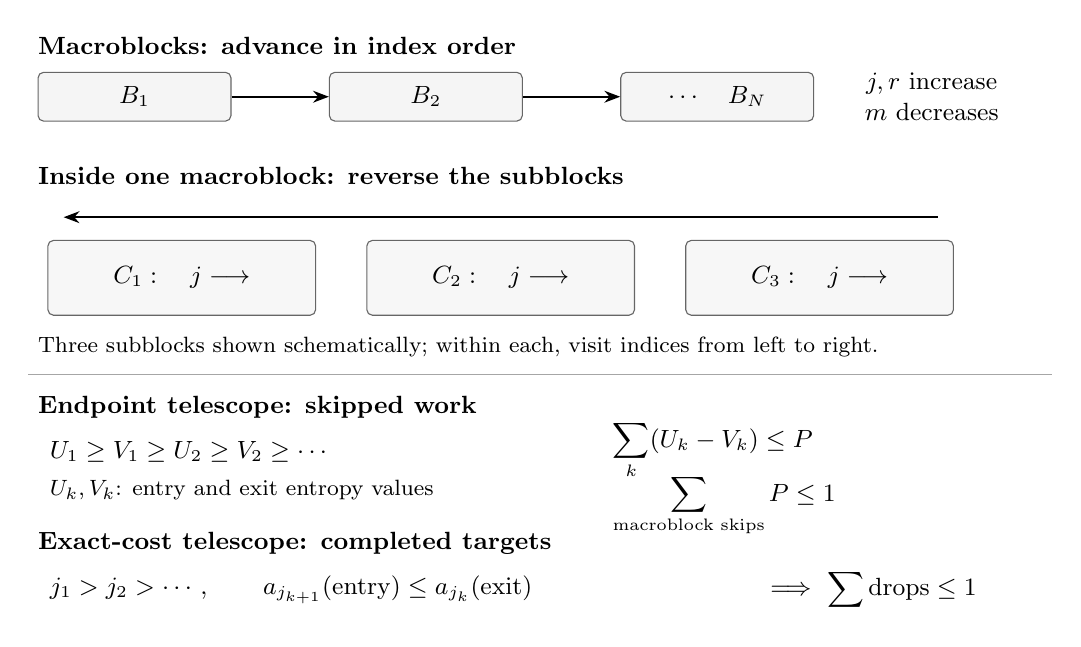
\begin{tikzpicture}[
  x=1cm,y=1cm,font=\small,
  order/.style={-{Stealth[length=2mm]},thick},
  block/.style={draw=black!60,rounded corners=2pt,
    fill=black!4,minimum width=2.45cm,minimum height=.62cm},
  subblock/.style={draw=black!60,rounded corners=2pt,
    fill=black!3,minimum width=3.4cm,minimum height=.95cm},
  note/.style={align=left,anchor=west}
]
 \node[note,font=\small\bfseries] at (0,0)
   {Macroblocks: advance in index order};
 \node[block] (B1) at (1.35,-.65) {$B_1$};
 \node[block] (B2) at (5.05,-.65) {$B_2$};
 \node[block] (B3) at (8.75,-.65) {$\cdots\quad B_N$};
 \draw[order] (B1.east)--(B2.west);
 \draw[order] (B2.east)--(B3.west);
 \node[note,align=center] at (10.5,-.65)
   {$j,r$ increase\\$m$ decreases};

 \node[note,font=\small\bfseries] at (0,-1.65)
   {Inside one macroblock: reverse the subblocks};
 \draw[order] (11.55,-2.18)--(.45,-2.18);
 \node[subblock] (C1) at (1.95,-2.95)
   {$C_1:\quad j\longrightarrow$};
 \node[subblock] (C2) at (6.0,-2.95)
   {$C_2:\quad j\longrightarrow$};
 \node[subblock] (C3) at (10.05,-2.95)
   {$C_3:\quad j\longrightarrow$};
 \node[note,font=\footnotesize] at (0,-3.83)
   {Three subblocks shown schematically; within each, visit indices from left to right.};

 \draw[black!35] (0,-4.18)--(13.0,-4.18);
 \node[note,font=\small\bfseries] at (0,-4.60)
   {Endpoint telescope: skipped work};
 \node[note] at (.15,-5.16)
   {$U_1\ge V_1\ge U_2\ge V_2\ge\cdots$};
 \node[note,font=\footnotesize] at (.15,-5.65)
   {$U_k,V_k$: entry and exit entropy values};
 \node[note] at (7.3,-5.14)
   {$\displaystyle\sum_k(U_k-V_k)\le P$};
 \node[note] at (7.3,-5.85)
   {$\displaystyle\sum_{\text{macroblock skips}}P\le1$};

 \node[note,font=\small\bfseries] at (0,-6.32)
   {Exact-cost telescope: completed targets};
 \node[note] at (.15,-6.91)
   {$j_1>j_2>\cdots,\qquad
     a_{j_{k+1}}(\mathrm{entry})\le a_{j_k}(\mathrm{exit})$};
 \node[note] at (9.3,-6.91)
   {$\displaystyle\Longrightarrow\ \sum\text{drops}\le1$};
\end{tikzpicture}

 \caption{Visit orders in the refinement search. Macroblocks advance with
 $j$, subblocks inside one macroblock are visited in reverse order, and indices
 inside one subblock again advance with $j$. Block lengths $m$ decrease
 with $j$. The endpoint telescope controls skipped work, while the exact-cost
 telescope controls completed targets. In the first sum, $j_k$ runs through
 skipped indices in one subblock, $U_k=g_{m_{j_k,1}}$ at entry to $j_k$, and
 $V_k=g_{m_{j_k,0}}$ at exit from $j_k$. For a macroblock with highest and
 lowest block-length endpoints $H,\ell$, put
 $P=g_H(\text{entry to the macroblock})-g_\ell(\text{current state})$.
 Each $P$ in the macroblock sum is evaluated at that macroblock's own skip. Entry and exit values include
 changes caused by intervening refinements.}
 \label{entropy-refinement:skip-figure}
\end{figure}

\paragraph{One macroblock.}
Let $c_1$ be the cumulative cost in the current macroblock.
At boundaries before or after subblock runs, skip the rest of the macroblock if
\begin{equation}
 P>c_1/\alpha_1+\delta_1.
 \label{entropy-refinement:macro-skip}
\end{equation}
Target indices decrease strictly between completed subblocks. For successive
such indices $j>j'$, monotonicity in index and time gives
\begin{equation}
 a_{j'}(\text{entry to }j')\le a_j(\text{exit from }j).
 \label{entropy-refinement:target-telescope}
\end{equation}
Their actual targeted decreases telescope to at most one. At most $1/u$
subblocks can complete targets, whereas there are $q_*>1/u$ subblocks.
Thus this macroblock must be skipped or discover the desired inequality
before it can be exhausted.

For a completed subblock after which no macroblock skip is made and processing
continues, apply \Cref{entropy-refinement:subblock-cost} with the new $P$,
and then the failure of \Cref{entropy-refinement:macro-skip}:
\[
 c_{1,\mathrm{new}}-c_{1,\mathrm{old}}
 \le\alpha_0(c_{1,\mathrm{new}}/\alpha_1+\delta_1+n^{-2/5}).
\]
Put $\beta_*=\alpha_0/\alpha_1=1/(1000\log N)$ and
$\delta_*=\delta_1+n^{-2/5}$. Iteration over at most $1/u$ such runs yields
\begin{equation}
 c_1\le\alpha_1\delta_*\bigl((1-\beta_*)^{-1/u}-1\bigr)\le\alpha_1.
 \label{entropy-refinement:macro-cost}
\end{equation}
Indeed $n\ge N^5$, so $n^{-2/5}\le N^{-2}$. Also
$-\log(1-\beta_*)\le2\beta_*$, and hence
$(1-\beta_*)^{-1/u}\le N^{1/500}$. The factor multiplying $\alpha_1$ is
at most $N^{-249/500}+N^{-999/500}<1$ for $N\ge4$.
One last or partial subblock costs at most $2\alpha_0$ by
\Cref{entropy-refinement:subblock-cost} and $P\le1$.

\paragraph{Across macroblocks and termination.}
Macroblocks advance in index order, so their block-length ranges descend as in
\Cref{entropy-refinement:mirror-telescope}. The values of $P$ at macroblock
skips sum to at most one. Their total cost is at most $\alpha_1$, and fewer
than $1/\delta_1=\sqrt N$ macroblocks can be skipped.
Since a macroblock cannot be exhausted without a skip or discovery, the
whole search must discover the desired $K$ inequality. Its loops are finite
by the positive minimum offer before clipping. Total cost through discovery
is bounded by
\[
 \underbrace{\alpha_1}_{\text{skipped macroblocks}}
 +\underbrace{\alpha_1}_{\text{continuing subblocks}}
 +\underbrace{2\alpha_0}_{\text{last subblock}}\le4\alpha_1.
\]
Both telescopes allow decreases caused by intervening refinements;
see \Cref{entropy-refinement:skip-figure}.

Since $h=4\log w$ and $M\asymp w^2$, both $\log n$ and $\log N$ are of
order $h$. Thus $4\alpha_1\le C/h^2$. Undoing the cost normalization proves
\Cref{entropy-refinement:search-conclusion}. Each new observation and mark
has a finite alphabet, so the finite sequence leaves a finite-valued context.
\end{proof}

\subsection{Freezing contexts and extracting one phase region}

\begin{proof}[Completion of the proof of \Cref{lemma:compression}]
Use the context $W$, index $j$, and high endpoint $m=m_{j,1}$ supplied by
\Cref{entropy-refinement:search}. Put $r=r_j$ and $s=mr\ge L$.
Combining \Cref{entropy-refinement:search-conclusion} with the low-end bound
\Cref{eq:source-3}, preserved under refinement, gives
\begin{equation}
 K_m(W;r)\le CE
 \label{entropy-refinement:high-cost}
\end{equation}
with numerical $C$. Lift a minimizing coupling to all $s$ letters using
the full-vector interpretation of the cost. Write
$\boldsymbol W=(W_i)_{i=1}^s$ for their whole context stack, and $\nu_z$
for the prescribed one-letter conditional law given context $z$.

At any fixed stack $\boldsymbol w$ of positive probability, compute
\begin{equation}
 \begin{split}
 C(\boldsymbol w)&=
 D\left(X^s\,\middle\|\,\prod_i\nu_{w_i}\right)
 +\mathrm I(X^s;Z)+\E c(\Gamma),\\
 &\hspace{35mm}Z=\sum_iX_i+\Gamma,
 \end{split}
 \label{entropy-refinement:frozen-cost}
\end{equation}
under the actual conditional law at that stack. All three terms are
nonnegative. The actual conditional letter marginals after freezing the
whole stack may differ from the comparator laws $\nu_{w_i}$.
Nevertheless the comparison has finite divergence: an event
$X_i=x,W_i=w_i$ with $\nu_{w_i}(x)=0$ has zero probability even before
conditioning, so it also has zero probability at any positive-probability stack.
Before freezing, however, each row has its prescribed independent block
marginal, and consequently
\[
 \E\left[-\log\prod_i\nu_{W_i}(X_i)\right]=s\mathrm H(X\mid W).
\]
Subtracting $\mathrm H(X^s\mid Z,\boldsymbol W)$ and adding the error cost
therefore shows that $\E C(\boldsymbol W)=K_m(W;r)\le CE$.

For the separate quantity
$B(\boldsymbol w)=s^{-1}\sum_iD(\nu_{w_i}\|U_S)$, the prescribed pair
marginals give
\begin{equation}
 \begin{split}
 \E B(\boldsymbol W)
 &=\log|S|-\mathrm H(X\mid W)\\
 &=\log|S|-\mathrm H(\nu)+G_1(\varnothing)-G_1(W)\\
 &\le CE/T+\frac{CD_*^2}{Eh^2}
 \le\frac{C(D_0)d^2}{Eh^2}.
 \end{split}
 \label{entropy-refinement:frozen-divergence}
\end{equation}
This uses \Cref{eq:source-2,entropy-refinement:search-conclusion}.
The $E/T$ term is absorbed because $T\asymp d/h^5$, $E\le D_0d$, and
$E^2h^7/d^3\to0$ for fixed $D_0$.
Markov's inequality, with factor four for each quantity, selects one stack
such that
\begin{equation}
 C(\boldsymbol w)\le CE,\qquad
 B(\boldsymbol w)\le\frac{C(D_0)d^2}{Eh^2}.
 \label{entropy-refinement:chosen-stack}
\end{equation}
A zero-mean quantity is zero almost surely, which covers that case as well.
Freeze this stack.

\paragraph{A large independent noisy-sum atom.}
Let $p=\prod_i\nu_{w_i}$, and compare the actual conditional law of
$(X^s,\Gamma)$ to the independent law $p\times q$.
The map $(X^s,\Gamma)\mapsto(X^s,Z)$ is invertible, and
$-\log q(\Gamma)=F_0+c(\Gamma)$. Thus
\begin{equation}
 C(\boldsymbol w)=D\bigl((X^s,\Gamma)\|p\times q\bigr)
                   +\mathrm H(Z)-F_0.
 \label{entropy-refinement:noisy-identity}
\end{equation}
Let $Q_Z$ be the sum law under $p\times q$. Data processing gives
\[
 C(\boldsymbol w)+F_0
 \ge D(\mathcal L(Z)\|Q_Z)+\mathrm H(Z)
 =\E[-\log Q_Z(Z)].
\]
Some integer $z_*$ in the support of the actual output therefore has
$Q_Z(z_*)\ge e^{-F_0-CE}=q(0)e^{-CE}$.
All $Q_Z$ masses are positive since $q$ is strictly positive.
Divide the convolution formula by $q(0)$ and use the characteristic formula:
\begin{equation}
 \begin{split}
 e^{-CE}
 &\le Q_Z(z_*)/q(0)\\
 &=\int\chi_{gz_*}(\theta)
       \prod_i\E_{\nu_{w_i}}\chi_{-gX}(\theta)\,d\omega(\theta)\\
 &\le\int\prod_i
       \left|\E_{\nu_{w_i}}\chi_{gX}(\theta)\right|\,d\omega(\theta).
 \end{split}
 \label{entropy-refinement:phase-product}
\end{equation}
The last step takes the absolute value of the preceding integral, whose
value is a positive real mass.

\paragraph{One region and one coordinate.}
Put $\phi_i(\theta)=\E_{\nu_{w_i}}\chi_{gX}(\theta)$ and
$A(\theta)=\sum_i(1-|\phi_i(\theta)|^2)$.
The bound $0\le|\phi_i|\le1$ implies
$\prod_i|\phi_i|\le e^{-A/2}$.
Choose a numerical $C_R$ larger than twice the constant in
\Cref{entropy-refinement:phase-product}, with a fixed additional margin, and
set $\mathcal R=\{A\le C_RE\}$.
Since $E\ge d/h^2\ge1$, the contribution of $\mathcal R^c$ to the product
integral is at most half its lower bound. The product is at most one, so
\begin{equation}
 \omega(\mathcal R)\ge e^{-CE},\qquad
 \sum_i\int(1-|\phi_i|^2)\,d\omega_{\mathcal R}\le CE,
 \label{entropy-refinement:region}
\end{equation}
where $\omega_{\mathcal R}$ is normalized restriction to $\mathcal R$.
Apply Markov's inequality to a uniform choice of coordinate, using
\Cref{entropy-refinement:chosen-stack,entropy-refinement:region}.
One coordinate satisfies both
\begin{equation}
 \int(1-|\phi_i|^2)\,d\omega_{\mathcal R}\le CE/s,\qquad
 D(\nu_{w_i}\|U_S)\le\frac{C(D_0)d^2}{Eh^2}.
 \label{entropy-refinement:coordinate}
\end{equation}
Only numerical factors are lost in the first bound. Write $\mu=\nu_{w_i}$.

\paragraph{A center and a subset valid for every weight.}
For independent $X,\breve X\sim\mu$,
\[
 1-|\phi_i(\theta)|^2
 =\E[1-\operatorname{Re}\chi_{g(X-\breve X)}(\theta)].
\]
Averaging over $\omega_{\mathcal R}$ and then over $\breve X$ selects
$x_0\in\operatorname{supp}\mu\subset S$ with
\[
 \sum_x\mu(x)\int(1-\operatorname{Re}\chi_{g(x-x_0)})
       \,d\omega_{\mathcal R}\le CE/s.
\]
Prune by Markov's inequality to a subset $S'\subset\operatorname{supp}\mu$
of $\mu$-mass at least $1/2$, on which every $x$ satisfies
\begin{equation}
 \int(1-\operatorname{Re}\chi_{g(x-x_0)})\,d\omega_{\mathcal R}\le CE/s.
 \label{entropy-refinement:pruned-defect}
\end{equation}
If the average defect is zero, its zero-defect set has full $\mu$-mass and
can be used for $S'$. In all cases $S'$ is nonempty.

Write $t=\mu(S')\ge1/2$ and $v_0=|S'|/|S|$. Binary data processing gives
\[
 D(\mu\|U_S)\ge
 t\log\frac t{v_0}+(1-t)\log\frac{1-t}{1-v_0}
 \ge t\log\frac1{v_0}-\log2.
\]
Together with \Cref{entropy-refinement:coordinate}, this implies
\[
 \log|S|-\log|S'|\le2D(\mu\|U_S)+2\log2
 \le\frac{C(D_0)d^2}{Eh^2}.
\]
The constant is absorbed because $d^2/(Eh^2)\to\infty$.

Finally, let $v$ be any probability measure on this same $S'$.
By \Cref{entropy-refinement:pruned-defect}, its averaged phase defect on
$\mathcal R$ is at most $CE/s$. Jensen's inequality and $L\le s$ yield
\[
 \begin{split}
 &\int\exp\left[-L\sum_{x\in S'}v(x)
       (1-\operatorname{Re}\chi_{g(x-x_0)}(\theta))\right]\,d\omega(\theta)\\
 &\quad\ge\omega(\mathcal R)
   \exp\left[-L\sum_{x\in S'}v(x)
       \int(1-\operatorname{Re}\chi_{g(x-x_0)})\,d\omega_{\mathcal R}\right]\\
 &\quad\ge e^{-CE}e^{-CEL/s}\ge e^{-CE}.
 \end{split}
\]
The region, center, and subset were fixed before $v$ was chosen, establishing
the conclusion for every probability on $S'$.
The exponential constant is numerical: dependence on $D_0$ occurs in the
entropy loss and in the sufficiently large threshold for $d$, whereas
\Cref{entropy-refinement:high-cost} and all subsequent constant-factor
selections have numerical bounds. This completes the proof.
\end{proof}

\section{Thermal labels and the spectral update}\label{sec:thermal}

This section constructs the channels that will be attached to the spatial
pieces.  It also supplies two ways to pay for a change of channel: a
deterministic increase in a metric ball, and an observable event that is
unlikely under a comparison law.  The choices of channels and of input
membership sets will always be made without inspecting a sampled label.

\subsection{Positive Fourier kernels and form order}

\begin{definition}[Thermal forms]
A thermal form on the unit circle is a finite sum
\[
 A(y)=\sum_s\lambda_s(1-\operatorname{Re}\chi_s(y)),
 \qquad \lambda_s\ge0,\quad s\in\mathbb Z.
\]
We write $A\preceq A'$ if $A'=A+D$ for a thermal form $D$.  Define
\begin{equation}\label{eq:thermal-definitions}
 \begin{gathered}
 q_A(u)=\int_{\mathbb T}e^{-A(y)}\overline{\chi_u(y)}\,dy,
 \qquad F(A)=-\log q_A(0),\qquad K_A=e^{F(A)-A},\\
 \Delta_A(u)=\left(\int_{\mathbb T}|1-\chi_u(y)|^2K_A(y)\,dy\right)^{1/2},
 \qquad B_A(r)=\{u\in\mathbb Z:\Delta_A(u)\le r\}.
 \end{gathered}
\end{equation}
Thus $K_A$ is a probability density.  All circle integrals in this section
use normalized measure of total mass one.
\end{definition}

The covariance argument below belongs to the Griffiths--Ginibre
positive-correlation method \cite{Ginibre1970}. We include the circle
calculation, together with the form-order consequences needed for the
label updates.

\begin{lemma}[Thermal positivity and monotonicity]\label{lemma:thermal-monotonicity}
For every thermal form, $q_A$ is a nonnegative, even probability mass
function on $\mathbb Z$.  The coefficients
$\int\chi_uK_A=q_A(u)/q_A(0)$ are real and nonnegative.  For all integers
$u,v$,
\[
 \operatorname{Cov}_{K_A}(\operatorname{Re}\chi_u,
                          \operatorname{Re}\chi_v)\ge0.
\]
Consequently these characteristic coefficients increase in form order,
$\Delta_A(u)$ decreases in form order, and
$\Delta_A(u+v)\le\Delta_A(u)+\Delta_A(v)$.  The function $F$ increases in
form order.  For every thermal form $D$, the increment
$F(A+D)-F(A)$ decreases when $A$ increases in form order.

If $P=\sum_jP_j$ is a finite sum of thermal forms and
$P_{\rm lo}\preceq P\preceq P_{\rm hi}$, then, for
arbitrary shifts $z_j$ and every integer $u$,
\begin{equation}\label{eq:thermal-envelope}
 \left|\int\chi_u(y)\prod_j e^{-P_j(z_j-y)}\,dy\right|
 \le q_P(u)
 \le e^{-F(P_{\rm lo})}\int\chi_u K_{P_{\rm hi}}.
\end{equation}
\end{lemma}

\begin{proof}
Expand each factor as
\[
 e^{-\lambda(1-\operatorname{Re}\chi_s)}
 =e^{-\lambda}
   \exp\bigl((\lambda/2)\chi_s\bigr)
   \exp\bigl((\lambda/2)\chi_{-s}\bigr).
\]
Its Fourier coefficients are nonnegative, with sum one.  The expansions
are absolutely summable, as is their finite product.  Evaluation at zero
therefore gives $\sum_uq_A(u)=1$; evenness gives $q_A(-u)=q_A(u)$.

For completeness, write $c_s(y)=\cos(2\pi sy)$ and
$Z_A=\int\exp(\sum_s\lambda_sc_s)$.  Express the covariance using two
independent copies as half the expectation of the product of their
differences.  The map $(x,z)\mapsto(x+z,x-z)$ pushes Haar probability on
the two-dimensional torus to Haar probability.  The two differences are
$-2\sin(2\pi ux)\sin(2\pi uz)$ and the analogous expression for $v$,
whereas the unnormalized product density is
$\exp(2\sum_s\lambda_sc_s(x)c_s(z))$.  Expanding this last exponential
gives the identity
\[
 \operatorname{Cov}_{K_A}(c_u,c_v)
 =\frac{2}{Z_A^2}
 \sum_{(n_s)\ge0}\left(\prod_s\frac{(2\lambda_s)^{n_s}}{n_s!}\right)
 \left(\int\sin(2\pi ux)\sin(2\pi vx)
                 \prod_sc_s(x)^{n_s}\,dx\right)^2.
\]
Absolute convergence justifies the expansion and proves nonnegativity.
Differentiation under the integral yields
\[
 \frac{\partial}{\partial\lambda_v}\int c_uK_A
 =\operatorname{Cov}_{K_A}(c_u,c_v),\qquad
 \frac{\partial F}{\partial\lambda_u}=\int(1-c_u)K_A.
\]
The latter derivatives are nonnegative and decrease in every nonnegative
coefficient direction.  Integrating these derivative statements proves
the assertions about $F$ and its increments.  Since
$\Delta_A(u)^2=2(1-\int c_uK_A)$, the metric monotonicity follows as well.
Subadditivity follows from
$1-\chi_{u+v}=(1-\chi_u)+\chi_u(1-\chi_v)$ and the triangle inequality
in $L^2(K_A)$.

Translation multiplies each Fourier coefficient of $e^{-P_j}$ by a
unit complex number.  Absolute values in the convolution of these
coefficients are therefore bounded by the corresponding convolution of
the centered coefficients, which is $q_P(u)$.  Finally
$q_P(u)=e^{-F(P)}\int\chi_uK_P$, and both required comparisons follow
from the monotonicities already proved.
\end{proof}

For a real interval $p$ of length at most one, set
\[
 R_p=|p|^{-1},\qquad
 S_p(y)=R_p^2(1-\operatorname{Re}\chi_1(y)).
\]
The interval may be viewed on the circle when integrating.  We will use
the following bounds, also with any larger spatial scaling in place of
$R_p$:
\begin{equation}\label{eq:thermal-spatial}
 \begin{gathered}
 F(S_p)=\log R_p+O(1),\qquad
 \int(1-\operatorname{Re}\chi_1)K_{A+S_p}\le C R_p^{-2},\\
 q_{S_p}(u)\ge cR_p^{-1}\quad (|u|\le cR_p),\qquad
 \Delta_{A+S_p}(u)\le C|u|/R_p.
 \end{gathered}
\end{equation}
Indeed, if $\|y\|$ denotes distance to the nearest integer, then
$8\|y\|^2\le1-\cos(2\pi y)\le2\pi^2\|y\|^2$.  Gaussian comparison
gives $\int e^{-S_p}\asymp R_p^{-1}$ and
$\int(1-\operatorname{Re}\chi_1)K_{S_p}\le CR_p^{-2}$.  Monotonicity
gives the second bound for $A+S_p$.  The elementary inequality
$|1-\chi_u|\le|u||1-\chi_1|$ gives the last bound and, for sufficiently
small $|u|/R_p$, gives $\int\chi_uK_{S_p}\ge1/2$, proving the remaining
lower bound.  In particular $\int S_pK_{A+S_p}\le C$.

\subsection{Channels, scales, and the cost of tightening a form}

Take $b_0$ dyadic with $h^{-16}/2<b_0\le h^{-16}$.  The computation
levels are the dyadic $b$ from $b_0/8$ to $1$, and
\begin{equation}\label{eq:thermal-parameters}
 k_b=A_0\frac d h(1+\log(1/b))^2,\qquad
 r_{\rm sep}=h^{-30},\qquad \sigma=h^{-40}.
\end{equation}
The constants will be fixed in the order stated below.  Every estimate
holds for sufficiently large $d$, uniformly in the spatial depth and in
any frequency cutoff.

A label of type $A$ is $Z=Y+\theta$ modulo one, where the error $\theta$
has density $K_A$.  Initially $A=0$, so a dummy independent uniform label
may be drawn.  Only the current main channel is used in the spectra and
transforms.  A successful update adds a spatial form and a metric form,
$A^+=A+S_p+D_i$.  The errors used for different label draws are
independent given $Y$.  Their parameters are selected from spatial
prefixes and earlier input membership events.  In particular neither a
sampled old label nor a sampled fresh label selects a membership set,
channel, or test.  Conditional on $Y$ and its discrete parameter path,
the errors thus retain their prescribed independent laws.

We will need to tighten the forms of past labels at small free-energy
cost and to keep their own-error energies $\int A K_A$ small. Both estimates
follow by choosing each metric addition on a sufficiently flat interval of
free energy. We require, with $A_{\rm base}$ the form immediately before
the addition and including its new spatial term,
\begin{equation}\label{eq:source-5}
 F(A_{\rm base}+h^{140}D_i)-F(A_{\rm base}+D_i/2)
 \le d h^{-400}.
\end{equation}
Before a requested update assume that fewer than $C_0h$ main additions
have occurred and that
\begin{equation}\label{eq:source-6}
 F(A)\le\log R_*+C_*d.
\end{equation}
Here $p_*$ is the interval of the most recent addition, $R_*=R_{p_*}$,
and the current $p$ is contained in $p_*$.  Before the first addition
$p_*$ is the top interval, whose length lies in $[1/2,1]$.  The procedure
in \Cref{sec:procedure} will establish these hypotheses inductively.

Fix a sufficiently large numerical $C_s$ and put
$\widetilde A=h^{130}A+C_sS_p$.  Then
\begin{equation}\label{eq:source-7}
 \begin{split}
 F(\widetilde A)-F(A+S_p)
  &\le C+CC_0h\bigl(dh^{-400}+C\log h\bigr),\\
 \int A K_A&\le CC_0h\bigl(dh^{-400}+1\bigr).
 \end{split}
\end{equation}
To prove the first line, enlarge the constituent forms one at a time.
For an old metric term $D_i$, decreasing increments bound its cost of
tightening by the left side of \Cref{eq:source-5}: the other terms already
contain its original $A_{\rm base}$.  Tightening an old spatial term
costs at most
$F(h^{130}S_{p_i})-F(S_{p_i})\le C(1+\log h)$ by
\Cref{eq:thermal-spatial}.  Tightening the current newly inserted $S_p$
to $C_sS_p$ costs $O(1)$.  For the energy bound, concavity along the
$D_i$ direction and \Cref{eq:source-5} give
\[
 \int D_iK_A\le
 2\{F(A_{{\rm base},i}+D_i)-F(A_{{\rm base},i}+D_i/2)\}
 \le2dh^{-400}.
\]
Each spatial constituent contributes $O(1)$ by
\Cref{eq:thermal-spatial} and monotonicity.  This energy argument uses
the count bound and \Cref{eq:source-5}, but does not use
\Cref{eq:source-6}; it remains valid, with the same type of bound, just
after a final allowed addition that breaches a later stopping cap.

The spatial increment itself obeys
\begin{equation}\label{eq:thermal-spatial-increment}
 F(A+S_p)\le F(A)+\log(R_p/R_*)+C.
\end{equation}
After an addition, $A$ contains $S_{p_*}$, so
$q_A(u)\ge ce^{-F(A)}$ for $|u|\le cR_*$.  Convolution with $q_{S_p}$
over those integers gives
$q_{A+S_p}(0)\ge ce^{-F(A)}R_*/R_p$.
Initially use the term $u=0$ alone and $1\le R_*\le2$.

\subsection{From a separated spectrum to a finite compression problem}

Consider a subdensity $a$ at an interval $p$, with
\[
 0\le a\le e^d,\qquad e^{-d}\le m=\mathbb E_pa\le2\alpha,
 \qquad \alpha>0.
\]
Here $\mathbb E_p$ is uniform spatial average, and $\mathcal P$ is the
law of $Y$ with density $a/m$ relative to that average.  For either
prospective child $p'$ define
\begin{equation}\label{eq:thermal-child-moments}
 \begin{split}
 M_{p'}(z)&=\mathbb E_{p'}[aK_A(z-Y)]/\alpha,\\
 f_{p'}^u(z)&=\mathbb E_{p'}[a\chi_u(Y)K_A(z-Y)]/\alpha,\\
 G_{p'}^u&=\int |f_{p'}^u(z)|^2/M_{p'}(z)\,dz.
 \end{split}
\end{equation}
The integrand is zero at zero mass.  An integer is high at $b$ when
some $G_{p'}^u\ge b^2$.  A test requests an update if there is a
collection of $\lceil e^{k_b}\rceil$ high integers whose pairwise
differences avoid
\begin{equation}\label{eq:thermal-separation}
 B_A(r_{\rm sep})+\{j\in\mathbb Z:|j|\le\sigma R_p\}.
\end{equation}
One offending level and one collection are used at a time.

Keep at least half this collection having a common high child, and snap
each retained integer to a nearest multiple $gx$, where
\[
 g=\max(1,\lfloor\sigma R_p/20\rfloor).
\]
The snapping error is at most $\sigma R_p/20$, and is zero when $g=1$.
The snapped indices are distinct, since otherwise the original
difference would violate \Cref{eq:thermal-separation}.  Denote by $S$ the resulting set of integer indices $x$.  For each $x\in S$ choose a measurable complex function
$v_x$, with $|v_x|\le1$, so that
\begin{equation}\label{eq:source-8}
 \operatorname{Re}\mathbb E_{\mathcal P}
  [\mathbf1_{\rm child}v_x(Z)\chi_{gx}(Y)]\ge\beta,
 \qquad \beta=b^2/100.
\end{equation}
The expectation here includes the type-$A$ channel.  To see the bias,
$|f_{p'}^u|\le M_{p'}$ implies $\int|f_{p'}^u|\ge G_{p'}^u$.
Choosing the polarizing sign gives bias
$(\alpha/(2m))\int|f_{p'}^u|\ge b^2/4$ before snapping.  A constant
phase rotation at the center of $p$ makes the error of replacing $u$
by $gx$ at most $C\sigma$.  This is smaller than the required slack
because $\sigma=o(b^2)$ uniformly over the computation levels.

We apply \Cref{lemma:compression} with
\[
 d\omega=K_{\widetilde A}\,dy,\qquad
 q(x)=\frac{q_{\widetilde A}(gx)}{N_g},\qquad
 N_g=\sum_{x\in\mathbb Z}q_{\widetilde A}(gx).
\]
The spatial frequency-one term makes every Fourier coefficient strictly
positive: in its exponential expansion, every integer frequency occurs
with positive coefficient.  Therefore $q$ is strictly positive.  The
grid identity and Gaussian comparison give
\begin{equation}\label{eq:thermal-grid-normalizer}
 N_g=\frac1g\sum_{l=0}^{g-1}e^{-\widetilde A(l/g)},\qquad
 \frac1g\le N_g\le\frac Cg.
\end{equation}
Indeed $g\le R_p$, and the summands are bounded by
$\exp(-cR_p^2\|l/g\|^2)$.  Moreover $R_p/g\le C/\sigma$, also when
$g=1$ by its definition.  Thus \Cref{eq:source-6,eq:source-7,eq:thermal-spatial-increment}
imply
\[
 F_0=-\log q(0)=F(\widetilde A)-\log g+O(1)\le D_0d
\]
for a fixed sufficiently large $D_0$ depending only on the fixed caps.
Evenness gives precisely
$q(x)/q(0)=\int\chi_{gx}\,d\omega$.

We verify both remaining uniform hypotheses of compression.

\paragraph{Sumset size.}
We use the dissociated-spectrum method underlying Chang's lemma
\cite[Section~3]{Chang2002}, in its entropy and positive-product form
\cite[Section~3.2]{Lee2017}. The following calculation includes the side
information carried by the label: the comparison law makes that
information independent of the uniform circle coordinate.

The law of $gY$ modulo one has density at most
$e^{2d}(1+R_p/g)$: its preimage count in $p$ is at most $g/R_p+1$,
and the density of $Y$ relative to circle length is at most $R_pe^{2d}$.
Also
\begin{equation}\label{eq:thermal-label-information}
 \mathrm I(Y;Z)\le F(A)-\log R_*+C.
\end{equation}
Compare each $K_A(z-Y)$ to the fixed density
$K_{S_{p_*}}(z-\operatorname{center}(p_*))$.  The average relative
entropy is
\[
 F(A)-F(S_{p_*})-\int AK_A
 +\mathbb E S_{p_*}(\theta+Y-\operatorname{center}(p_*)).
\]
The last expectation is $O(1)$: use
$S(v+w)\le2S(v)+2S(w)$, the spatial energy bound, and
$|Y-\operatorname{center}(p_*)|\le|p_*|/2$.  In the initial case $A=0$
and $R_*\le2$, the same bound is immediate.  Dropping the nonpositive
term proves \Cref{eq:thermal-label-information}.

Let $Q$ denote the side information consisting of $Z$ and the child
bit.  Data processing and its one-bit entropy imply
\[
 D\bigl((gY,Q)\,\|\,\text{uniform}\otimes\mathcal L(Q)\bigr)
 =D(gY\|\text{uniform})+\mathrm I(gY;Q)\le C(C_*)d.
\]
If $\Lambda\subset S$ is dissociated, meaning that no nonzero
coefficient choice from $\{0,\pm1\}$ sums to zero, form the positive
product
\[
 \prod_{x\in\Lambda}
 \left(1+c\beta\operatorname{Re}
       [\mathbf1_{\rm child}v_x(Z)\chi_x(gY)]\right).
\]
For sufficiently small numerical $c$, the factors lie in $[1/2,3/2]$.
Under the reference law the first coordinate is uniform and independent
of $Q$; expansion and dissociation make the expectation of the product
exactly one.  Relative entropy is at least the true expected logarithm
of this product.  The inequality $\log(1+s)\ge s-Cs^2$, together with
\Cref{eq:source-8}, bounds the expected logarithm of each factor below
by $c'\beta^2$.  Hence $|\Lambda|\le C(C_*)d/\beta^2$.
A maximal dissociated subset spans $S$ by coefficients $0,\pm1$:
otherwise adjoining an unspanned element preserves dissociation.
Consequently
\[
 |nS|\le(2n+1)^{|\Lambda|},\qquad
 \log|nS|\le D_0d h^{P_0}\log d\quad(1\le n\le d^2)
\]
for fixed $D_0,P_0$, because $\beta\ge c h^{-32}$.

\paragraph{The uniform moment cap.}
For any probability $\nu$ on $S$ set
\begin{equation}\label{eq:thermal-moment-cost}
 \begin{split}
 E_T(\nu)&=-\log\mathbb E_\nu
 H_q\left(\sum_{i=1}^TX_i-\sum_{i=1}^TX_i'\right),\\
 e^{-E_T(\nu)}&=
 \int\left|\sum_x\nu(x)\chi_{gx}(y)\right|^{2T}K_{\widetilde A}(y)\,dy,
 \end{split}
\end{equation}
where the $2T$ letters are independent with common law $\nu$.  Then
\begin{equation}\label{eq:thermal-moment-cap}
 0\le E_T(\nu)\le D_0d\qquad\hbox{for every such }\nu.
\end{equation}
Here is a direct proof of the upper bound.  Restrict $Z$ to the domain
$\Omega$ at circle distance at most $h^{40}/R_*$ from $p$.  The channel
spatial variance bounds the discarded probability by $Ch^{-80}$
(the assertion is trivial if $\Omega$ is the full circle).
This loses $o(\beta)$ in \Cref{eq:source-8}.  Summing the biases with
weights $\nu$ and applying Jensen on a subprobability measure gives
\[
 \mathbb E_{\mathcal P}
 \left[\mathbf1_{\rm child}\mathbf1_{\{Z\in\Omega\}}
 \left|\sum_x\nu(x)v_x(Z)\chi_{gx}(Y)\right|^{2T}\right]
 \ge(\beta/2)^{2T}.
\]
For an upper bound discard the child indicator.  At fixed $z$, first
majorize the nonnegative moment integrand using the spatial density
bound $R_pe^{2d}$ and
\[
 \mathbf1_p(y)\le
 \exp\bigl(C-S_p(y-\operatorname{center}(p))\bigr).
\]
Only after this majorization expand the even power and the shifted
thermal weights.  By \Cref{eq:thermal-envelope}, the Fourier
coefficients of those weights are bounded absolutely by
\[
 Cq_{A+S_p}(u)\le
 Ce^{-F(A+S_p)}\int\chi_u K_{\widetilde A}.
\]
The coefficients $v_x(z)$ have modulus at most one.  The absolute
coefficient sum in the even-power expansion therefore averages this
envelope at $u=g(\sum X_i-\sum X_i')$ over the independent letters in
\Cref{eq:thermal-moment-cost}.  Using $|\Omega|\le Ch^{40}/R_*$, the
joint moment is at most
\[
 C R_p e^{2d+F(A)}\frac{h^{40}}{R_*}
       e^{-F(A+S_p)}e^{-E_T(\nu)}.
\]
Now $F(A+S_p)\ge\log R_p-C$,
$F(A)\le\log R_*+C_*d$, and
$T\log(2/\beta)=o(d)$.  Comparison with the lower moment proves
\Cref{eq:thermal-moment-cap} after increasing the fixed $D_0$.
This argument uses a density bound only in a nonnegative integral; it
does not assert a Fourier coefficient bound for $a$.

\subsection{The iterative update and the deterministic alternative}

\begin{lemma}[Spectral update]\label{lemma:spectral-update}
Fix $C_0,C_*\ge1$.  Let the current form $A$ arise from the initial
form zero by fewer than $C_0h$ additions of spatial and metric forms,
each metric satisfying \Cref{eq:source-5}.  Let $p\subset p_*$, where
$p_*$ is the latest addition interval, or the top interval of length in
$[1/2,1]$ if there has been no addition, and assume
$F(A)\le\log R_{p_*}+C_*d$.  On $p$ suppose
$0\le a\le e^d$ and $e^{-d}\le m=\mathbb E_pa\le2\alpha$, with
$\alpha>0$.  Suppose there is a request at a computation level $b$ in
the sense of \Cref{eq:thermal-separation}, using the prospective child
moments in \Cref{eq:thermal-child-moments} and the type-$A$ channel.
There are numerical constants $C_1,C_2$
and a sufficiently small numerical $\varepsilon>0$ with the following
property.  After the caps are fixed, choose fixed sufficiently large
$D_0,P_0$, then $A_0$, and finally take $d$ sufficiently large.
A finite deterministic construction supplies a parameter
\[
 d/h^2\le t\le D_0d,\qquad t\ge\varepsilon k_b,
\]
a thermal metric form $D_i=\lambda B$, and an input-only success set.
On success set $A^+=A+S_p+D_i$.  The new metric satisfies
\Cref{eq:source-5} and
\begin{equation}\label{eq:source-9}
 \begin{gathered}
 A^+=A+S_p+D_i,\qquad \int B K_{A^+}\le C_1t/\lambda,\\
 \lambda\ge dh^{200},\qquad h^{140}\lambda\le L,
 \end{gathered}
\end{equation}
and $F(A^+)-F(A+S_p)\le C_1t$.
There are two alternatives:
\begin{enumerate}[label=\textup{(\roman*)}]
 \item A regular test has success probability $\delta\ge\beta/2$ under
 the current input law, where $\beta=b^2/100$.  It also supplies a
 probability $\nu$ on a set $S'$ and a center $x_0\in S$ for which
 $E_T(\nu)\ge t/4$.
 \item A cheap update succeeds deterministically, has
 $t=\varepsilon k_b$, and uses the uniform probability on $S'$.
\end{enumerate}
In both alternatives $\log|S'|\ge0.8k_b$ and
$B=\sum_x\nu(x)(1-\operatorname{Re}\chi_{g(x-x_0)})$.
Track a radius starting at $r_{\rm sep}/4$ and increasing by
$\eta=r_{\rm sep}/(10C_0h)$ at every main addition.  As long as the
count cap applies, the gap $F(A)-\log|B_A(r)|$ starts at zero, stays
bounded below by a numerical negative constant, increases by at most
$C_2t$ at a regular success, and decreases by at least $k_b/2$ at a
cheap success.  On failure there is no main addition and no label draw.
All these conclusions are independent of spatial depth and frequency
cutoff.
\end{lemma}

\begin{proof}
\textbf{Selecting the subset and its weight.}
On $S$ and then on its successive restrictions set
\[
 t=\max\left(\varepsilon k_b,
                 \max_{\nu\text{ supported on the current set}}E_T(\nu)
       \right).
\]
The maximum exists: the simplex is compact, its moment integral is
continuous and strictly positive, and therefore its negative logarithm
is continuous.  For large $d$, the floor is between $d/h^2$ and $D_0d$;
the upper bound follows also for the maximum from
\Cref{eq:thermal-moment-cap}.  Apply \Cref{lemma:compression} with
$E=t$ to obtain a subset $S'$ and center $x_0$. Its conclusion holds
for every probability on this fixed $S'$, so the weight may now be chosen
by the following test.
If the maximum of $E_T$ on $S'$ is at least $t/4$, keep a maximizing
witness and terminate with a regular test.  If that maximum is smaller
than $t/4$ and $t=\varepsilon k_b$, take uniform $\nu$ on $S'$ and
terminate with a cheap update.  Otherwise replace the current set by
$S'$ and repeat.  Every nonterminal iteration reduces $t$ by a factor
of at least four, except possibly for the last transition to the fixed
floor.  Thus the process terminates in finitely many iterations, and
the sum of the logarithmic cardinality losses is at most
\[
 C(D_0)\frac{d^2}{\varepsilon k_bh^2}.
\]
The initial child restriction lost at most $\log2$ in logarithmic
cardinality.  Since $k_b\ge A_0d/h$, choosing $A_0$ sufficiently large
in terms of $D_0,P_0,\varepsilon$ makes the final loss less than
$0.2k_b$, proving $\log|S'|\ge0.8k_b$.

\textbf{Choosing a flat coefficient range.}
For the last center and chosen probability, the compression conclusion
is
\[
 F(\widetilde A+LB)-F(\widetilde A)\le Ct.
\]
Put $A_{\rm base}=A+S_p$. Monotonicity of $F$ and
$A_{\rm base}\preceq\widetilde A$ give
\[
 F(A_{\rm base}+LB)-F(A_{\rm base})
 \le \bigl[F(\widetilde A+LB)-F(\widetilde A)\bigr]
       +\bigl[F(\widetilde A)-F(A_{\rm base})\bigr].
\]
The first bracket is controlled by compression and the second by the
tightening bound in \Cref{eq:source-7}. Hence
\begin{equation}\label{eq:thermal-volume-cost}
 F(A_{\rm base}+LB)-F(A_{\rm base})\le C_1t.
\end{equation}
The constant $C_1$ is numerical: the volume constant of compression is
numerical, and the cap-dependent error in \Cref{eq:source-7} is $o(t)$
after the fixed caps and $A_0$ have been selected.

To find a flat range, set
\[
 \lambda_j=dh^{200}(2h^{140})^j,
 \qquad
 N=\left\lfloor
 \frac{\log(2L/(dh^{200}))}{\log(2h^{140})}\right\rfloor.
\]
For $0\le j<N$, the intervals
$[\lambda_j/2,h^{140}\lambda_j]$ are adjacent and lie in
$[dh^{200}/2,L]$.  Since $\log(L/d)=w=e^{h/4}$,
$N\asymp e^{h/4}/\log h>C_1D_0h^{400}$ for sufficiently large $d$.
The sum of the free-energy increments on these intervals is bounded
by \Cref{eq:thermal-volume-cost}, hence by $C_1D_0d$.  At least one
increment is at most $dh^{-400}$.  Take its $\lambda$ and
$D_i=\lambda B$; this is \Cref{eq:source-5}.  Concavity along the
$B$ direction gives
\[
 \int BK_{A_{\rm base}+\lambda B}
 \le\frac{F(A_{\rm base}+\lambda B)-F(A_{\rm base})}{\lambda}
 \le C_1t/\lambda,
\]
which proves \Cref{eq:source-9} and the metric increment bound.

\textbf{The input-only success set.}
For a regular test define the success set by
\begin{equation}\label{eq:thermal-success-set}
 \left|\sum_x\nu(x)\chi_{gx}(Y)
                  \mathbb E[v_x(Z)\mid Y]\right|\ge\beta/2.
\end{equation}
The expectation uses the specified type-$A$ channel, rather than the
sampled old observation.  The expression has modulus at most one, and
\Cref{eq:source-8}, averaged with $\nu$, gives its expected modulus at
least $\beta$.  Thus its probability of exceeding $\beta/2$ is at
least $\beta/2$.  In the cheap alternative take the entire input as
success.  The data $a,p,\alpha,A$ determine all these sets and choices.

\textbf{The change in the gap potential.}
It remains to prove the gap assertions. Since $r\le r_{\rm sep}/2$
through the count cap, summability of $q_A$ gives
\[
 |B_A(r)|e^{-F(A)}(1-r^2/2)\le1,
 \qquad F(A)-\log|B_A(r)|\ge\log(1-r^2/2)\ge-C.
\]
The balls are finite by the same inequality.  Initially $A=0$ and
$B_0(r)=\{0\}$, so the gap is zero.
The spatial addition raises $F$, but also allows short integer translates
of the old ball inside a slightly larger new ball. We compare these changes
using the same overlap multiplicity. Write
\[
 U=B_A(r),\qquad
 D_p=\mathbb Z\cap[-\sigma R_p/10,\sigma R_p/10],\qquad
 l=|(U-U)\cap(D_p-D_p)|.
\]
Here $l\ge1$.  On this intersection $\Delta_A\le2r$ and
$|u|\le\sigma R_p/5$, so convolution and
\Cref{eq:thermal-spatial} imply
\begin{equation}\label{eq:thermal-packing-pair}
 F(A+S_p)-F(A)\le\log R_p-\log l+C,
 \qquad |U+D_p|\ge |U||D_p|/l.
\end{equation}
For the second inequality, each representation of a fixed element of
$U+D_p$ differs from one fixed representation by an element of the
intersection defining $l$, so its multiplicity is at most $l$.

After either addition, $U+D_p$ lies in $B_{A^+}(r+\eta/2)$, since
monotonicity preserves the old radius and
$\Delta_{A^+}(j)\le C|j|/R_p\le C\sigma=o(\eta)$ for $j\in D_p$.
On a cheap success, uniformity of $\nu$ and \Cref{eq:source-9} give
\[
 \frac1{|S'|}\sum_{x\in S'}\Delta_{A^+}(g(x-x_0))^2
 \le 2C_1t/\lambda.
\]
At least half the $x$ therefore have
$\Delta_{A^+}(g(x-x_0))\le\sqrt{4C_1t/\lambda}
\le C(D_0)h^{-100}=o(\eta)$.  Their translates
$g(x-x_0)+U+D_p$ lie in the new tracked ball $B_{A^+}(r+\eta)$.
They are disjoint.  A collision would put $g(x-x')$ in
$U-U+D_p-D_p$; after restoring the two snapping errors, the difference
of the original frequencies would lie in
\[
 B_A(2r)+\{j\in\mathbb Z:|j|\le3\sigma R_p/10\},
\]
contrary to \Cref{eq:thermal-separation}.

Since $R_p/|D_p|\le C/\sigma$, including the case $D_p=\{0\}$,
\Cref{eq:thermal-packing-pair} cancels the same $\log l$ in the
free-energy and cardinality costs.  On a regular success the gap
increase is at most $C_1t+O(\log h)\le C_2t$ for a numerical $C_2$.
On a cheap success it is at most
\[
 C_1\varepsilon k_b-\log(|S'|/2)+O(\log h)
 \le C_1\varepsilon k_b-0.8k_b+O(\log h)\le-k_b/2,
\]
on choosing $\varepsilon$ sufficiently small numerically and then
taking $d$ sufficiently large.  These choices precede the cap choices;
only the size-loss bound and the small-error thresholds require the
subsequent choices of $A_0$ and $d$.
\end{proof}

\subsection{Evidence under the comparison law and under truth}

At every success draw a new main label $V$ of type $A^+$.  On a regular
success also draw $N_h=\lceil h^{120}\rceil$ fresh, independent
type-$A$ clones $Z'$.  They serve only the evidence calculation.
These draws are made even when this very success will breach a cap and
transfer the piece out of live processing.  A failure causes neither a
new main draw nor an evidence draw.

The comparison experiment starts with $Y$ uniform on the top interval.
Spatial bits continue to observe $Y$, and all label draws use the same
channels prescribed on their recorded branches.  At a membership test,
however, success is an independent coin with probabilities
$\delta,1-\delta$ computed from the current true input law before
conditioning on sampled labels.  For a fixed recorded spatial and
membership branch, the computed state is fixed.  Its membership coin
probabilities therefore contribute no $y$-dependent likelihood.  Given
the full past observations at a test in $p$, the comparison posterior
has density on $p$ proportional to
\begin{equation}\label{eq:thermal-reference-posterior}
 \exp\left(-\sum_jA_j(z_j-y)\right).
\end{equation}
The sum includes past main labels and past evidence clones.  Each
$A_j\preceq A$, and their number is at most
$1+C_0h(1+N_h)$.  This statement conditions on the observed branch,
not on the actual truth-membership event within the reference law.

Set $s_d=dh^{-100}$.  A past is admissible when some
$y_0\in\overline p$ satisfies
\[
 \sum_jA_j(z_j-y_0)\le s_d.
\]
This is an observable condition: the continuous function in the display
attains its infimum on the compact interval closure.

\begin{proposition}[Regular evidence]\label{prop:thermal-evidence}
Consider any finite procedure starting with the type-zero label, making
at most $\lfloor C_0h\rfloor$ successful main additions and using the
updates of \Cref{lemma:spectral-update} with its hypotheses at every
attempt.  Require all discrete choices to depend only on spatial
prefixes and input memberships, with independent label errors given
$Y$ and its parameter path, and include all the success draws specified
above.  Then an admissible regular attempt
has the following conditional reference bound, given its past and its
success coin.  The observable event
\begin{equation}\label{eq:source-10}
 \begin{gathered}
 \text{for some fresh clone }Z',\qquad A(Z'-Z)\le4s_d,\\
 \left|\sum_x\nu(x)v_x(Z')\chi_{gx}(V)\right|\ge\beta/4.
 \end{gathered}
\end{equation}
has probability at most $e^{-t/8}$, where $Z$ is the old main label.
Under the true input law, all attempted pasts are admissible and
\Cref{eq:source-10} occurs at every regular success simultaneously,
except on a set of probability $o(h^{-20})$.  This includes the label
draws at a final success breaching a cap.  The bounds are uniform in
depth, cutoff, and the deterministic choices made at the states.
\end{proposition}

\begin{proof}
First bound the posterior normalizing integral from below at an
admissible past.  The phase triangle inequality gives
$A_j(v+u)\le2A_j(v)+2A_j(u)$, and the observation count gives
$2\sum_jA_j\preceq h^{130}A$ for sufficiently large $d$.
Thus
\begin{equation}\label{eq:thermal-posterior-denominator}
 \int_p\exp\left(-\sum_jA_j(z_j-y)\right)dy
 \ge c\exp(-2s_d-F(\widetilde A)).
\end{equation}
Indeed in one direction from $y_0$ a segment of length $|p|/2$ remains
inside $\overline p$.  By symmetry and the spatial variance estimate,
the density $K_{\widetilde A}(y-y_0)$ assigns this segment at least a
numerical positive mass if $C_s$ is large enough: the circular
second-moment bound puts a fixed positive mass within distance $|p|/2$
of zero, and symmetry gives half of that mass in either direction.
On this segment the
integrand is at least
$e^{-2s_d}\exp(-h^{130}A(y-y_0))$, which is at least
$e^{-2s_d}\exp(-\widetilde A(y-y_0))$.

Fix one fresh clone and integrate over its value $z'$ in the
consistency set $\{z':A(z'-Z)\le4s_d\}$.  Also use the variable
$\theta^+=V-Y$, whose independent conditional density is $K_{A^+}$.
At fixed $z',\theta^+$ expand the $2T$-moment of
\[
 \left|\sum_x\nu(x)v_x(z')\chi_{gx}(Y+\theta^+)\right|
\]
in the posterior integral.  Its weights include the extra clone
factor $e^{-A(z'-y)}$ and the spatial majorant used above.  The centered
summed form is
\[
 P=\sum_jA_j+A+S_p,
 \qquad A+S_p\preceq P\preceq\widetilde A.
\]
The upper comparison follows from the observation count and large $d$.
By \Cref{eq:thermal-envelope}, the $y$ integral before the clone
normalization and the posterior division is at most
\[
 Ce^{-F(A+S_p)}e^{-E_T(\nu)}
 \le Ce^{-F(A+S_p)}e^{-t/4}.
\]
Here the phase factors involving $\theta^+$ have modulus one, and
$|v_x(z')|\le1$, so the same coefficientwise moment bound applies.
The consistency set has length at most $e^{4s_d-F(A)}$, since
$e^{-A}\ge e^{-4s_d}$ there.  This cancels the clone normalization
$e^{F(A)}$ up to $e^{4s_d}$.  The density in $\theta^+$ integrates
to one.  Dividing by \Cref{eq:thermal-posterior-denominator}, applying
the moment tail bound at $\beta/4$, and summing over the clones gives
\[
 C N_h\exp\left(
 6s_d+F(\widetilde A)-F(A+S_p)
       +2T\log(4/\beta)-t/4\right)\le e^{-t/8}.
\]
Indeed \Cref{eq:source-7}, $t\ge\varepsilon k_b$, and
$2T\log(4/\beta)=o(t)$ absorb every positive term.  The reference
success coin is independent of $Y$ given the past and so has not
altered its posterior.

For the true-law assertion, condition on $Y$ and its entire discrete
parameter path.  At a regular success the conditional mean in
\Cref{eq:thermal-success-set} has modulus at least $\beta/2$.  The
empirical mean of the $N_h$ clone polynomials evaluated at $Y$
approximates it to error $\beta/16$ except with probability
$C/(\beta^2N_h)$, by the second-moment bound for independent bounded
complex variables.  Replacing $Y$ by $V$, and removing the common
phase $\chi_{gx_0}(V-Y)$, changes each of these polynomials by at most
\[
 \sum_x\nu(x)|1-\chi_{g(x-x_0)}(V-Y)|.
\]
Its conditional expectation is at most
$\sqrt{2\int BK_{A^+}}\le C\sqrt{t/\lambda}=O(h^{-100})$
by \Cref{eq:source-9}.  Markov's inequality makes this error at most
$\beta/16$ except with probability
$C\sqrt{t/\lambda}/\beta=o(h^{-30})$, since
$\beta\ge ch^{-32}$.  Outside these errors the clone average after
replacement has modulus at least $3\beta/8$, so at least one clone
satisfies the large-polynomial condition in \Cref{eq:source-10}.
The empirical-mean error probability is $O(h^{-56})$, also
$o(h^{-30})$.

Finally sum the own-error energies of every observation on the capped
true path, each measured in its own form.  Conditional independence
and the input-only selection rule let us apply the energy estimate in
\Cref{eq:source-7} at each draw, including final draws.  There are at
most $O(h^{121})$ observations, each of conditional expected energy
$O(h(dh^{-400}+1))$.  Their total expected energy is therefore
\[
 O(dh^{-278}+h^{122})=o(s_dh^{-30}).
\]
With exception probability $o(h^{-30})$, their total energy is at
most $s_d$.  This single event makes every past admissible by taking
$y_0=Y$.  It also gives every consistency condition, since the old
main and its clone both have type $A$ and
\[
 A(Z'-Z)\le2A(Z'-Y)+2A(Z-Y)\le4s_d.
\]
There are only $O(h)$ regular successes.  Unioning their conditional
large-polynomial failure bounds and adding the total-energy exception
proves the simultaneous $o(h^{-20})$ assertion.  The bound is over
successes rather than over all attempts; past admissibility at all
attempts followed from the single total-energy event.
\end{proof}

The numerical constants $C_1,C_2$ and the permitted small
$\varepsilon$ have now been fixed independently of the later caps.
The next section chooses those caps, then fixes $D_0,P_0,A_0$, and
finally increases the threshold for $d$. The evidence clones enter only
the likelihood estimate for regular charges. The main labels also enter
the conditional-information bounds for the spatial budgets. The realized
values of both kinds of labels do not control the spatial splitting procedure.

\section{The finite dyadic procedure and its budgets}
\label{sec:procedure}

We seek a bound for modulated sums whose coefficients are formed from one
input bit and emitted with a later output bit. The bound must be uniform
in the tree depth and in the number of frequencies. We state it first;
the construction in this section supplies the pieces and budgets used in
its proof in \Cref{sec:assembly}.

\begin{proposition}[Modulated delayed Haar estimate]\label{prop:dyadic}
There are absolute constants $C$ and $d_0$ with the following property.
Let $d\ge d_0$, put $h=\log\log d$, and let $I\subset\R$ be a half-open
interval with $1/2\le |I|\le1$.  Let $\rho:I\to[0,\infty)$ be measurable,
with $\rho\le e^d$ almost everywhere and
\[
 m_{\rm top}=\frac1{|I|}\int_I\rho\le2.
\]
Give $I$ its normalized uniform probability $\mathbf U$.  Write
$\mathcal F_j$ for its depth-$j$ dyadic sigma field, $p_j(x)$ for the
depth-$j$ interval containing $x$, and $r_{j+1}$ for the sign that is $+1$
on the left child and $-1$ on the right child of each such interval.
Let $J\ge1$ and $Q\ge0$ be integers.  For $0\le j<J$, let
$\epsilon_j:I\to\C$ be $\mathcal F_{j+1}$-measurable with
$|\epsilon_j|\le1$, and use the same $\epsilon_j$ for all modulations.
The bits through depth $J+1$ are retained, so the last output sign is
$r_{J+1}$.

Set
\[
 \tau(x)=\min\bigl(\{0\le j<J:\ \E_{p_j(x)}\rho>e^{4h}\}\cup\{J\}\bigr),
 \qquad \E_p v=\frac1{|p|}\int_p v(y)\,dy,
\]
and, with $\chi_u(y)=e^{2\pi iuy}$, define
\[
 \mathcal H_{I,J}^{u}\rho(x)
 =\sum_{0\le j<\tau(x)}
       \E_{p_j(x)}[\rho(Y)\chi_u(Y)r_{j+1}(Y)]\,
       \epsilon_j(x)r_{j+2}(x).
\]
Then
\begin{equation}\label{eq:dyadic-estimate}
 \int_I\max_{\substack{u\in\Z\\|u|\le Q}}
           |\mathcal H_{I,J}^{u}\rho(x)|\,\frac{dx}{|I|}
 \le Cd.
\end{equation}
The constants are independent of $I,\rho,J,Q$, and the multipliers.
Consequently the same estimate holds with $\sup_{u\in\Z}$ in place of
the finite maximum.
\end{proposition}

\subsection{Input pieces and the order of processing}

Fix the data of \Cref{prop:dyadic}. At an output point $x$ in a depth-$j$
interval $p$, the summand in that proposition is
\begin{equation}
 \mathbb E_p[\rho(Y)\chi_u(Y)r_{j+1}(Y)]\,
       \epsilon_j(x)r_{j+2}(x),\qquad u\in\mathbb Z.
 \label{eq:source-11}
\end{equation}
The input variable $Y$ and output point $x$ play different roles. The
coefficient is known before the output bit $r_{j+1}(x)$, whereas its
multiplier $\epsilon_j(x)$ need only be known before $r_{j+2}(x)$.
The bits retained through depth $J+1$ supply this delayed sign even for
the last contributing jump. The same multipliers are used for every piece
and every label coordinate.

Every piece and frequency uses the common stopping rule $\tau$ of
\Cref{prop:dyadic}, defined from the original density $\rho$. No processing
is needed at a node where this rule has already stopped the output path.
At all other nodes, the processing below is completed before the jump.

Discard the zero input.  If $0<m_{\rm top}<1/h$, put the whole input
into static handling at the top.  Otherwise define the true input law
\[
 d\mathbf P(Y)=\frac{\rho(Y)}{m_{\rm top}}\,d\mathbf U(Y).
\]
The word ``true'' will always refer to this input law, or to its
conditional laws, and not to uniform output sampling.

A processing state at a spatial interval $p$ consists of a subdensity
$a$, its mean $m=\mathbb E_p a$, and its recorded spatial and membership
history.  The subdensity is the restriction of $\rho$ by the membership
sets on that history.  A zero-mass state is discarded.  A live state
also carries a main thermal form $A$, a count $n$ of successful main
additions, and the charge
\[
 \mathcal Q=\sum_{\text{regular successes so far}}t.
\]
Initially $A=0$, $n=0$, and $\mathcal Q=0$.  These three quantities
carry along the entire branch and are never reset at a new epoch or
plateau.

Fix constants $R_0,C_0,C_*$ in the order specified below.  The
processing rules are as follows.
\begin{enumerate}[label=\arabic*.,leftmargin=*]
\item At every incoming live state, transfer its entire current
subdensity to static handling if
\[
 m<e^{-d},\qquad \mathcal Q>R_0d,
       \qquad\text{or}\qquad n\ge\lfloor C_0h\rfloor.
\]
This transfer ends its live processing.  Its density is subsequently
only restricted to spatial descendants; it is never split by another
membership test.

\item The initial live piece starts an epoch.  Every successful main
addition starts a new epoch on its success piece unless that piece
transfers immediately.  Within an epoch, a plateau starts with
normalization $\alpha=m$ at entry.  At a subsequent incoming state it
ends and a new plateau starts if $m>2\alpha$.  The new normalization
is the incoming mean.  No new main label is drawn at such a reset.

\item At a live state that has passed the transfer and reset rules,
apply the spectral test of \Cref{lemma:spectral-update} to
$(a,p,\alpha,A)$, using the prospective child moments.  Thus
$e^{-d}\le m\le2\alpha$.  The tests range over all computation
levels $b\in[b_0/8,1]$ that are powers of two; stabilization means
that at each such level there is no separated high collection of
size $\lceil e^{k_b}\rceil$.  If a test requests an update, its success
set $E$ is a measurable set of inputs, determined from this state.
Replace the current density by the two subdensities
\[
 a\mathbf1_E\quad\hbox{and}\quad a\mathbf1_{E^c}.
\]
Only the success piece receives the new form $A^+$ and the increment
of the count; a regular success also adds $t$ to $\mathcal Q$.
Its mean is $\delta m$, where $\delta$ is its conditional success
probability.  The failure piece, if it has positive mass, has mean
$(1-\delta)m$ and retains the old epoch, plateau, form, and charge.
For a cheap update $\delta=1$.

\item Process both resulting pieces at the same spatial interval
$p$, enforcing transfer and reset rules anew.  Continue until every
remaining live piece at $p$ passes all spectral tests.  Then, and only
then, take the spatial jump for each surviving live piece and each
static piece, and proceed to its children subject to the common stop.
\end{enumerate}

Static pieces also have plateaus: start with normalization equal to
their mean at transfer (or at initial static entry), and restart
whenever the incoming mean exceeds twice that normalization.  They
undergo no spectral tests or membership splits.  Their estimates will
use only the scalar construction.

Every test, witness, and membership set is chosen from the spatial
prefix and the preceding membership outcomes.  In particular, none of
these choices uses a realized noisy observation or the next spatial
bit.  The label experiments are attached to these already specified
discrete branches.  Start with a type-$0$ main observation, independent
of the input.  Draw a fresh main observation of type $A^+$ on every
success.  On a regular success also draw the old-type evidence clones
specified in \Cref{prop:thermal-evidence}.  Make these draws even when
that success immediately causes a transfer.  Moving to a smaller
interval, following a failure, or resetting $\alpha$ does not redraw
the main observation.  Given the input and its discrete branch, every
draw uses fresh independent error with its specified channel law.

At a jumping node the density belonging to a plateau is its final
\emph{post-processing survivor}.  Its prospective child densities
are the restrictions of that survivor, before any processing at the
children.  Removed mass has instead been assigned to another plateau
or to static handling.  Therefore the densities of all jumping pieces
at $p$ sum exactly to $\rho|_p$, and their normalized contributions, after
multiplication by their respective normalizations, sum exactly to
\Cref{eq:source-11}.  A true input follows just one of these pieces;
uniform output estimates must sum all of their starting weights.

\subsection{Statement of the budgets}

For a live plateau $e$, write $p_e$ for its root and $\alpha_e$ for its
initial mean, and put $\mathbf U_e=\mathbf U(\,\cdot\mid p_e)$.
At a final live jumping state $p$ belonging to $e$, use its post
density $a$ and its fixed main channel to define
\[
 M_\pm(z)=\frac{\mathbb E_{p_\pm}[a(Y)K_A(z-Y)]}{\alpha_e},\qquad
 M=\frac{M_++M_-}{2},\qquad
 D=\frac{M_+-M_-}{2},\qquad
 J_p=\int\frac{|D|^2}{M}\,dz.
\]
The piece and plateau are implicit in $J_p$; zero divided by zero is
taken to be zero.  Notice that $\int M=m_p/\alpha_e\le2$, where
$m_p=\mathbb E_p a$, whereas $\int M_\pm\le4$.  In particular
$J_p\le2$.

\begin{proposition}[Live budgets]\label{prop:live-budgets}
There are fixed absolute choices of the constants in the procedure
and in \Cref{lemma:spectral-update} such that, for all sufficiently
large $d$, the procedure is finite in every finite spatial tree and
preserves the exact splitting identity above.  When
$1/h\le m_{\rm top}\le2$, it has the following bounds, with constants
independent of $J$, $I$, the input, and any frequency cutoff.
\begin{enumerate}[label=\textup{(\roman*)},leftmargin=*]
\item Before every requested live update the count and form
hypotheses of \Cref{lemma:spectral-update} hold.  On every input
branch, including its final success if a cap is crossed,
\[
 \sum_{\rm successes}k_b+\sum_{\rm successes}t
       +\sum_{\rm successes}\bigl(F(A^+)-F(A+S_p)\bigr)\le Cd,
 \qquad n\le C h.
\]
The count flag cannot cause transfer unless the charge flag has
already been crossed at that success.

\item Let $B_{\rm mem}$ be the sum of the negative logarithms of the
conditional probabilities of all observed membership outcomes along
the true path through live termination.  Let
$X_* =\max\log^-m$ over its processing states, including the state
at transfer or at the common stop, but excluding later static
descendants.  Then
\begin{equation}
 \|B_{\rm mem}\|_{L^2(\mathbf P)}
       +\|X_*\|_{L^2(\mathbf P)}\le C h,
 \label{eq:source-12}
\end{equation}
and $\mathbf P(\mathrm{transfer})\le C h^{-10}$.

\item The live plateau weights satisfy
\[
 \sum_{e\text{ live}}\mathbf U(p_e)\alpha_e\le C h.
\]
If $\xi_p$ is the local average of mass removed from the survivor of
one plateau at $p$, divided by its $\alpha_e$, then
$\mathbb E_{\mathbf U_e}\sum_p\xi_p\le1$.  Full removal at an exit
may be included.  Starting from a final jumping post state $p_0$,
the corresponding future bound under uniform probability on $p_0$
is at most $m_{p_0}/\alpha_e\le2$.

\item The global label Fisher sum obeys
\begin{equation}
 \sum_{\text{all live jumping pieces }p}
        \mathbf U(p)\alpha_e J_p\le C d.
 \label{eq:source-13}
\end{equation}
\item Ignore the labels and use the filtration of spatial bits and
memberships.  After live termination one may keep the final piece
fixed and reveal any finite number of additional spatial bits, making
no further membership observations.  The expected sum of the spatial
bit relative entropies to a fair bit is $O(d)$.  If this spatial
extension is stopped at the common density cutoff, the bound is
$O(h)$.
\end{enumerate}
\end{proposition}

\begin{proof}
\subsubsection*{Caps, constant order, and finite termination}
Let $C_1$ be the numerical constant bounding a relative metric cost
by $C_1t$ in \Cref{lemma:spectral-update}, and let $C_2$ be its
numerical regular gap-increase constant.  Choose the numerical
$\varepsilon>0$ there small enough for the cheap gap decrease, and
take $R_0=1000$.  Consider a prefix of successes for which the update
hypotheses have been justified.  The gap potential
\[
 F(A)-\log|B_A(r)|
\]
starts at zero and is bounded below by an absolute constant.  Here
$r$ begins at $r_{\rm sep}/4$ and increases by
$r_{\rm sep}/(10C_0h)$ at each addition, so $r\le r_{\rm sep}/2$
under the count cap.  Telescoping its regular increases and cheap
decreases gives
\begin{equation}
 \sum_{\rm cheap}k_b\le
          2C_2\sum_{\rm regular}t+C,
 \qquad
 \sum_{\rm successes}t\le
       (1+2\varepsilon C_2)\sum_{\rm regular}t+C.
 \label{eq:06-gap-accounting}
\end{equation}
In the second inequality we used $t=\varepsilon k_b$ on cheap
successes.  Regular successes also satisfy $\varepsilon k_b\le t$.
Consequently, while $\mathcal Q\le R_0d$, the sum of all success
$k_b$'s is at most $C(R_0,\varepsilon,C_2)d$.  Since every
$k_b\ge d/h$, the number of those successes is at most $C'h$.
Choose $C_0>C'+2$.  A first count breach without a charge breach
would obey this same prefix bound, contradicting that choice for
large $d$.

The form cap is also inductive.  If the preceding main addition
occurred at $p_*$, the spatial and metric estimates give
\[
 F(A^+)-F(A)
       \le\log(R_p/R_*)+C+C_1t.
\]
The spatial scale ratios telescope along a branch.  Before a charge
breach, \Cref{eq:06-gap-accounting} and the count estimate therefore
give $F(A)\le\log R_*+C_*d$ for a sufficiently large fixed $C_*$.
The initial case is $A=0$ with $p_*=I$.  At the next update, the
flat-increment condition \Cref{eq:source-5} is supplied by the update
itself.  Thus the assumptions needed to construct each successive
update have been established from its predecessors.

Fix $D_0,P_0$ in the compression application using these caps, then
fix $A_0$ sufficiently large for the cardinality loss, and finally
take $d$ sufficiently large for all required asymptotic inequalities.
The constants $C_1,C_2$ and the choice of $\varepsilon$ precede the
caps; their numerical nature is what permits this order.  A regular
success that first crosses the charge cap adds at most $D_0d$ and
is followed immediately by transfer.  Hence that final overshoot
only changes the absolute constants in the claimed path budgets.
No subsequent update uses a form cap for this terminal form.  The
energy estimate in \Cref{eq:source-7} remains valid for the labels
drawn at that success, as it uses the flat-increment and count bounds.
This proves all the deterministic budget assertions.

At a fixed spatial node, the number of successes along any recurrence
path is bounded by the count cap.  Between successes, every failure
multiplies $m$ by at most $1-c(b_0/8)^2$.  Since $m\le e^d$, only
finitely many consecutive failures are possible before $m<e^{-d}$.
There is a uniform finite bound, depending on $d$ but not the node,
on the length of this local binary recursion.  Its branching is
finite; induction over the finite spatial depth proves termination of
the entire procedure.  Integer frequencies and finite offending
collections can be chosen in a fixed enumeration.  Polarization
uses measurable bounded signs of the moment functions, and all
membership probabilities are computed from their channel laws.
Thus all resulting input sets are measurable.  No joint choice over
different dyadic grids is required.

\subsubsection*{The spatial likelihood and membership costs}
At a positive-mass discrete state with density $a$ on $p$,
\begin{equation}
 \mathbf P(\text{state})=
       \frac{\mathbf U(p)m}{m_{\rm top}},\qquad
 \mathcal L(Y\mid\text{state})=
       \frac{a}{m}\,\mathcal L(\mathbf U\mid p).
 \label{eq:06-state-law}
\end{equation}
This follows directly by restricting the initial density to the
recorded spatial interval and membership sets.  Define, at each
such state,
\[
 L_{\rm sp}=\log(m/m_{\rm top})+B_{\rm mem}.
\]
A membership outcome with probability $q>0$ replaces $m$ by $qm$
and increases $B_{\rm mem}$ by $-\log q$, so $L_{\rm sp}$ is
unchanged.  At a spatial step its increment is
$\log(2q)$, where $q$ is the conditional probability of the actual
child under the unlabelled true law.  It follows that
\[
 \mathbb E_{\mathbf P}\!\left[
       e^{-L_{\rm sp,new}}\mid\text{past}\right]
       \le e^{-L_{\rm sp,old}}.
\]
Indeed the conditional sum over positive-probability children is
$\sum_q q/(2q)\le1$; equality need not hold if a child has zero
mass.  Thus $e^{-L_{\rm sp}}$ is a nonnegative supermartingale
starting at one.  It remains so after stopping or after keeping the
piece fixed and revealing further spatial bits.

A success has surprisal at most
$C(1+\log(1/b))$ because $\delta\ge cb^2$; a cheap success has
zero surprisal.  The deterministic $k_b$ budget and
\[
 1+\log(1/b)\le C(h/d)k_b
\]
bound the total success surprisal by $Ch$ on every path.
Between one success and the next, let $F$ accumulate only failure
surprisal.  Until that stretch ends, $e^F$ is unchanged at spatial
steps; at a membership test keep it multiplied by $(1-\delta)^{-1}$
on failure and send it to zero on success.  The resulting process is
a nonnegative supermartingale starting at one.  Therefore its
maximal inequality implies, conditionally on the stretch's start,
\[
 \mathbf P(F_{\rm final}>s\mid\text{start})\le e^{-s},
       \qquad s\ge0.
\]
Here $F_{\rm final}$ includes the failures preceding a terminal
success, even though the auxiliary process is then sent to zero.
There are at most $Ch+1$ stretches.  Their conditional second
moments are at most $2$; pad with zero stretches and use the triangle
inequality in $L^2$.  This proves $\|B_{\rm mem}\|_2\le Ch$.
The same maximal inequality applied to $e^{-L_{\rm sp}}$ bounds
the $L^2$ norm of $\max(-L_{\rm sp})_+$ by an absolute constant.
Since $m_{\rm top}\ge1/h$,
\[
 X_*\le\log h+B_{\rm mem}+\max(-L_{\rm sp})_+,
\]
which proves \Cref{eq:source-12}, including the mean at transfer.

We shall also need the expected number $N_{\rm att}$ of regular
attempts.  Each has conditional success probability at least
$c(b_0/8)^2\ge c'h^{-32}$, whereas there are at most $Ch$
successes.  Summing conditional success probabilities over the
finite processing tree gives
\begin{equation}
 \mathbb E_{\mathbf P}N_{\rm att}\le C h^{33}.
 \label{eq:06-attempt-count}
\end{equation}

\subsubsection*{Likelihood evidence and the transfer probability}
The small-mass flag implies $X_*>d$, so its probability is at most
$Ch^2/d^2=o(h^{-10})$.  The count flag is already accounted for by
the charge flag.  To control the latter, attach all the main and
evidence observations specified above.  Compare the true experiment
with a reference law $\mathbf Q$ in which the prior for $Y$ is
$\mathbf U$, the spatial bits and all channel draws still observe
$Y$, but each membership outcome is an independent toss with the
state's prescribed probabilities $\delta,1-\delta$.  On a recorded
branch those probabilities are constants in $Y$.  All subsequent
states and channel parameters are the same predetermined functions
of its spatial and membership history as in the true experiment.
One may stop any zero-true-mass branch in the reference as well.

Let $\mathcal O$ denote the terminal observations through live
termination, including draws at its final success, and let
$R=d\mathbf P_{\mathcal O}/d\mathbf Q_{\mathcal O}$.  On true
histories,
\begin{equation}
 R\le\exp(d+\log h+B_{\rm mem}).
 \label{eq:06-reference-ratio}
\end{equation}
To verify this even for histories of different lengths, fix one
complete discrete history and all its label values, using densities
for the latter.  The true likelihood integrates the same channel
weights over inputs compatible with both the spatial bits and the
actual membership sets, with prior density at most
$e^d/m_{\rm top}$.  The reference integrates over all inputs
compatible with the spatial bits, and its additional coin factors
have product $e^{-B_{\rm mem}}$.  The domain of the true integral
is a subset of that reference domain.  This proves
\Cref{eq:06-reference-ratio} on each terminal branch separately.

At every regular attempt whose observed past is admissible, multiply
a score by the following factor, writing $E_{\rm ev}$ for the
evidence event in \Cref{eq:source-10}:
\[
 \frac{\exp\bigl((t/16)\mathbf1_{
       \{\mathrm{success}\}\cap E_{\rm ev}}\bigr)}
      {1+e^{-t/16}};
\]
otherwise leave the score unchanged.  Group the fresh observations
of this test into that step.  The conditional reference probability
of the evidence given success is at most $e^{-t/8}$ by
\Cref{prop:thermal-evidence}.  Consequently the conditional mean
of the numerator is at most
$1+(e^{t/16}-1)e^{-t/8}\le1+e^{-t/16}$.
The score $\mathcal S$ is therefore a nonnegative reference
supermartingale, with $\mathbb E_{\mathbf Q}\mathcal S\le1$ at
termination.  Change of measure gives the particularly useful bound
\begin{equation}
 \mathbf P(\mathcal S>Re^d)
   =\int_{\{\mathcal S>Re^d\}}R\,d\mathbf Q
   \le e^{-d}\mathbb E_{\mathbf Q}\mathcal S\le e^{-d}.
 \label{eq:06-score-transfer}
\end{equation}

The simultaneous true admissibility and evidence assertion of
\Cref{prop:thermal-evidence} fails with probability $o(h^{-20})$
under the count cap; it includes evidence at a success that
immediately transfers.  Also
$\mathbf P(B_{\rm mem}>d)\le Ch^2/d^2$ by
\Cref{eq:source-12}.  Finally, the total logarithmic denominator
cost in the score is at most
$N_{\rm att}e^{-c d/h}$.  Its expectation tends to zero faster than
$h^{-10}$ by \Cref{eq:06-attempt-count}, so with that allowed
exception it is at most one.  Outside these exceptions and
\Cref{eq:06-score-transfer},
\[
 \frac{\mathcal Q}{16}-1
       \le\log\mathcal S
       \le\log R+d
       \le2d+\log h+B_{\rm mem}
       \le3d+\log h.
\]
This excludes $\mathcal Q>1000d$ for large $d$.  It proves the
stated transfer probability.  The score and evidence draws have
only served to estimate this probability; they never select a
piece or an update.

\subsubsection*{The sum of live plateau weights}
At a plateau's root its mean is $\alpha_e$, so
\Cref{eq:06-state-law} gives
\[
 \sum_{e\text{ live}}\mathbf U(p_e)\alpha_e
       =m_{\rm top}\,
          \mathbb E_{\mathbf P}[\text{number of live plateau starts}].
\]
Epoch starts number at most $Ch+1$ on each path.  It remains to
bound upward resets without multiplying that bound by another $h$.

Consider one epoch, with start and end stopping times $\sigma,\tau$
in the unlabelled filtration.  Include its ending membership success
in $\tau$ if there is one.  Write
$\Delta=L_{\rm sp}(\tau)-L_{\rm sp}(\sigma)$, and let $N$ be its
number of upward resets.  At its $j$th reset time $\rho_j$,
\[
 L_{\rm sp}(\rho_j)\ge L_{\rm sp}(\sigma)+j\log2:
\]
the normalizations have more than doubled at each reset and the
membership surprisal is nondecreasing.  For any fixed $r>0$,
optional sampling of the inverse likelihood gives
\[
 \mathbf P\bigl(L_{\rm sp}(\tau)<L_{\rm sp}(\rho_j)-r
                 \mid\mathcal F_{\rho_j}^{\rm disc}\bigr)\le e^{-r},
 \qquad
 \mathbb E[(-\Delta)_+\mid\mathcal F_\sigma^{\rm disc}]\le1.
\]
Here $\mathcal F^{\rm disc}$ denotes the spatial and membership
history, not the uniform-output filtration used earlier.  The
second bound follows by integrating the corresponding exponential
tail.  Every reset not in the exceptional event in the first bound
has $j\log2\le\Delta+r$.  Summing reset indicators and then
conditioning at the epoch start yields
\[
 (1-e^{-r})\mathbb E[N\mid\mathcal F_\sigma^{\rm disc}]
 \le\frac{\mathbb E[(\Delta+r)_+
                       \mid\mathcal F_\sigma^{\rm disc}]}{\log2}
 \le\frac{\mathbb E[\Delta\mid\mathcal F_\sigma^{\rm disc}]+r+1}
              {\log2}.
\]
Sum this inequality over epochs, weighting by the probability that
each epoch starts, and set $r=2$.  From one epoch's end to the next
epoch's start $L_{\rm sp}$ does not change, because only a membership
step separates them.  Thus all $\Delta$ terms telescope to the
terminal $L_{\rm sp}$.  At termination,
\[
 m\le2e^{4h},\qquad
 L_{\rm sp}\le4h+\log2+\log h+B_{\rm mem}.
\]
The factor two allows the last spatial step that first crosses the
common cutoff; membership restrictions cannot increase the mean.
The expected total number of resets is therefore $O(h)$ by
\Cref{eq:source-12}.  Since $m_{\rm top}\le2$, this proves the
plateau weight bound.

For a fixed plateau, the portions removed from its survivor before
its end are disjoint subsets of its original input mass.  Multiplying
each local removed mean by $\mathbf U_e(p)$ and summing counts each
removed input at most once.  Division by the entry mean $\alpha_e$
gives $\mathbb E_{\mathbf U_e}\sum\xi_p\le1$.  The identical argument
from a final post state $p_0$, excluding its past removals, starts
with mass $m_{p_0}/\alpha_e$.  This proves the remaining assertions
in part \textup{(iii)}.

\subsubsection*{The information cost of main labels}
We first recall the finite entropy accounting used here.  For any
finite remaining spatial bit string, track its conditional relative
entropy to uniform future bits.  Revealing the next bit consumes,
in conditional expectation, precisely that bit's relative entropy
to fair, by the chain rule.  An intervening observation increases
the expected deficit by its conditional information about the
remaining string, at most its conditional information about $Y$.
The remaining deficit is nonnegative, so the same inequality holds
when the process is stopped.  The initial deficit is at most
\[
 D(\mathbf P\|\mathbf U)
   =\mathbb E_{\mathbf P}\log(\rho/m_{\rm top})
   \le d+\log h.
\]
For a membership bit its information cost is at most its conditional
entropy.  Averaging and removing all observed-label conditioning
only increases this entropy, so the total membership cost is at
most $\mathbb E B_{\rm mem}=O(h)$.

For the main-label filtration we retain all main observations, but
not the evidence clones.  The initial type-$0$ observation has zero
information.  At a success at $p$, let $Z$ be the old main
observation and $V$ the new observation of type $A^+$.  Given the
full main-observation history through that success, compare the
conditional channel of $V$ with the probability density
\[
 Q_Z(v)=\frac{\exp[-A(v-Z)-S_p(v-c_p)]}
              {\int\exp[-A(w-Z)-S_p(w-c_p)]\,dw},
       \qquad c_p=\operatorname{center}(p).
\]
For every conditional prior on $Y$, its information about $V$ is
bounded above by the expected relative entropy of the channel to
any fixed comparison density.  The centered envelope bounds the
logarithm of the denominator above by $-F(A+S_p)$.  Expanding that
relative entropy and dropping the nonpositive new-form energy gives
\begin{equation}
 \begin{aligned}
 \mathrm I(Y;V\mid\text{history through success})
 \le{}& F(A^+)-F(A+S_p)\\
 &+\mathbb E[A(V-Z)+S_p(V-c_p)
                         \mid\text{history through success}].
 \end{aligned}
 \label{eq:06-channel-information}
\end{equation}
The notation denotes the usual averaged conditional-information
bound; it may first be read for each fixed value of the history.

Now average this inequality over the main-observation histories at
the fixed discrete success state.  Conditional on $Y$ and that
discrete state, the old and new errors still have their prescribed
independent laws, because every membership decision is input-only.
The phase triangle inequality and form monotonicity imply
\[
 \mathbb E A(V-Z)
   \le2\int A K_{A^+}+2\int A K_A
   \le4\int A K_A
   \le C h(dh^{-400}+1).
\]
This averaging step is essential: conditioning on an observed old
label alone would not give its unconditional error law.  Also
$Y\in p$ and $A^+$ contains $S_p$, so
\[
 \mathbb E S_p(V-c_p)
    \le2\mathbb E S_p(V-Y)+2S_p(Y-c_p)\le C.
\]
Multiply each such estimate by the true probability of its success
state and sum.  Those probabilities sum to the expected number of
successes, at most $Ch$.  Their total old-error energy is therefore
\[
 O\bigl(h^2(dh^{-400}+1)\bigr)=o(d),
\]
and their spatial energy is $O(h)$.  The relative metric terms in
\Cref{eq:06-channel-information} sum to $O(d)$ on every path by
part \textup{(i)}.  Thus all incremental main-channel informations
together cost $O(d)$, including a terminal cap-crossing success.

\subsubsection*{The Fisher sum and the unlabelled deficits}
At a final live state $p$, the conditional density of the current
main label, ignoring the older labels, is $\alpha_e M/m_p$.  Given
this label, the next spatial bit has bias $D/M$.  Hence its expected
squared bias at this state is
\[
 \frac{\alpha_e}{m_p}\int\frac{|D|^2}{M}
       =\frac{\alpha_e}{m_p}J_p.
\]
Multiplication by the state's probability in
\Cref{eq:06-state-law} gives exactly
$\mathbf U(p)\alpha_e J_p/m_{\rm top}$.  Conditioning also on
all older main labels can only increase the average squared
conditional bias, by conditional Jensen.  For a binary law of bias
$b$, its relative entropy to a fair bit is at least $b^2/2$.
The finite entropy accounting just proved therefore bounds the sum
of these weighted $J_p$'s by a constant times
$m_{\rm top}(d+\log h+\mathbb E B_{\rm mem}+O(d))\le Cd$.
This proves \Cref{eq:source-13} with no lower bound on the surviving
mass needed in this conversion.

Finally ignore all labels.  The conditional expected increment of
$L_{\rm sp}$ at a spatial bit is exactly its relative entropy to
fair, while memberships leave $L_{\rm sp}$ unchanged.  Starting
from $L_{\rm sp}=0$, the expected sum of bit deficits equals its
expected terminal value.  On any finite spatial extension with the
last piece fixed, $m\le e^d$, so
\[
 L_{\rm sp,final}\le d+\log h+B_{\rm mem}.
\]
If that extension stops at the common density cutoff, instead
$m\le2e^{4h}$ and
$L_{\rm sp,final}\le4h+\log2+\log h+B_{\rm mem}$.
Taking expectations and using \Cref{eq:source-12} gives respectively
$O(d)$ and $O(h)$.  This completes the proof.
\end{proof}

\section{Capture, edge charges, and snapshots}\label{sec:capture}

The frequency lists in this section serve two different purposes. A cumulative
list gives a deterministic approximation by signed sums. At selected spatial
prefixes we compress the relevant signed sums into a smaller list of
representatives. The first list controls how long approximation can fail; only
the smaller lists will enter the probability estimates of
\Cref{sec:paths}. All constructions take place in the finite procedure of
\Cref{sec:procedure}, uniformly in its depth and in any frequency cutoff.

\subsection{The two laws on a fixed plateau}

For static pieces, start a plateau at entry to static handling and restart
whenever the incoming mean exceeds twice its current normalization. There are
no membership tests on these plateaus. They obey the same common stopping rule
as live pieces. Discard zero pieces.

Fix a live or static plateau $e$, with root $p_e$ and normalization
$\alpha=\alpha_e>0$. Under $\mathbf U_e$, spatial uniform probability on
$p_e$, follow only this plateau's surviving density, through its failures,
until its exit or the common stop. Its jumps on an output path occur at
consecutive depths. At a jumping node $p$, write $a$ for the final
\emph{post} density, after all removals there, and $m_p=\mathbb E_p a$.
The two prospective child measures use this same density restricted to the
children, \emph{before} any processing in a child. Thus
\begin{equation}\label{eq:07-mass-bounds}
  m_p/\alpha\le2,
  \qquad \mathbb E_{p'}a/\alpha\le4
  \quad(p'\text{ a child of }p).
\end{equation}
Let $\xi_p$ be the mass removed at $p$, measured as its local spatial average
divided by $\alpha$. Full removal at an exit can be included. The removed
input sets are disjoint, so
\begin{equation}\label{eq:07-kill-bounds}
 \mathbb E_{\mathbf U_e}\sum_p\xi_p\le1,
 \qquad
 \mathbb E_{\mathbf U_{p_0}}\sum_{p\text{ after the post state }p_0}\xi_p
       \le m_{p_0}/\alpha\le2.
\end{equation}
The second sum excludes removals already made at $p_0$. Here and below a sum
along a path includes only states of the specified plateau. Put
\[
 d_1=d\quad\text{on a live plateau},\qquad
 d_1=d+2+\log^-\alpha\quad\text{on a static plateau}.
\]

For comparison, let $\mathbf P_e$ be the input experiment starting with the
entry piece normalized to probability on $p_e$. It observes the spatial bits
of its input $Y$ and its actual memberships; hence it can leave the plateau
on a success. It may subsequently reveal more spatial bits, with no further
observations, when a finite extension is useful. A final jumping post state
has probability
\begin{equation}\label{eq:07-state-conversion}
 \mathbf P_e(\text{post state at }p)
       =\mathbf U_e(p)\frac{m_p}{\alpha}.
\end{equation}
Conditional on that state, the input density is $a/m_p$ relative to uniform
on $p$. If the experiment instead begins at a jumping post state $p_0$, the
corresponding probability of a later post state $p\subseteq p_0$ is
$\mathbf U_{p_0}(p)m_p/m_{p_0}$. These identities follow directly because
each survivor is the entry density restricted by its spatial prefix and
membership events.

The uniform output law does not condition on a random input membership. At
each reached output prefix, the survivor and all removals are already
determined functions. Both prospective children can therefore be examined
before the next fair output bit. For a live plateau the side information
will be its fixed main label $Z$, with conditional density $K_A(z-Y)$ given
$Y$. The discrete decisions do not inspect its realized value. For a scalar
construction there is no side information.

\begin{lemma}[Local entropy and Fisher budgets]\label{lemma:07-local-budget}
On the plateau just described, the expected sum of spatial bit relative
entropies to a fair bit is $O(d_1)$, with or without the fixed side label.
This includes every finite extension after exit. If finite-valued
observations are made at predictable states and their total conditional
entropy cost has expectation at most $B$, the bound becomes $C d_1+B$.

Let $M$ be the normalized joint post mass measure of the side information and
the finite observations so far, and let $D_{\rm jump}$ be the half-difference
of its prospective child measures. Then
\begin{equation}\label{eq:07-local-fisher}
 \mathbb E_{\mathbf U_e}\sum_p
       \int\frac{|D_{\rm jump}|^2}{M}\le C(d_1+B).
\end{equation}
For a forward estimate from a live jumping post state $p_0$, restart the
input experiment with its post density, retaining the fixed main label
when present but discarding all earlier auxiliary observations. The same
bounds then hold with $d_1=d$, with $B$ charging the auxiliary observations
made in this restarted experiment, and with an extra factor
$m_{p_0}/\alpha\le2$ in the mass conversion. Already completed removals
are excluded. In particular the future main-label Fisher sum has
conditional expectation at most $Cd$. If earlier auxiliary information
$W$ is retained instead, its conditional information
$\mathrm I(Y;W\mid Z)$ under the restarted input law must also be added
to the initial budget; omit $Z$ when there is no side label.
All quotients are zero at zero mass; for measures, densities to a common
dominating measure are understood.
\end{lemma}

\begin{proof}
The initial density deficit relative to spatial uniform is at most
$d-\log\alpha\le C d_1$. On a live plateau with jumps,
$\alpha\ge e^{-d}$. To pay for its fixed label, let $p_*$ be the interval
of the last main addition and $c_*$ its center. Compare its channel with the
fixed density $K_{S_{p_*}}(z-c_*)$. Writing $Z=Y+\theta$ gives
\[
 \begin{split}
 \mathrm I(Y;Z)&\le\mathbb E_Y
    D\bigl(K_A(z-Y)\,dz\,\|\,K_{S_{p_*}}(z-c_*)\,dz\bigr)\\
 &=F(A)-F(S_{p_*})-\mathbb E A(\theta)
       +\mathbb E S_{p_*}(Y+\theta-c_*)\\
 &\le F(A)-\log R_{p_*}+C\le Cd.
 \end{split}
\]
Indeed $p_e\subseteq p_*$, the channel includes $S_{p_*}$, and the spatial
variance and form monotonicity in \Cref{sec:thermal} bound the last energy
by a constant: use the phase triangle inequality and
$|Y-c_*|\le |p_*|/2$. The negative energy can be dropped. The initial
dummy channel has zero information. This estimate holds for every input
law supported on $p_e$, so also for the post law at a later live jumping
state.

Within one live plateau a true path has at most one success, which is
terminal for that plateau. Its success probability at a test is at least
$c b_0^2$, so its success surprisal is $O(1+\log h)$. The accumulated
failure surprisal has an exponential tail by the failure-stretch
supermartingale used in \Cref{sec:procedure}. Thus the expected total
membership entropy cost is $O(1+\log h)$. Static plateaus have no such cost.
Forward from a live post state, $m_p\ge e^{-d}$, so the initial density
deficit is again at most $2d$, and the same membership argument applies.
This forward argument begins without earlier auxiliary observations.
Retaining such information $W$ instead increases the initial information
term from $\mathrm I(Y;Z)$ to
$\mathrm I(Y;Z,W)=\mathrm I(Y;Z)+\mathrm I(Y;W\mid Z)$.

For completeness, apply the entropy chain rule to any finite remaining
spatial bit string. Its expected deficit relative to the uniform string
starts below the density deficit, plus the information of any label already
observed. Revealing a bit consumes its conditional deficit relative to a
fair bit. An additional observation increases the expected remaining
deficit by its conditional information about the remaining string, at most
its conditional Shannon entropy if finite-valued. The remaining deficit is
nonnegative at stopping. Membership entropy can be bounded before
conditioning on side and auxiliary observations, using the discrete state
history that prescribes the tests. This proves the first assertion,
including finite extensions.

At a post state $p$, the joint observations have conditional density
$(\alpha/m_p)M$ under truth and the next bit bias is $D_{\rm jump}/M$.
Their averaged squared bias is therefore
\[
 \frac{\alpha}{m_p}\int\frac{|D_{\rm jump}|^2}{M}.
\]
Observing further past information only increases the mean squared
conditional bias, by conditional Jensen. For a bit with bias $\theta$,
its relative entropy to fair is at least $\theta^2/2$. Multiply by
\Cref{eq:07-state-conversion} and sum: the factors $m_p/\alpha$ and
$\alpha/m_p$ cancel. This proves \Cref{eq:07-local-fisher} without any
lower bound on surviving mass. Starting at $p_0$ instead leaves the factor
$m_{p_0}/\alpha\le2$, as asserted.
\end{proof}

\subsection{The capture statement}

There are two separate constructions at each allowed dyadic level $b$.
For the \emph{main} criterion, used on live plateaus for $b_0\le b\le1$,
set $\kappa=2$ and say that $u$ is high if
$\max_{p'}G_{p'}^u\ge b^2$, using the prospective labeled child moments.
For the \emph{scalar} criterion, set $\kappa=1$ and say that $u$ is high if
$\max_{p'}|f_{p'}^u|\ge b$, where
$f_{p'}^u=\mathbb E_{p'}[a\chi_u]/\alpha$ has no label. Scalar levels are
$0<b\le b_0$ on live plateaus and $0<b\le1$ on static plateaus. In
particular the main and scalar constructions at $b_0$ are distinct.

Set
\begin{equation}\label{eq:07-edge-definition}
 l_b=\left\lceil20\log_2\frac{d_1+2}{b}\right\rceil,
 \quad \delta_p=2^{-l_b}|p|,
 \quad e_{p,b}=\frac{\mathbb E_p[a\mathbf1_{\mathrm{edge}(p,b)}]}{\alpha},
\end{equation}
where $\mathrm{edge}(p,b)$ consists of points inside $p$ within
$4\delta_p$ of an endpoint or the midpoint. The jump is \emph{bad} for
this criterion and level if $e_{p,b}\ge c b^\kappa$, for a sufficiently
small fixed positive $c$. Everything in this definition is known at the
post state before the next output bit.

\begin{proposition}[Capture on a plateau]\label{prop:capture}
In the finite procedure, for every plateau, allowed level, and criterion
above, there is a cumulative finite list $D$ of integers, initially empty,
whose appends are prescribed at jumping post states, such that, after the
appends at $p$,
\begin{equation}\label{eq:source-14}
 \begin{gathered}
 u\text{ high and the jump not bad}\quad\Longrightarrow\quad
 |u-v||p|\le\poly(1+|D|,d_1,1/b)
       \quad\text{for some }v\in[D],\\
 [D]=\left\{\sum_{n\in D}\eta_n n:\eta_n\in\{0,1,-1\}\right\},
 \qquad \mathbb E_{\mathbf U_e}|D|_{\rm final}\le C d_1 b^{-C}.
 \end{gathered}
\end{equation}
The construction is independent of the caps used below.

The bad-edge charge at $p$ and level $b$ is
$e_{p,b}\mathbf1_{\{p\text{ bad at level }b\}}$. Its global live sum,
with weights $\mathbf U(p)\alpha_e$, is $O(d)$ when one scalar level is
selected predictably at each piece, and
$O(\poly(h)(h+\log d))$ when all main levels are summed. The local
one-scalar-level charge is $O(d_1)$ under $\mathbf U_e$. Forward from a
live post state the conditional expected number of bad jumps at a fixed
main level is at most $d\poly(h)$.

For each deterministic dyadic $D_{\max}\ge1$, the scheme stopped when
$|D|>D_{\max}$ admits snapshots with expected number
$\poly(D_{\max},d_1,1/b)$. A snapshot at level $b$ stores at most
$\lceil e^{k_{b/2}}\rceil$ main representatives, or
$\exp(C(d_1+\log(1/b)))$ scalar representatives. Each birth and its list
are determined by the spatial prefix before its birth jump.

At a jump $p$, call a high integer $u$ activated when some $v\in[D]$
satisfies $|u-v||p|\le\sigma$ in the main case, or
$|u-v||p|\le c_8b^4$ in the scalar case, for a sufficiently small fixed
$c_8>0$. At activation its chosen representative $s$
has, for the remainder of that plateau, a fixed decomposition
\[
 \begin{array}{ll}
 u=s+n+a',\quad \Delta_A(n)\le r_{\rm sep},\quad
          |a'||p_{\rm act}|\le C\sigma,&\text{main},\\
 u=s+a',\quad |a'||p_{\rm act}|\le c_1b^4,&\text{scalar},
 \end{array}
\]
where $p_{\rm act}$ is the activation node and $c_1$ can be made a
sufficiently small absolute constant. Before first activation, all
non-bad high jumps for this $u$ lie in a single block of at most
\[
 H_b=C\log(CD_{\max}d_1/b)+C\log(1/\sigma)
\]
consecutive depths, as long as the cap is not breached. The construction
does not use sampled side or auxiliary values on an output path.
\end{proposition}

We prove the assertions in turn. The intermediate lemmas also specify the
conditioning needed for their later use.

\subsection{Broad capture by trimmed masks and polynomial products}

Suppose $u$ is high at a jumping post piece. Polarize on one high child:
there is a measurable complex $v(z)$ with $|v(z)|\le1$ (a constant in the
scalar case) such that the normalized real bias
\begin{equation}\label{eq:07-polarized-bias}
 \operatorname{Re}\frac1\alpha\mathbb E_p
       [a\mathbf1_{p'}(Y)v(Z)\chi_u(Y)]\ge b^\kappa/2.
\end{equation}
For the main criterion, $|f_{p'}^u|\le M_{p'}$ implies
$\int|f_{p'}^u|\ge G_{p'}^u$; choosing its pointwise conjugate phase proves
the assertion. In particular every append state below satisfies
$m_p/\alpha\ge b^\kappa/2$.

We first replace the child indicator by a trigonometric polynomial. Write
$n=|D|$ at this stage. Trim a distance $\delta_p$ from both ends of $p'$,
and convolve its indicator on the unit circle with the positive normalized
kernel proportional to
\[
 \left(\frac{\sin(\pi N x)}{N\sin(\pi x)}\right)^{2s},
 \qquad
 N=\left\lceil C2^{l_b}/|p|\right\rceil,
 \qquad
 s=\left\lceil C(1+n+\log(1/b))\right\rceil.
\]
Its continuous values at integers are understood. The result $P_p$ is a
real trigonometric polynomial, $0\le P_p\le1$, of degree at most $sN$.
The unnormalized kernel integral is at least $c/(N\sqrt{s})$: on circle
distance at most $c/(N\sqrt{s})$ from zero, the ratio has $2s$-th power
bounded below by a positive numerical constant. The bound
$|\sin\pi x|\ge2\operatorname{dist}(x,\mathbb Z)$ gives its unnormalized
tail outside distance $\delta_p$ at most $Ce^{-c's}/N$, after choosing the
constant in $N$ large. Consequently the normalized tail is at most
$C\sqrt{s}e^{-c's}$. Outside the edge inside $p$, the mask approximates
$\mathbf1_{p'}$ uniformly with this error. Integrating the convolution in
the other order also gives
\begin{equation}\label{eq:07-mask-bounds}
 \deg P_p\le \frac{C2^{l_b}(1+n+\log(1/b))}{|p|},
 \qquad
 \int_{\mathbb T\setminus p}P_p
 \le |p|\exp[-C'(1+n+\log(1/b))].
\end{equation}
Here $C'$ can be chosen as large as needed by increasing the fixed kernel
constants. The edge error in \Cref{eq:07-polarized-bias} is at most
$e_{p,b}$, and the remaining error is at most
$2C\sqrt{s}e^{-c's}$. Thus, at a non-bad jump, the replacement retains bias
$\ge c_2b^\kappa$. This argument also covers intervals that cross the
circle coordinate boundary.

For each fixed side value $z$, keep a full-circle polynomial product $Q_z$,
initially one. Its restriction to the current $p$, normalized by its
integral there, is the reference probability density for $Y$ conditional on
that side value. After $n$ appends its factors lie between $1/2$ and $2$,
so
\[
 2^{-n}\le Q_z\le2^n,\qquad \int_pQ_z\ge2^{-n}|p|.
\]
If a non-bad high $u$ is outside $[D]$ enlarged by the sum of all previous
mask bandwidths and the prospective bandwidth in
\Cref{eq:07-mask-bounds}, append it and multiply $Q_z$ by
\begin{equation}\label{eq:07-product-factor}
 1+\eta b^\kappa\operatorname{Re}[v(z)\chi_u P_p],
\end{equation}
where $\eta>0$ is a sufficiently small fixed constant. The old product has
Fourier support inside $[D]$ enlarged by its accumulated mask bandwidths.
Thus the full-circle integral of $Q_z\chi_u P_p$ vanishes. Restriction to
$p$ changes its normalized integral by at most
\[
 \frac{2^n\int_{\mathbb T\setminus p}P_p}{2^{-n}|p|}
 \le4^n\exp[-C'(1+n+\log(1/b))].
\]
Choose $C'$ so this is a suitably small multiple of $b^\kappa$, uniformly
in $n$ and $z$.

The relevant entropy is the true average, over the current conditional side
law, of the relative entropy of $Y$ conditional on that side value to this
reference. Its drop at an append equals the true expectation of the
logarithm of \Cref{eq:07-product-factor}, minus the average logarithm of
the reference expectation of that factor. By
\Cref{eq:07-mass-bounds}, the retained normalized bias becomes at least
$c_2b^\kappa/2$ when divided by $m_p/\alpha$ to obtain a probability-law
bias. The inequality $\log(1+x)\ge x-Cx^2$ for $|x|\le1/2$ therefore
bounds the first logarithm below by $c\eta b^{2\kappa}$, after fixing
$\eta$ small. The leakage estimate bounds the normalization logarithm by
a smaller multiple of the same quantity. Every append hence consumes at
least $c_3b^{2\kappa}$ of this conditional entropy.

Here is the budget across states, including the change in the side law.
Denote a discrete state history by $H$, and the current reference by
$Q_{H,z}$, restricted and normalized on its interval. Set
\[
 \mathcal B(H)=\mathbb E_{Z\mid H}
       D(\mathcal L(Y\mid H,Z)\|Q_{H,Z}).
\]
At a spatial bit $X$, restrict the reference to the selected child. The
relative entropy chain rule gives exactly
\[
 \sum_x\mathbb P(x\mid H)\mathcal B(H,x)
 =\mathcal B(H)-\mathbb E_{Z\mid H}
       D(\mathcal L(X\mid H,Z)\|\mathcal L_{Q_{H,Z}}(X))
 \le\mathcal B(H).
\]
At a membership observation $C$, keep the old reference on both outcomes.
Its average entropy increment is
$\mathrm I(Y;C\mid H,Z)\le\mathrm H(C\mid H)$, since the current side posterior is used
on each outcome. Nonnegative entropy on exited branches can be discarded.
Initially the budget is
$D(\mathcal L(Y)\|\mathbf U_e)+\mathrm I(Y;Z)\le Cd_1$; the membership costs are
those in \Cref{lemma:07-local-budget}. Thus
\begin{equation}\label{eq:07-append-budget}
 \mathbb E_{\mathbf P_e}(\text{number of appends})
       \le Cd_1b^{-2\kappa},\qquad
 \mathbb E_{\mathbf U_e}|D|_{\rm final}
       \le Cd_1b^{-3\kappa}.
\end{equation}
The second estimate uses \Cref{eq:07-state-conversion} and
$m_p/\alpha\ge b^\kappa/2$ at every append. At a fixed positive-mass
state the entropy is finite and drops strictly, so the append loop is
finite. This finiteness propagates down every positive-probability branch
of the finite processing tree.

If no further append is possible, every non-bad high $u$ is within the
accumulated bandwidth of $[D]$. Previous append intervals are ancestors of
$p$, and previous list lengths are at most the current length. Hence that
bandwidth, multiplied by $|p|$, is bounded by
\[
 C2^{l_b}(n+1)(n+1+\log(1/b)).
\]
For example $C(d_1+2)^{20}b^{-21}(n+1)^2$ is a permissible fixed
polynomial upper bound. This proves \Cref{eq:source-14}. The signs,
products, and appended frequencies are chosen from the laws at each state;
no realized side value is used to decide an append.

\Needspace{11\baselineskip}
\subsection{Charging thin spatial edges}

\begin{lemma}[Edge charges]\label{lemma:07-edge-charges}
With the bad-jump convention \Cref{eq:07-edge-definition}, the following
bounds hold.
\begin{enumerate}[label=\textup{(\roman*)}]
\item Across all live jumping pieces, the sum of
$\mathbf U(p)\alpha_e e_{p,b}\mathbf1_{\rm bad}$ is at most $Cd$ if a
single scalar level $b$ is selected at each piece before its next output
bit, without using noisy label values.
\item The corresponding sum over all main levels and live pieces is at
most $C\poly(h)(h+\log d)$.
\item Within one plateau, the expected one-scalar-level sum under
$\mathbf U_e$ is at most $Cd_1$.
\item From any live jumping post state, under spatial uniform conditional
on that prefix, the expected number of future bad jumps of the same plateau
at main level $b$ is at most $Cd b^{-2}$, and hence $d\poly(h)$.
\end{enumerate}
\end{lemma}

\begin{proof}
For (i) and (ii), fix the global unlabelled input experiment of
\Cref{prop:live-budgets}, following memberships through all live epochs
and freezing the terminal piece only at live termination. For (iii) and
(iv), first fix one plateau and use the corresponding local input experiment
of \Cref{lemma:07-local-budget}, freezing the terminal piece at that
plateau's exit. In each application, all windows below belong to one common
finite spatial extension of this fixed experiment and use the same
predictable spatial entropy sequence.

At a final post state the conditional input edge probability is
\[
 q=\frac{\alpha e_{p,b}}{m_p}\ge c b^\kappa/2
 \quad\text{if the jump is bad}.
\]
From this state compare the next $l=l_b$ spatial bits, starting with its
jump bit, to a reference experiment with fair spatial bits. At intervening
membership tests use the very same state-conditional outcome probabilities
as in the true unlabelled experiment. Thus membership likelihood factors
cancel. This reference can be generated by sampling each bit fairly,
regardless of earlier memberships, and by tossing the stated membership
coins on their recorded branches. In particular its spatial path remains
uniform. Continue bits after exits or stops as needed, keeping the piece
fixed and taking no new observations. Histories of zero true mass can be
extended arbitrarily under the reference while leaving its bits fair.

The edge is determined by the next $l$ bits, up to null endpoints, and its
reference probability is at most $16\,2^{-l}$. If $L$ is the
true-to-reference likelihood ratio of this segment, then
\[
 \mathbb P_{\rm true}(\mathrm{edge}\cap\{L<2^{l/2}\}\mid\text{post state})
 \le16\,2^{-l/2}\le q/2.
\]
The last inequality follows uniformly from the choice of $l_b$, the badness
lower bound on $q$, and sufficiently large $d$. Call the starting depth
\emph{marked} if the edge occurs and $\log L\ge(l/2)\log2$.
Conditional on a bad post state, its probability is at least $q/2$.

Let $s_j$ be the predictable relative entropy to fair of the spatial bit at
depth $j$, in this unlabelled true history. If its bias is $\theta_j$,
then $s_j\ge\theta_j^2/2$, whereas the positive part of its realized log
likelihood increment satisfies
\[
 \bigl[\log(1\pm\theta_j)\bigr]_+
       \le |\theta_j|\le\sqrt{2s_j}.
\]
Memberships contribute no log increment to $L$. On a mark, Cauchy--Schwarz
on the length-$l$ window consequently yields
\begin{equation}\label{eq:07-marked-window}
 \sum_{j\text{ in its window}}s_j\ge c_4 l.
\end{equation}
There is at most one final jumping piece at each spatial depth along an
actual input path, although membership splitting may have preceded it.
For any finite family of marked starting indices, select disjoint windows
whose triples cover the union, for example by successively taking a longest
remaining window. The number of starting indices is no larger than a
constant times the sum of the selected window lengths. By
\Cref{eq:07-marked-window}, this is at most $C\sum_j s_j$, since the
selected windows are disjoint. This proves the interval charging bound for
variable window lengths as well as for fixed $l$.

Globally, the unlabelled full spatial entropy budget of
\Cref{prop:live-budgets} is $O(d)$ when live pieces occur. Apply the
interval bound with the one selected scalar level per index. The marking
probability and the state law imply
\[
 \sum_{\rm live\ pieces}\mathbf U(p)\alpha_e
       e_{p,b}\mathbf1_{\rm bad}
 =m_{\rm top}\mathbb E_{\mathbf P}
       \sum_{\rm live\ post\ states}q\mathbf1_{\rm bad}
 \le2m_{\rm top}\mathbb E_{\mathbf P}(\text{number of marks})
 \le Cd.
\]
Only a finite spatial extension is needed for any finite selection of
windows; the bound for the full sum follows by nonnegativity. This also
handles arbitrarily small selected scalar levels.

For a fixed main level, $l_b$ is constant along the live path. Windows
wholly before the common cutoff use only its $O(h)$ truncated unlabelled
bit budget. At most $l_b$ starting indices straddle that cutoff. The
truncated budget remains valid on paths that transferred earlier: keep
their membership state fixed and continue their spatial sampling. Therefore
the main-level weighted edge sum is $O(h+l_b)$. There are $O(\log h)$ main
levels and $l_b=O(\log d+\log(1/b_0))$ on them, proving (ii).

For (iii), use $\mathbf P_e$ and \Cref{lemma:07-local-budget}, with no side
label, in the same proof. The state conversion now has root mass
normalization one, giving $Cd_1$. Starting instead at a live post state
$p_0$, the conversion leaves a factor $m_{p_0}/\alpha\le2$, and the
forward entropy budget is $Cd$. Thus the expected forward sum of
$e_{p,b}\mathbf1_{\rm bad}$ under $\mathbf U_{p_0}$ is at most $Cd$.
At a bad main jump $e_{p,b}\ge cb^2$; dividing gives (iv).
\end{proof}

\subsection{Snapshots in fixed rounded coordinates}

Fix a deterministic dyadic cap $D_{\max}\ge1$ and stop this level's snapshot
scheme on a branch as soon as its independently constructed broad list has
$|D|>D_{\max}$. Use a fixed partition of the unit circle into
$O(D_{\max}/b^6)$ arcs, rounding each $\chi_n(Y)$, $n\in D$, to a chosen
point of its arc with error at most $c_5b^6/D_{\max}$. Track the joint
\emph{finite mass measure} of these rounded coordinates and the side
information, normalized by $\alpha$; do not renormalize it to probability.
For a finite signed measure $\mu$ on $\Omega$, write
$\|\mu\|_{\rm var}=|\mu|(\Omega)$ for its full variation norm,
without a factor $1/2$.

After the broad-list step at each jumping post node, refresh the snapshot
once if it is the first snapshot, if any coordinate was appended, or if
some prospective child pre measure differs in total variation by more than
$c_6b^6$ from the stored \emph{post} measure of the current snapshot. The
last comparison uses the same coordinates on both measures; an append
itself causes replacement. On refresh store the present post measure.
All these decisions inspect deterministic measures at the current prefix.

At a snapshot take a maximal separated subcollection of the elements of
$[D]$ high at threshold $b/2$ at this node. In the main case separation means
that differences avoid
\[
 B_A(r_{\rm sep})+\{j\in\mathbb Z:|j||p|\le\sigma\};
\]
in the scalar case it means that differences have magnitude greater than
$c_7b^4/|p|$. Take all the constants $c_5,c_6,c_7$ sufficiently small.

\begin{lemma}[Snapshot covers and birth count]\label{lemma:07-snapshots}
The main and scalar snapshot lists have respectively the cardinality bounds
in \Cref{prop:capture}. While a snapshot is current, it covers every
$v\in[D]$ that is high at threshold $0.9b$ at a jumping node, with its
stored separation neighborhoods measured at the snapshot's birth interval.
Moreover, if $N_{\rm snap}$ is the number of snapshots on the capped
uniform output path, then
\begin{equation}\label{eq:07-snapshot-count}
 \mathbb E_{\mathbf U_e}N_{\rm snap}
 \le 1+D_{\max}+C b^{-6}
       +C b^{-12}\bigl(d_1+D_{\max}\log(CD_{\max}/b)\bigr).
\end{equation}
Every snapshot is born before its node's next fair bit. Its stored
representatives may subsequently be used on the same plateau even after
replacement of that snapshot.
\end{lemma}

\begin{proof}[Proof of the cover assertions]
At a stabilized live node, a separated high collection of size
$\lceil e^{k_{b/2}}\rceil$ would request another update. The computation
levels include $b/2$. Thus a maximal collection has at most this size and
covers all high elements of $[D]$ by the indicated symmetric neighborhoods.

For scalar lists, Parseval applied to $a\mathbf1_{p'}$ on each prospective
child gives
\[
 \sum_{u\in\mathbb Z}|f_{p'}^u|^2
 =\frac{1}{\alpha^2|p'|^2}\int_{p'}a^2
 \le\frac{C e^d}{\alpha|p|}.
\]
After rotating by the phase at a point of $p'$, its moments vary by at most
$C|u-u'||p|$. Around each separated representative take an integer
neighborhood of radius $c_7b^4/(3|p|)$. These neighborhoods are disjoint;
each contains at least $c b^4/|p|$ integers, with the bound also true when
that number is less than one. On one of the two children their moments are
still at least $c b$. Summing their squared moments over the two children
bounds the list length by
$C e^d/(\alpha b^6)\le\exp(C(d_1+\log(1/b)))$. For the final inequality
use $\alpha\ge e^{-d}$ on a live plateau and the definition of $d_1$ on a
static plateau.

For the transfer from one node to another, the phase of any signed sum
$v\in[D]$ is approximated by the corresponding product of rounded phases
with uniform error at most $c_5b^6$. Scalar moments consequently change by
$O((c_5+c_6)b^6)$ between a prospective child measure and the stored post
measure if no refresh occurs. For the main functional, if $\mu$ is a joint
mass measure of input phase and side value, write $M$ for its side marginal
and $f$ for its phase moment. Then
\begin{equation}\label{eq:07-bounded-test}
 \int\frac{|f|^2}{M}
 =\sup_{|\gamma(z)|\le1}
       \int\bigl(2\operatorname{Re}(\gamma(z)\chi_v)-|\gamma(z)|^2\bigr)
                         \,d\mu.
\end{equation}
The tests have absolute value at most three. Phase rounding contributes at
most twice the phase error times the total mass, which is at most four;
total variation contributes at most three times the distance. Hence the
same $O((c_5+c_6)b^6)$ transfer applies to the main functional. A prospective
child high at $0.9b$ therefore makes the stored post law high with ample
slack above $b/2$. The scalar triangle inequality and the convexity of
$(M,f)\mapsto |f|^2/M$ imply that at least one prospective child of that
stored post law is high at $b/2$. Its signed sum belongs to the stored
cover. If a fresh snapshot is born at the current node, use its prospective
cover directly. This proves the transfer assertion in every case.
\end{proof}

\begin{proof}[Proof of the birth count]
Each rounded coordinate is observed only once, when appended, and costs at
most $C\log(CD_{\max}/b)$ in conditional entropy. The successive coordinate
spaces increase by retaining all previous coordinates. Before cap breach
there are at most $D_{\max}$ new coordinates on a path. Thus
\Cref{lemma:07-local-budget} gives
\begin{equation}\label{eq:07-rounded-fisher}
 \mathbb E_{\mathbf U_e}\sum_p
       \int\frac{|D_{\rm jump}|^2}{M}
 \le C d_1+C D_{\max}\log(CD_{\max}/b).
\end{equation}
Here $M$ has the full coordinate list available at that jump. A Fisher term
computed after forgetting some coordinates is smaller, by conditional
Jensen. This permits comparisons in old coordinate spaces while charging
all of them to \Cref{eq:07-rounded-fisher}.

\Needspace{12\baselineskip}
Start a comparison interval at each snapshot's post state in its fixed
coordinates. If its next replacement is caused by an append, or if the cap
is breached, end the old comparison before that node's jump, in the old
coordinates. Intervening removals at that node can be included. If the next
replacement is caused by distance with no append, include its node's jump
in the \emph{old} comparison and end at the selected child pre measure.
The new snapshot nevertheless starts at that trigger node's post measure,
before this same bit. A terminal interval ends at the plateau stop.
\Cref{fig:07-snapshot-timing} records this order. Inclusion of a trigger
bit is predictable, because the trigger is a test of both prospective
children before either is selected.

\begin{figure}[tbp]
 \centering
 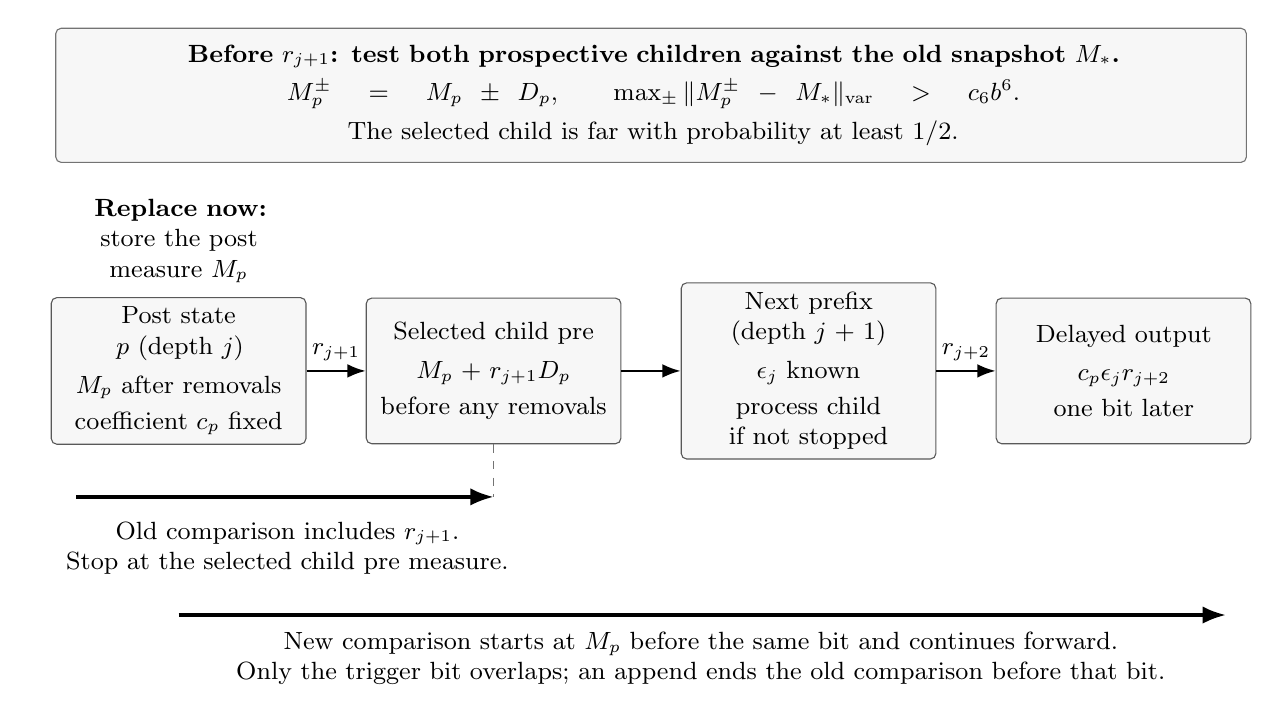
\begin{tikzpicture}[
  x=1cm,y=1cm,>=Latex,
  state/.style={draw=black!65,rounded corners=2pt,fill=black!3,
    text width=3cm,minimum height=1.85cm,align=center,font=\small},
  every node/.style={font=\small},
  comparison/.style={very thick,>=Latex}
]
  \node[draw=black!55,rounded corners=2pt,fill=black!3,
    text width=14.7cm,align=center,inner sep=6pt] at (6,5.1)
    {\textbf{Before $r_{j+1}$: test both prospective children against the old snapshot $M_*$.}\\[3pt]
     $M_p^\pm=M_p\pm D_p,\qquad
       \max_{\pm}\|M_p^\pm-M_*\|_{\rm var}>c_6b^6$.\\[3pt]
     The selected child is far with probability at least $1/2$.};

  \node[align=center,text width=3.6cm] at (0,3.25)
    {\textbf{Replace now:}\\store the post measure $M_p$};
  \node[state] (post) at (0,1.6)
    {Post state $p$ (depth $j$)\\[3pt]
     $M_p$ after removals\\[2pt]
     coefficient $c_p$ fixed};
  \node[state] (prechild) at (4,1.6)
    {Selected child pre\\[3pt]
     $M_p+r_{j+1}D_p$\\[2pt]
     before any removals};
  \node[state] (postchild) at (8,1.6)
    {Next prefix (depth $j+1$)\\[3pt]
     $\epsilon_j$ known\\[2pt]
     process child if not stopped};
  \node[state] (output) at (12,1.6)
    {Delayed output\\[3pt]
     $c_p\epsilon_j r_{j+2}$\\[2pt]
     one bit later};

  \draw[->,thick] (post.east) -- node[above] {$r_{j+1}$} (prechild.west);
  \draw[->,thick] (prechild.east) -- (postchild.west);
  \draw[->,thick] (postchild.east) -- node[above] {$r_{j+2}$} (output.west);

  \draw[dashed,black!55] (prechild.south) -- (4,0);
  \draw[comparison,->] (-1.3,0) -- (4,0);
  \node[align=center,text width=6.3cm,fill=white,inner sep=2pt] at (1.35,-0.65)
    {Old comparison includes $r_{j+1}$.\\Stop at the selected child pre measure.};

  \draw[comparison,->] (0,-1.5) -- (13.3,-1.5);
  \node[align=center,text width=13.2cm] at (6.6,-2.05)
    {New comparison starts at $M_p$ before the same bit and continues forward.\\
     Only the trigger bit overlaps; an append ends the old comparison before that bit.};
\end{tikzpicture}

 \caption{A distance trigger without an append. At the post state $p$, both
 child pre measures are compared with the old snapshot $M_*$. The snapshot
 is replaced by $M_p$ before $r_{j+1}$ is read. The old comparison includes
 that bit and ends at the actual child pre measure; the new comparison
 starts at $M_p$, so this bit is used twice at most. Any child removals occur
 afterward. The coefficient of the jump from $p$ is emitted using the
 delayed sign $r_{j+2}$, even if no child jump is made. Here $c_p$ denotes
 that fixed normalized transform coefficient. An append instead ends the old comparison before
 $r_{j+1}$, in its old coordinates.}
 \label{fig:07-snapshot-timing}
\end{figure}

On one comparison interval let $k$ be each removed positive joint mass
measure, expressed in its fixed coordinate space. Retain $k$ unchanged
after its removal and let $K$ be the sum retained so far. Then
\[
 N=M+K
\]
is a positive measure martingale under the uniform output bits. At a kill,
$M$ loses precisely the measure added to $K$. At a spatial bit its two
values are $N\pm D_{\rm jump}$, with
$|D_{\rm jump}|\le M\le N$. In particular the martingale starts from the
snapshot measure $M_*$, and all later measures are absolutely continuous
with respect to $M_*$: a zero coordinate set remains zero under positive
child averaging and removals.

Use generalized relative entropy for finite measures,
\[
 \mathcal E(N\mid M_*)=
       \int(n\log n-n+1)\,dM_*,\qquad n=dN/dM_*.
\]
At a spatial bit, writing $t=D_{\rm jump}/N$, its average increment is
\[
 \int \frac N2\bigl((1+t)\log(1+t)+(1-t)\log(1-t)\bigr)
 \le C\int\frac{|D_{\rm jump}|^2}{N}
 \le C\int\frac{|D_{\rm jump}|^2}{M}.
\]
The scalar ratio in this inequality is bounded on $-1\le t\le1$, with
its limit at zero understood. Kills leave $N$ unchanged. Bounded stopping
in the finite-depth tree therefore bounds the expected terminal entropy
by the expected Fisher sum on the comparison interval.

At a distance trigger, one of the two prospective children differs from
$M_*$ by more than $c_6b^6$, so the selected child has this property with
conditional probability at least one half. On that event either
$\|K\|\ge c_6b^6/2$, or
$\|N-M_*\|_{\rm var}>c_6b^6/2$. On the complementary event $\|K\|<c_6b^6/2$, the latter alternative
holds, $N$ has mass at most $4+c_6b^6/2$, and $M_*$ has mass at most two. The scalar inequality
\[
 \frac{(x-1)^2}{1+x}\le C(x\log x-x+1),\qquad x\ge0,
\]
followed by Cauchy--Schwarz gives
\[
 \|N-M_*\|_{\rm var}^2
 \le C\bigl(N(\Omega)+M_*(\Omega)\bigr)\mathcal E(N\mid M_*),
\]
where $\Omega$ is the fixed observation space of the comparison interval.
Thus the latter event forces
$\mathcal E(N\mid M_*)\ge c b^{12}$. Conditional on the comparison start,
the probability that its next replacement is a distance trigger is at most
\begin{equation}\label{eq:07-trigger-charge}
 C\mathbb E\left[
       b^{-6}\sum_{\rm interval}\xi_p
       +b^{-12}\sum_{\rm interval}
                      \int\frac{|D_{\rm jump}|^2}{M}
             \,\middle|\,\text{comparison start}\right].
\end{equation}
Indeed the far-child event has at least half the trigger probability, and
the preceding deterministic alternatives charge it to removals or to
terminal entropy, whose expectation was just bounded.

Sum \Cref{eq:07-trigger-charge} with the probabilities of the starts.
Every jump is in at most two comparison intervals: at a distance trigger
it is the final bit of the old interval and the first bit of the new one.
Appends stop old comparisons before their jump. Removals likewise have
bounded overlap. By \Cref{eq:07-kill-bounds,eq:07-rounded-fisher}, distance
triggers contribute the last two terms in
\Cref{eq:07-snapshot-count}. Initialization contributes at most one, and
append replacements at most $D_{\max}$. This proves the count. No coordinate
is re-observed merely because a snapshot is replaced, and the conditional
argument did not condition on a realized side or rounded value.
\end{proof}

\subsection{Activation and the one block of missed jumps}

\begin{lemma}[Activation and localization before activation]
\label{lemma:07-activation}
On a capped scheme, declare a high $u$ activated at a jump $p$ if there is
$v\in[D]$ such that $|u-v||p|\le\sigma$ in the main case, or
$|u-v||p|\le c_8b^4$ in the scalar case. A representative from the current
snapshot then gives the fixed decompositions and bounds in
\Cref{prop:capture}. All non-bad high jumps before first activation lie in
one block of at most $H_b$ depths as stated there.
\end{lemma}

\begin{proof}
Freeze the spatial phase $\chi_{u-v}$ at any point of $p$. The normalized
scalar error on a prospective child is at most $C|u-v||p|$, by its mass
bound. In the main case conditional Cauchy--Schwarz gives
\[
 \left|\sqrt{G_{p'}^u}-\sqrt{G_{p'}^v}\right|
 \le\left(\frac1\alpha\mathbb E_{p'}
       [a|\chi_{u-v}(Y)-\chi_{u-v}(y_p)|^2]\right)^{1/2}
 \le C|u-v||p|.
\]
Thus $v$ is high at $0.9b$, since $\sigma\ll b_0$ and the scalar
prefactor is small. By \Cref{lemma:07-snapshots}, it is covered by a stored
$s$. If that snapshot was born at $q\supseteq p$, its main cover gives
$v-s=n+j$, with $\Delta_A(n)\le r_{\rm sep}$ and $|j||q|\le\sigma$.
Set $a'=u-v+j$. Then $|a'||p|\le2\sigma$. The channel $A$ is fixed
throughout the plateau, so $n$ retains its metric bound. The scalar cover
instead gives $|v-s||q|\le c_7b^4$, and hence
$|(u-v)+(v-s)||p|\le(c_7+c_8)b^4$. Fix this $s,n,a'$ at activation;
all their spatial error bounds only improve on descendants.

Now let $p_0$ be the first non-bad high jump before any activation, if one
exists. By \Cref{eq:source-14} there is a signed combination $v\in[D]$ at
that node with
\[
 |u-v||p_0|\le P(D_{\max},d_1,1/b)
\]
for a fixed polynomial $P$. The same signed combination remains available
as the list grows. After $r$ further depths the left side with the new
interval is at most $2^{-r}P(D_{\max},d_1,1/b)$. For
\[
 r\ge C\log(CD_{\max}d_1/b)+C\log(1/\sigma)
\]
this is at most the relevant activation tolerance, $\sigma$ or $c_8b^4$.
Any subsequent high jump then activates, whether or not it is bad. Hence
every non-bad high jump strictly before first activation lies in the one
depth block beginning at $p_0$ of the claimed length. If no such $p_0$
exists there is no missed non-bad high jump. This proves the assertion and
completes \Cref{prop:capture}.
\end{proof}

The cap has been deterministic throughout the probability estimates. In
\Cref{sec:paths} the estimates will first be made simultaneous over all
dyadic caps, after which a cap comparable to $1+|D|_{\rm final}$ may be
selected on each path. In particular \Cref{eq:07-append-budget} and Jensen
give
\[
 \mathbb E_{\mathbf U_e}\log(C(1+|D|_{\rm final}))
       \le C\log(Cd_1/b),
\]
so this later choice incurs a logarithmic expected cost and excludes no
large-list paths.

\section{Delayed transforms along a plateau path}
\label{sec:paths}

The representatives from \Cref{sec:capture} will be used on intervals of
depths chosen while estimating an actual modulation. We therefore prove
interval bounds under explicit amplitude conditions, then make the bounds
simultaneous over all snapshot representatives and dyadic list caps.
Scalar moments handle small amplitudes and static plateaus; moments that
retain the main label handle the main levels on live plateaus.

Fix a plateau $e$, with normalization $\alpha=\alpha_e$, and use uniform
probability $\mathbf U_e$ on its root.  Write $\mathcal F_j$ for the spatial
prefix through depth $j$, together with the deterministic processing data at
that prefix.  In particular, every post state, its two prospective pre-child
states, and the decision to retain its jump are $\mathcal F_j$-measurable.
The sign $r_{j+1}$ is independent and fair conditional on $\mathcal F_j$.
The multiplier $\epsilon_j$ satisfies $|\epsilon_j|\le1$ and is
$\mathcal F_{j+1}$-measurable.  It is the same for every label coordinate.
Thus a coefficient formed at depth $j$ has its output multiplied by the
later sign $r_{j+2}$.  The additional bit allowed in the finite model supplies
this sign even for the final contributing jump.

All moments below are divided by $\alpha$.  At a jumping post state the
total mass is at most $2$, and at either prospective pre-child it is at
most $4$.  Intervening removals have normalized masses $\xi_p$; full removal
at an exit can be included.  We write $K_e=\sum_p\xi_p$ for the sum along
the entire plateau path.  These quantities and the local budget statements
are those of \Cref{lemma:07-local-budget}.  No realized input membership or
noisy label is sampled on this uniform output path.
All statements use the sufficiently large $d$ convention already fixed;
their constants are uniform in the finite spatial depth and in every
integer-frequency cutoff.

\subsection{The predictable sign inequality}

We use the standard exponential-supermartingale proof of a maximal
inequality, based on Ville's stopping argument
\cite[Chapter~V, first section, Theorem~1, pp.~84--85]{Ville1939}.
The finite-depth version below also records the conditional and
predictable-masking forms required later.

\begin{lemma}[Predictable signs]
\label{lemma:paths-sign}
Let $(r_{i+1})$ be fair signs in a filtration $(\mathcal F_i)$, and let
$c_i$ be real $\mathcal F_i$-measurable coefficients.  For every $\theta>0$
and $t\ge0$, outside an event of probability at most $e^{-t}$,
\[
 \sum_{i<n}c_i r_{i+1}
 \le \frac{\theta}{2}\sum_{i<n}c_i^2+\frac{t}{\theta}
 \qquad\text{for every prefix }n.
\]
The same statement holds conditionally at a stopping-time origin and with
predictable stopping or masking of the coefficients.  For complex sums one
may apply the assertion to both signs of each real component, at a total
failure probability at most $4e^{-t}$.
\end{lemma}

\begin{proof}
The elementary inequality $\cosh x\le e^{x^2/2}$ shows that
\[
 \exp\left(\theta\sum_{i<n}c_i r_{i+1}
                  -\frac{\theta^2}{2}\sum_{i<n}c_i^2\right)
\]
is a nonnegative supermartingale starting at one.  Stop at the first
crossing of $e^t$ to obtain the asserted maximal inequality.  Everything
is in finite depth, so optional sampling needs no limiting argument.
Starting the same calculation with conditional expectation given the
origin proves the conditional assertion.  Predictable masks are absorbed
in $c_i$.
\end{proof}

\subsection{Scalar moments and their masked transforms}

\begin{proposition}[Scalar plateau paths]
\label{prop:scalar-path}
Let $0<b\le1$ be a scalar level, and let $s$ be a representative selected at
a predictable snapshot birth on a live or static plateau.  At a jumping
post state put
\[
 f_p=\frac{\mathbb E_p[a\chi_s]}{\alpha},\qquad
 u_p=\frac{f_{p,+}-f_{p,-}}2,\qquad
 \eta_p=\mathbf1_{\{\max(|f_{p,+}|,|f_{p,-}|)\le C_3b\}},
\]
where $C_3$ is a fixed constant and $f_{p,\pm}=f_p\pm u_p$ are prospective
pre-child moments.  For every $t\ge0$, with conditional failure probability
at most $Ce^{-t}$ at the birth, every contiguous interval $I$ of subsequent
plateau jumps satisfies
\begin{equation}
 \left|\sum_{p\in I}\eta_p u_p\epsilon_{j(p)}r_{j(p)+2}\right|
 \le C b^{1/4}(1+K_e+t).
 \label{eq:source-15}
\end{equation}
Constants are independent of depth, $s$, and $b$; they may depend on the
fixed mask constant $C_3$.
\end{proposition}

\begin{proof}
Identify a complex moment with a point in $\mathbb R^2$ and set
\[
 \psi(x)=b^{1/2}\big((|x|^2+b^2)^{3/4}-b^{3/2}\big).
\]
On $|x|\le4$ one has $0\le\psi(x)\le Cb^{1/2}$ and
$|\nabla\psi(x)|\le Cb^{1/2}$.  More precisely,
\[
 \nabla^2\psi(x)
 =\frac32 b^{1/2}(|x|^2+b^2)^{-5/4}
       \left((|x|^2+b^2)\operatorname{Id}-\frac12 x x^{\mathsf T}\right).
\]
Its least eigenvalue is at least
$\frac34 b^{1/2}(|x|^2+b^2)^{-1/4}$.  Consequently it is at least
$c b^{1/2}$ throughout that ball, and at least $c(C_3)>0$ on
$|x|\le C_3b$.

Define the nonnegative averaging drift and the signed fluctuation by
\[
 \delta_p=\frac{\psi(f_p+u_p)+\psi(f_p-u_p)}2-\psi(f_p),\qquad
 n_p=\frac{\psi(f_p+u_p)-\psi(f_p-u_p)}2.
\]
Taylor's formula on the two segments $f_p\pm t u_p$, $0\le t\le1$, gives
\begin{equation}
 \delta_p\ge c b^{1/2}|u_p|^2,
 \qquad \delta_p\ge c(C_3)\eta_p|u_p|^2,
 \qquad n_p^2\le Cb|u_p|^2\le Cb^{1/2}\delta_p.
 \label{eq:paths-scalar-drift}
\end{equation}
For the second inequality the masked segment lies in the ball of radius
$C_3b$, since its endpoints do.  The last inequality follows from the
gradient bound and the first inequality.

At the actual pre-child the potential is exactly
$\psi(f_p)+\delta_p+r_{j+1}n_p$.  A removal of normalized mass $\xi$ changes
the complex moment by at most $\xi$, and hence changes $\psi$ by at most
$Cb^{1/2}\xi$.  Telescoping from birth to any prefix end therefore gives
\[
 \sum\delta_p\le Cb^{1/2}(1+K_e)-\sum r_{j+1}n_p.
\]
Apply \Cref{lemma:paths-sign} to the negative fluctuation with
$\theta=\gamma b^{-1/2}$, where $\gamma>0$ is a sufficiently small numerical
constant.  By \Cref{eq:paths-scalar-drift} its quadratic term is at most
$\frac12\sum\delta_p$.  Outside probability $e^{-t}$ this proves, on every
prefix,
\[
 \sum\eta_p|u_p|^2\le Cb^{1/2}(1+K_e+t).
\]
Now $\eta_pu_p\epsilon_j$ is known in $\mathcal F_{j+1}$ before $r_{j+2}$.
Apply \Cref{lemma:paths-sign} to the real and imaginary components of this
delayed transform with $\theta=b^{-1/4}$.  Their quadratic sums are bounded
by the preceding display.  Thus every prefix transform has absolute value
at most $Cb^{1/4}(1+K_e+t)$ except on probability $Ce^{-t}$.  Subtracting
the two prefixes bounding any contiguous interval proves
\Cref{eq:source-15}.  This subtraction retains precisely the fixed mask
$\eta_p$ within the interval.
\end{proof}

\subsection{The energy of label-valued moments}

For the main levels we need an $L^1(dz)$ estimate with an absolute
coefficient on the Fisher sum. This will let the assembly charge information
over disjoint intervals while paying separately for the choice of a
representative. The label norm controls the scalar transform because
integration against a label character recovers a shifted scalar modulation
multiplied by a thermal Fourier coefficient. The main representative is
chosen so that the coefficient needed in this recovery is close to one;
\Cref{sec:assembly} gives the exact decoding and the remaining spatial
phase error. We begin with the energy identities for the label-valued moments.

Fix a main representative $s$ on a live plateau, so its main channel $A$
is fixed. At a jumping post state $p$ with post density $a_p$, define
\[
 M(z)=\frac{\mathbb E_p[a_p(Y)K_A(z-Y)]}{\alpha},\qquad
 f(z)=\frac{\mathbb E_p[a_p(Y)\chi_s(Y)K_A(z-Y)]}{\alpha}.
\]
Here the observation consists only of the main label: the rounded
coordinates used to construct snapshots have been integrated out. Define
$M_\pm,f_\pm$ by the same formulas on the two prospective children, using
the same post density $a_p$. Write
\[
 f=Mv,\qquad f_\pm=M_\pm v_\pm,\qquad |v|,|v_\pm|\le1,
 \qquad D=\frac{M_+-M_-}2,\qquad \mathfrak a=\frac{f_+-f_-}2.
\]
The functions $v$ are set to zero at zero mass.  Define
\[
 G=\int M|v|^2\,dz,\qquad J=\int\frac{D^2}{M}\,dz,
 \qquad G_\pm=\int M_\pm|v_\pm|^2\,dz.
\]
In particular $J$ agrees with \Cref{eq:source-13}.  Quotients with zero
denominator are assigned zero; nonnegativity and child averaging make
their numerators zero as well.

\begin{lemma}[Energy drift and innovations]
\label{lemma:paths-innovation}
Put
\[
 g_z=\frac12\big(M_+|v_+-v|^2+M_-|v_--v|^2\big),\qquad
 g=\int g_z\,dz,\qquad U_p=\frac{G_+-G_-}2.
\]
Then
\begin{align}
 &g_z=\frac{M_+|v_+|^2+M_-|v_-|^2}{2}-M|v|^2\ge0,
       &|\mathfrak a-vD|^2&\le M g_z,\label{eq:paths-innovation-pointwise}\\
 &G_{\mathrm{actual\ pre}}=G+g+r_{j+1}U_p,
       &|U_p|^2&\le C\max(G_+,G_-)(J+g),\label{eq:paths-energy-noise}\\
 &&\left(\int|\mathfrak a|\,dz\right)^2&\le C(GJ+g).
       \label{eq:paths-moment-variation}
\end{align}
A removal of normalized mass $\xi$ changes $G$ in absolute value by at
most $3\xi$.  From any live jumping post state,
\begin{equation}
 \mathbb E\sum_{\mathrm{future}}g\le C,
 \qquad \mathbb E\sum_{\mathrm{future}}J\le Cd,
 \qquad \mathbb E\sum_{\mathrm{future}}\xi\le2,
 \label{eq:paths-forward-budgets}
\end{equation}
where the conditional law is spatially uniform on that state.
\end{lemma}

\begin{proof}
Child averaging gives
$M_+(v_+-v)=\mathfrak a-vD$ and $M_-(v_--v)=-(\mathfrak a-vD)$.  Expansion around $v$ proves the
first identity.  If both child masses are positive, it also gives
\[
 g_z=\frac{M|\mathfrak a-vD|^2}{M^2-D^2}.
\]
This implies the innovation inequality.  If a child mass is zero, the
corresponding moment is zero and $\mathfrak a-vD=0$, giving the same inequality.
Write $e=\mathfrak a-vD$.  Expanding the difference of the two child energies yields
\[
 U_p=\int D|v|^2\,dz+2\operatorname{Re}\int\overline v e\,dz+R,
 \qquad |R|\le g.
\]
Cauchy--Schwarz bounds the first two integrals in absolute value by
$\sqrt{GJ}$ and $\sqrt{Gg}$, respectively.  Since
$G+g=(G_++G_-)/2\le\max(G_+,G_-)$, squaring proves
\Cref{eq:paths-energy-noise}.  The decomposition $\mathfrak a=vD+e$ gives
\[
 \int|\mathfrak a|\,dz\le\sqrt{GJ}+\sqrt{\left(\int M\,dz\right)g}
                  \le\sqrt{GJ}+\sqrt{2g},
\]
which proves \Cref{eq:paths-moment-variation}.

For the removal assertion, the energy has the variational expression
\[
 \int\frac{|f|^2}{M}\,dz
 =\sup_{|\gamma(z)|\le1}
       \int\big(2\operatorname{Re}(\overline\gamma f)-|\gamma|^2M\big)\,dz.
\]
Removing $k_M\ge0$ and $k_f$ with $|k_f|\le k_M$ changes every test in this
supremum by at most $3\int k_M=3\xi$.  Both the old and new moment-to-mass
ratios have modulus at most one, so the same test class represents both
energies.  Finally telescope \Cref{eq:paths-energy-noise} over the entire
future stopped plateau path.  Its martingale terms have zero conditional
expectation, its terminal pre energy is at most $4$, and the removals have
expected total at most $2$.  This gives the first bound in
\Cref{eq:paths-forward-budgets}.  The other two are
\Cref{lemma:07-local-budget}.
\end{proof}

\subsection{A vector estimate on an outer-valid run}

For a main dyadic level $b\in[b_0,1]$, declare a jump exceptional when
$b<1$ and it is bad for the \emph{main} criterion at level $2b$.  Put
\[
 e'_p=C b_0^{-2}e_{p,2b}\mathbf1_{\{p\text{ exceptional}\}}
       \quad(b<1),\qquad e'_p=0\quad(b=1).
\]
Choose $C$ so that $e'_p\ge1$ on every exceptional jump; this is possible
because a bad main jump has edge mass at least $c(2b)^2$.  Let
$E_{e,b}=\sum_p e'_p$ on the whole plateau path.  Fix a sufficiently large
numerical $C_4$.  For the specified $s,b$, call a jump \emph{inner-valid}
if it is exceptional or $\max(G_+,G_-)\le C_4b^2$, and \emph{outer-valid}
if it is exceptional or $\max(G_+,G_-)\le2C_4b^2$.  At $b=1$ choose $C_4$
large enough that every jump is inner-valid.

\begin{lemma}[Drift on a run]
\label{lemma:paths-run-drift}
Start predictably at an outer-valid jump, and stop before the first
outer-invalid jump or at plateau end.  For $t\ge0$, outside conditional
probability $e^{-t}$, every prefix $P$ of this run satisfies
\begin{equation}
 \sum_{p\in P}g_p
 \le C\left(1+\sum_{p\in P}\xi_p+\sum_{p\in P}e'_p\right)
       +Cb\sum_{p\in P}J_p+Cb t.
 \label{eq:source-16}
\end{equation}
Removals here include those between consecutive jumps and may also be
enlarged to the whole plateau sum.
\end{lemma}

\begin{proof}
Telescope the exact energy identity of
\Cref{eq:paths-energy-noise}.  Initial and terminal energies are bounded
by $4$ and removals cost at most $3\xi$.  On an exceptional jump,
$|U_p|\le4\le4e'_p$, so pay its noise directly.  On the remaining jumps,
\Cref{eq:paths-energy-noise} gives
$|U_p|^2\le Cb^2(J_p+g_p)$.  Apply \Cref{lemma:paths-sign} to minus this
remaining noise with parameter $\theta=\gamma/b$.  Its quadratic bound is
$C\gamma b\sum(J_p+g_p)$.  Choose $\gamma$ small enough to absorb the
$g$ term, using $b\le1$.  Its other term is $Cb t$, which proves the
simultaneous prefix assertion.
\end{proof}

\begin{lemma}[Delayed norm estimate on a run]
\label{lemma:paths-run-norm}
Under the hypotheses of \Cref{lemma:paths-run-drift}, set
$\lambda=b^{1/2}$ and
$W_P(z)=\sum_{p\in P}\mathfrak a_p(z)\epsilon_{j(p)}r_{j(p)+2}$.  With conditional
failure probability at most $Ce^{-t}$, simultaneously for every run prefix,
\begin{equation}
 \int|W_P(z)|\,dz
 \le C\sum_{p\in P}J_p
      +C\lambda^{-1}\left(1+\sum_{p\in P}\xi_p+\sum_{p\in P}e'_p\right)
      +C\lambda t.
 \label{eq:source-17}
\end{equation}
In particular, the coefficient of the Fisher sum is absolute, independent
of $b$ and of the number of representatives.
\end{lemma}

\begin{proof}
We prove the norm estimate using both signs of a two-step block.  Separate
contributing depths into their two parities.  For one parity start at its
first depth in the run and group successive spatial jumps into blocks
$j,j+1$, with $j$ contributing to this parity.  Only complete blocks lying
in the prefix will be used in the norm telescope.  Denote the accumulated
transform for this parity at the block start by $W^{(0)}$, and put
\[
 X_0=(W^{(0)},f_0,\lambda M_0),\qquad
 \Phi=|X_0|=\big(|W^{(0)}|^2+|f_0|^2+\lambda^2M_0^2\big)^{1/2}.
\]
The complex coordinates are viewed as pairs of real coordinates.  Subscript
$0$ denotes the first post state.  After its sign $r=r_{j+1}$, write
$(\bar M,\bar f)$ for the actual pre-child, and $(M_1,f_1)$ for its post
state after removals $(k_M,k_f)$, where
\[
 \bar M=M_0+rD_0,\quad \bar f=f_0+r\mathfrak a_0,\quad
 M_1=\bar M-k_M,\quad f_1=\bar f-k_f,
 \quad k_M\ge0,\quad |k_f|\le k_M.
\]
Here and in this proof these are pointwise identities in $z$; in particular
$\int k_M=\xi_{j+1}$.  At the end of the second jump, before its child's
processing, the change in $X_0$ is exactly
\begin{equation}
 \Delta=\big(\mathfrak a_0\epsilon_jr',\;r\mathfrak a_0-k_f+r'\mathfrak a_1,
                    \lambda(rD_0-k_M+r'D_1)\big),\qquad r'=r_{j+2}.
 \label{eq:paths-two-step-increment}
\end{equation}

We first prove the required pointwise quadratic estimate.  Put
\[
 q=(|v_0|^2+\lambda^2)^{1/2},\qquad H=M_0q\le\Phi,
 \qquad j_i=\frac{D_i^2}{M_i},\qquad e_i=\mathfrak a_i-v_iD_i.
\]
For $M_0>0$, $q\ge\lambda$ and $|v_0|^2/q\le1$.  Positivity of the child
masses and of the removed density gives
\begin{equation}
 0\le M_1\le\bar M\le2M_0,
 \quad 0\le k_M\le\bar M\le2M_0,
 \quad |D_i|\le M_i,
 \quad |e_i|^2\le M_i g_{i,z}.
 \label{eq:paths-positive-domination}
\end{equation}
There is also a comparison of the child's post mean with the starting
mean:
\begin{equation}
                 M_1|v_1-v_0|^2\le4g_{0,z}+8k_M.
 \label{eq:paths-child-mean}
\end{equation}
To verify it, let $\bar v=\bar f/\bar M$ when $\bar M>0$, and zero otherwise.
The actual
child's term in the definition of $g_{0,z}$ gives
$\bar M|\bar v-v_0|^2\le2g_{0,z}$.  If $M_1=0$, the left side of
\Cref{eq:paths-child-mean} is zero.  If $0<M_1\le\bar M/2$, then
$M_1\le k_M$ and the bound $|v_1-\bar v|\le2$ gives
$M_1|v_1-\bar v|^2\le4k_M$.  If $M_1>\bar M/2$, the identity
\[
 M_1(v_1-\bar v)=k_M\bar v-k_f
\]
instead gives $M_1|v_1-\bar v|^2\le4k_M^2/M_1\le4k_M$, since $k_M<M_1$.
Thus the same bound covers every intermediate or arbitrarily small
remaining mass.  The squared triangle inequality, and $M_1\le\bar M$,
now prove \Cref{eq:paths-child-mean}.

Splitting $\mathfrak a_0=v_0D_0+e_0$ and retaining the factor $q$ yields
\begin{equation}
 \frac{|\mathfrak a_0|^2}{H}\le2j_0+\frac{2g_{0,z}}\lambda.
 \label{eq:paths-first-remainder}
\end{equation}
For the child jump use the three terms
$\mathfrak a_1=v_0D_1+(v_1-v_0)D_1+e_1$.  Their separate squared ratios obey
\begin{align*}
 \frac{|v_0D_1|^2}{H}&\le2j_1,\\
 \frac{|v_1-v_0|^2D_1^2}{H}
   &\le\frac{2}{\lambda}M_1|v_1-v_0|^2
       \le\frac{8g_{0,z}+16k_M}{\lambda},\\
 \frac{|e_1|^2}{H}&\le\frac{2g_{1,z}}\lambda.
\end{align*}
The factor $M_1/M_0\le2$ supplies the first and third bounds; the second
uses $|D_1|\le M_1$ and \Cref{eq:paths-child-mean}.  In particular no lower
bound on $M_1/M_0$ is used.  Hence
\begin{equation}
 \frac{|\mathfrak a_1|^2}{H}
 \le6j_1+\frac{24g_{0,z}+6g_{1,z}+48k_M}{\lambda}.
 \label{eq:paths-second-remainder}
\end{equation}
The mass-coordinate and removal terms satisfy
\[
 \frac{\lambda^2D_0^2}{H}\le j_0,
 \qquad \frac{\lambda^2D_1^2}{H}\le2j_1,
 \qquad \frac{k_M^2+|k_f|^2}{H}\le\frac{4k_M}{\lambda}.
\]
These follow again from \Cref{eq:paths-positive-domination} and
$0<\lambda\le1$.  If $M_0=0$, all the masses, half-differences, and
removals in \Cref{eq:paths-two-step-increment} are zero by positivity, so
$\Delta=0$ whether or not $W^{(0)}$ is zero.  This deals with every zero
denominator without an approximation argument.

For $\Phi>0$, concavity of the square root gives the global norm bound
\[
 |X_0+\Delta|\le\Phi+\left\langle\frac{X_0}{\Phi},\Delta\right\rangle
                              +\frac{|\Delta|^2}{2\Phi}.
\]
Combining the preceding pointwise inequalities and integrating proves
\begin{equation}
 \int\frac{|\Delta|^2}{2\Phi}\,dz
 \le C(J_0+J_1)+C\lambda^{-1}(g_0+g_1+\xi_{j+1}).
 \label{eq:paths-norm-remainder}
\end{equation}
The absolute Fisher coefficient results from the estimates of $v_0D_i$
with $q$, rather than replacing $q$ by $\lambda$ in those terms.

It remains to control the integrated linear term and its timing.  Write
$\Gamma_0=X_0/\Phi$, with value zero where $\Phi=0$.  Its norm is at most
one.  The linear term is
\[
 r L_0+r'L_1+L_{\rm kill},
\]
where $L_{\rm kill}$ has absolute value at most $2\xi_{j+1}$, and
$L_0,L_1$ are real integrated coefficients.  Specifically $L_0$ pairs
$\Gamma_0$ with $(0,\mathfrak a_0,\lambda D_0)$, whereas $L_1$ pairs it with
$(\mathfrak a_0\epsilon_j,\mathfrak a_1,\lambda D_1)$.  By
\Cref{eq:paths-moment-variation} and
$(\int|D_i|)^2\le(\int M_i)J_i\le2J_i$, their squares satisfy
\begin{equation}
 |L_0|^2+|L_1|^2
 \le C\sum_{i=0,1}\big((\lambda^2+G_i)J_i+g_i\big).
 \label{eq:paths-linear-variance}
\end{equation}

At a block start $W^{(0)}$ is $\mathcal F_j$-measurable: the previous
output of the same parity, if present, used $r_j$.  Thus $L_0$ is known
before $r_{j+1}$.  After that bit the removals, second post state, and
$\epsilon_j$ are all known, so $L_1$ is known before $r_{j+2}$.  Form one
scalar sign scheme by including $rL_0$ whenever the first jump is in the
run, and including $r'L_1$ only if the second jump is also in the run.
Both inclusion decisions are known before their respective signs.  The
linear sum through the last complete block of any prefix is itself a
prefix of this scheme.  If the run stops after a first step, no first
coefficient is retrospectively conditioned on the next validity decision.

On a nonexceptional included state $G_i\le2C_4b^2$.  At an exceptional
state both $G_i$ and $J_i$ are at most $2$, and $e'_i\ge1$.  Therefore
\[
 G_iJ_i\le Cb^2J_i+Ce'_i.
\]
Apply \Cref{lemma:paths-sign} to the linear scheme with parameter
$1/\lambda$.  Its quadratic term, by
\Cref{eq:paths-linear-variance}, is at most
\[
 C\sum J_p+C\lambda^{-1}\sum(g_p+e'_p),
\]
because $\lambda=b^{1/2}$ and $b\le1$.  The tail term is $\lambda t$.
All sums here can be restricted to the complete blocks of the prefix.
At the first block $W^{(0)}=0$ and $\int\Phi\le C$.  Between complete
blocks, passing from a pre state to the next post state changes the
integrated norm by at most $2\xi$, by the norm's Lipschitz property.
Telescoping, using \Cref{eq:paths-norm-remainder}, proves for the completed
blocks the bound
\[
 C\sum J_p+C\lambda^{-1}\left(1+\sum\xi_p+\sum e'_p+\sum g_p\right)
                              +C\lambda t.
\]
At most one contributing output of this parity is unmatched at a prefix
end.  It costs at most $\int|\mathfrak a_p|\le\int M_p\le2$, even if its delayed
sign occurs after the run has stopped.  Add this output directly.
The other parity is started conditionally on reaching its first jump,
one step later if necessary, and obeys the same bound with the same
conditional failure estimate.  Each prefix jump is used in at most two
of the completed-block estimates.  Finally apply
\Cref{eq:source-16} on this prefix.  Its $g$ contribution becomes
$C\lambda^{-1}(1+\sum\xi+\sum e')+C(b/\lambda)\sum J+C(b/\lambda)t$.
Since $b/\lambda=\lambda\le1$, adding the two parity bounds gives
\Cref{eq:source-17}.
\end{proof}

\subsection{Predictable runs and Fisher checkpoints}

The run estimate charges the Fisher sum from its origin. Subtracting two
prefixes to estimate a later interval would therefore charge the earlier
part of the run twice. We introduce predictable checkpoints so that this
extra Fisher charge is bounded by an absolute constant.

\begin{proposition}[Vector estimates on arbitrary inner-valid intervals]
\label{prop:vector-path}
Fix a live plateau, a main level $b\in[b_0,1]$, and a representative $s$
at its snapshot birth.  There is a family of predictable estimate origins,
containing run starts and the checkpoints described below, whose
conditional expected size at the birth is at most
$P(d,b_0^{-1})$ for an absolute fixed polynomial $P$.
For every $t\ge0$, outside a conditional event of probability at most
$C P(d,b_0^{-1})e^{-t}$, every contiguous interval $I$ of inner-valid jumps
after this birth satisfies
\begin{equation}
 \int\left|\sum_{p\in I}\mathfrak a_p(z)\epsilon_{j(p)}r_{j(p)+2}\right|\,dz
 \le C\sum_{p\in I}J_p
       +Cb^{-1/2}(1+K_e+E_{e,b})+Cb^{1/2}t.
 \label{eq:paths-inner-interval}
\end{equation}
The Fisher sum is taken only over $I$.  The representative remains
eligible for these estimates until the plateau ends, even if another
snapshot has meanwhile replaced the one at which it was born.
\end{proposition}

\begin{proof}
Start a run at the first inner-valid opportunity after birth, possibly at
the birth jump itself.  Follow consecutive outer-valid jumps, stopping
before the first outer-invalid jump or at plateau end.  After a break,
start the next run at the first later inner-valid opportunity.  These are
predictable rules: both prospective child energies and the exceptional
indicator are known before the jump sign.  Every contiguous inner-valid
interval lies in one of these outer-valid runs.

We first bound the number of run starts conditionally on the birth
prefix.  A start on an exceptional jump can be charged to that jump.
\Cref{lemma:07-edge-charges} bounds the expected number of these by
$d\poly(h)$; there are none when $b=1$.  At a nonexceptional start,
$G_{\rm start}\le C_4b^2$.  If its run breaks, include the first invalid
jump in a comparison interval, although the transform estimate stops
before it.  At that jump $\max(G_+,G_-)>2C_4b^2$.  Conditional on the
prefix there, with probability at least $1/2$ its actual pre-child energy
exceeds $2C_4b^2$.  Mark such a break.  The comparison intervals for
different runs are disjoint, including their invalid jumps.

Let $Q$ denote one such start-to-break comparison interval, and put
$\mathcal M_Q=\sum_{p\in Q}r_{j(p)+1}U_p$.  By the exact energy identity
and the removal bound, a marked break implies
\[
 C_4b^2\le\sum_{p\in Q}g_p+3\sum_{p\in Q}\xi_p+|\mathcal M_Q|.
\]
Consequently, with a numerical constant depending only on $C_4$,
\begin{equation}
 \mathbf1_{\{Q\text{ marked}\}}
 \le Cb^{-2}\sum_{p\in Q}(g_p+\xi_p)+Cb^{-4}|\mathcal M_Q|^2.
 \label{eq:paths-marked-break}
\end{equation}
To use orthogonality, first include every start-to-break interval of this
type and the possible unfinished terminal interval, without conditioning
on a mark.  Its starting rule and inclusion through the invalid bit are
predictable.  Thus stopped martingale orthogonality gives
\[
 \mathbb E\sum_Q|\mathcal M_Q|^2
 =\mathbb E\sum_{p\in\bigcup Q}U_p^2
 \le C\mathbb E\sum_p(J_p+g_p),
\]
using \Cref{eq:paths-energy-noise} and $\max(G_+,G_-)\le4$.  All
expectations here are conditional at birth.  Each nonexceptional break
is marked with conditional probability at least $1/2$, so
\Cref{eq:paths-marked-break,eq:paths-forward-budgets} imply
\[
 \mathbb E\#\{\text{nonexceptional-start runs that break}\}
 \le Cb^{-2}+Cdb^{-4}.
\]
At most one final run fails to break.  Including exceptional starts
proves a bound $P(d,b_0^{-1})$ for all starts, uniformly in $s$.  The
factor $\poly(h)$ is absorbed in a fixed power of $b_0^{-1}$.

Within each outer-valid run, also start an estimate whenever the
accumulated $J$ since the preceding origin reaches one.  More precisely,
after including the jump that reaches this threshold, reset the counter
and use the next jump as a new origin if it remains in the run.  Each
such origin's estimate continues to that run's same break or end.  The
counter decision is known at this next origin; no future bit is used.
The number of additional origins is at most the total $J$ of the path,
and $J_p\le\int M_p\le2$ bounds a threshold overshoot.  Therefore their
conditional expected number is at most $Cd$ by
\Cref{eq:paths-forward-budgets}.

Apply \Cref{lemma:paths-run-norm} conditionally at every origin, with the
same parameter $t$.  Summing its conditional failure probabilities
weights each origin by its probability of being reached.  The expected
origin count just proved bounds the resulting probability by
$C P(d,b_0^{-1})e^{-t}$.
On the event of simultaneous success, fix any desired interval $I$ and
choose the latest origin $q$ in its outer-valid run at or before its first
jump.  The total $J$ between $q$ and that first jump is at most $3$;
indeed the counter is below one before a threshold crossing, and one
jump adds at most two.  The interval transform is the difference of
two prefixes from $q$.  Their Fisher sums add to
\[
 \sum_{p\in I}J_p+2\sum_{q\le p<\min I}J_p
 \le\sum_{p\in I}J_p+6.
\]
Their removal and exceptional sums are bounded by twice $K_e$ and
$E_{e,b}$, respectively.  The extra constant is absorbed by
$b^{-1/2}(1+K_e+E_{e,b})$.  The triangle inequality in $L^1(dz)$ then
proves \Cref{eq:paths-inner-interval}.  This argument also permits the
interval to begin long after the snapshot's replacement.
\end{proof}

\subsection{Simultaneous representatives and random list caps}

\begin{lemma}[Parameters for all representatives at a level]
\label{lemma:paths-simultaneous}
On each plateau and at each permitted level there are nonnegative random
parameters $t_b,H_b$, independent of the actual frequency later being
estimated, with the following properties.  Almost surely the scalar
bound of \Cref{prop:scalar-path}, or the vector interval bound of
\Cref{prop:vector-path}, holds with $t=t_b$ for every representative in
the snapshot construction used on the path.  The activation conclusion
of \Cref{lemma:07-activation} holds with miss-block length $H_b$.
Moreover
\begin{align}
 \mathbb E_{\mathbf U_e}t_b
   &\le Ck_{b/4}+C\log(Cd/b) &&\text{for main levels},
       \label{eq:paths-main-parameter}\\
 \mathbb E_{\mathbf U_e}t_b
   &\le C\big(d_1+\log(1/b)\big) &&\text{for scalar levels},
       \label{eq:paths-scalar-parameter}\\
 \mathbb E_{\mathbf U_e}H_b
   &\le C\log(Cd_1/b)+C\log(1/\sigma)
       &&\text{for either criterion}.
       \label{eq:paths-miss-parameter}
\end{align}
These assertions hold simultaneously over the countably many levels.
\end{lemma}

\begin{proof}
Begin with a deterministic dyadic cap $D_{\max}=2^m$, $m\ge0$.
The broad list is constructed independently of this cap.  The capped
snapshot scheme creates snapshots only while its list length is at most
$D_{\max}$; estimates for representatives already born continue to the
plateau end.  By \Cref{lemma:07-snapshots}, the expected number of births
is bounded by a fixed polynomial in $(D_{\max},d_1,1/b)$.  The number of
representatives in each snapshot is at most
\[
 R_b^{\rm main}=\lceil e^{k_{b/2}}\rceil,
 \qquad R_b^{\rm sc}=\exp\big(C(d_1+\log(1/b))\big),
\]
as established in that lemma.  Scalar estimates originate at these
births.  For each main representative, \Cref{prop:vector-path} bounds
the conditional expected number of run and checkpoint origins by a
fixed polynomial in $(d,b_0^{-1})$.  For sufficiently large $d$ this
factor is also bounded by a fixed power of $d$, because
$b_0^{-1}\le2h^{16}\le d$.

Here is the conditional union argument, which also applies when the
number of origins is random.  Enumerate predictable origins by their
finite tree addresses and, within an address, by their representative
indices.  If $B_o$ is the event that origin $o$ is reached and an estimate
starting there fails with deterministic parameter $t$, then
\[
 \mathbb P(B_o)
 \le Ce^{-t}\mathbb P(o\text{ is reached}).
\]
Sum this inequality over origins and then use their expected count.
Thus the failure probability for a capped scheme is at most $Ce^{-t}$
times its stated representative cardinality and polynomial count.  No
union over the signed span of the broad list is taken.

Choose sufficiently large fixed constants and define baseline parameters
\[
 T_b^{\rm main}=Ck_{b/4}+C\log(Cd/b),\qquad
 T_b^{\rm sc}=C(d_1+\log(1/b)).
\]
They absorb the logarithms of the representative cardinalities and all
polynomial factors except the cap.  For a sufficiently large further
fixed $C_{\rm cap}$, use
\[
 t=T_b+C_{\rm cap}\log(CD_{\max})+z
\]
in each deterministic capped scheme.  Its failure probability is at most
$C2^{-2m}e^{-z}$, after increasing $C_{\rm cap}$ if necessary.  Summing
over all dyadic caps gives $Ce^{-z}$.  These events are nested as $z$
increases, since every right-hand side in the path estimates increases.
Let $Z_b$ be the least nonnegative integer $z$ for which all these capped
schemes succeed.  Integer tail summation gives
\[
 \mathbb P(Z_b>n)\le Ce^{-n},\qquad \mathbb E Z_b\le C,
\]
and $Z_b$ is finite almost surely.

Only now choose a cap from the realized output path: let
$\widehat D$ be the least dyadic integer at least
$1+|D|_{\rm final}$ for the broad list at this level.  Thus
$1+|D|_{\rm final}\le\widehat D<2(1+|D|_{\rm final})$, and its capped
scheme never breaches the cap on this path.  The simultaneous assertion
over deterministic caps permits this selection without a stopping-time
claim about $\widehat D$.  Set
\[
 t_b=T_b+C_{\rm cap}\log(C\widehat D)+Z_b.
\]
Broad capture gives $\mathbb E|D|_{\rm final}\le Cd_1b^{-C}$, so Jensen's
inequality yields
\[
 \mathbb E\log(C\widehat D)
 \le C+\log\big(C(1+\mathbb E|D|_{\rm final})\big)
 \le C\log(Cd_1/b).
\]
This proves \Cref{eq:paths-main-parameter,eq:paths-scalar-parameter}, using
$d_1=d$ for main levels and $\log d_1\le d_1$ for scalar levels.
Use \Cref{lemma:07-activation} with this same cap and put
\[
 H_b=C\log(C\widehat Dd_1/b)+C\log(1/\sigma).
\]
Its expectation satisfies \Cref{eq:paths-miss-parameter}.  In the static
case the optional term $\log(1/\sigma)=40\log h$ is at most $Cd\le Cd_1$;
thus it causes no loss in the scalar plateau bound used below.

For each level the construction has a probability-one success event.
Their countable intersection still has probability one.  The resulting
parameters depend on the plateau path and the level, but not on the
integer frequency whose transform will be compared to these
representatives.
\end{proof}

\section{Assembly of the dyadic estimate}\label{sec:assembly}

We prove the modulated delayed Haar estimate stated in
\Cref{prop:dyadic}. First we bound the contribution of a single plateau,
using its representatives to recover each actual modulation. We then sum
these contributions with the plateau starting weights, keeping the
live Fisher and edge charges global.

\begin{proof}[Proof of \Cref{prop:dyadic}]
The zero input is immediate.  For positive input, apply the finite
procedure of \Cref{sec:procedure}, with the common stopping rule in the
statement.  In particular, the cutoff always refers to the original
$\rho$, including when a subpiece is being processed.  The parameter
constants are fixed in the order specified there, and $d_0$ is increased
to satisfy their finitely many large-$d$ requirements.

\subsection*{The contribution of one plateau}

For a plateau $e$, write $p_e$ for its root, $\alpha_e$ for its
normalization, and $\mathbf U_e$ for uniform probability on $p_e$.
On an output path $x\in p_e$, let $\mathcal P_e(x)$ be its consecutive
jumping nodes belonging to this plateau.  The post density at a node
$p\in\mathcal P_e(x)$ is denoted by $a_p$.  Thus all removals at $p$
have already occurred, and $a_p$ is the density whose two prospective
child moments are used in that jump.  In sums over nodes $p$, write
$j=\operatorname{depth}(p)$.  Define
\[
 c_p^u=\frac1{\alpha_e}\E_p[a_p(Y)\chi_u(Y)r_{j+1}(Y)],
 \qquad
 \mathcal T_e^u(x)=\sum_{p\in\mathcal P_e(x)}
           c_p^u\epsilon_j(x)r_{j+2}(x).
\]
At each jumping node the post pieces partition the original density.
Consequently their transforms satisfy the exact identity
\[
 \mathcal H_{I,J}^{u}\rho(x)
    =\sum_{e:\,x\in p_e}\alpha_e\mathcal T_e^u(x).
\]
Put $w_e=\mathbf U(p_e)\alpha_e$. The triangle inequality and integration
with respect to $\mathbf U$ give
\begin{equation}\label{eq:09-plateau-reduction}
 \int_I\max_{\substack{u\in\mathbb Z\\|u|\le Q}}
       |\mathcal H_{I,J}^{u}\rho|\,d\mathbf U
 \le\sum_e w_e\mathbb E_{\mathbf U_e}
                     \sup_{u\in\mathbb Z}|\mathcal T_e^u|.
\end{equation}
We will bound this weighted sum by $Cd$, charging the live Fisher and
edge terms across all pieces and the remaining terms one plateau at a time.

The local mass bound gives $|c_p^u|\le2$ and prospective child masses
at most $4$, in this normalization.  Let $K_e(x)$ denote the sum of all
normalized removal masses $\xi_p$ on the plateau's processing path,
including the intervening and terminal removals allowed in
\Cref{prop:capture}; then
\begin{equation}\label{eq:09-kills}
 \E_{\mathbf U_e}K_e\le1.
\end{equation}
For live plateaus set $d_1=d$, and for static plateaus set
$d_1=d+2+\log^-\alpha_e$.

Use the main levels
$\mathcal B_{\rm m}=\{2^{-j}:b_0\le2^{-j}\le1\}$ on live plateaus.
Use scalar levels
$\mathcal B_{\rm s}(B)=\{B2^{-j}:j\ge0\}$, where $B=b_0$ on a live
plateau and $B=1$ on a static plateau.  At the shared level $b_0$ the
main and scalar constructions are distinct.  By
\Cref{lemma:paths-simultaneous}, they have nonnegative, frequency-independent
path parameters $t_b^{\rm m},t_b^{\rm s}$ and miss-block lengths
$H_b^{\rm m},H_b^{\rm s}$, satisfying
\begin{align}
 \E_{\mathbf U_e}t_b^{\rm m}
   &\le C k_{b/4}+C\log(Cd/b),
       &&b\in\mathcal B_{\rm m},\label{eq:09-main-parameters}\\
 \E_{\mathbf U_e}t_b^{\rm s}
   &\le C(d_1+\log(1/b)),
       &&b\in\mathcal B_{\rm s}(B),\label{eq:09-scalar-parameters}\\
 \E_{\mathbf U_e}H_b^{\rm m},\quad
 \E_{\mathbf U_e}H_b^{\rm s}
   &\le C\log(Cd_1/b)+C\log(1/\sigma)
       &&\text{for the levels where they are used.}
       \label{eq:09-miss-parameters}
\end{align}
These statements already include all snapshot births, representative
choices, starts, checkpoints, and dyadic list caps.  In particular we may
use the same parameters for every actual integer $u$.

At a live jumping piece write
\[
 E_{p,b}^{\rm m}=e_{p,b}\mathbf1_{\{p\text{ bad at main level }b\}}.
\]
For the scalar construction let $\bar b(p)$ be its largest bad level,
if there is one, and put
\[
 E_p^{\rm s}=e_{p,\bar b(p)}
 \quad\text{if a bad scalar level exists},\qquad E_p^{\rm s}=0
 \quad\text{otherwise}.
\]
A nonempty subset of the dyadic levels bounded above by $B$ has a
largest member.  This choice is determined by the jumping piece before
its bit and is independent of $u$.  The scalar edge regions are nested
as $b$ increases: their defining $l_b$ decreases.  Hence
\begin{equation}\label{eq:09-edge-monotonicity}
 b\le\bar b(p)\quad\Longrightarrow\quad e_{p,b}\le e_{p,\bar b(p)}.
\end{equation}

\subsection*{Main amplitudes and exact decoding}

Fix an integer $u$ and a live plateau path.  Starting with its first main
activation, including that jump, retain the largest main level activated
so far.  This level is nondecreasing.  Its positive intervals therefore
use each level $b$ at most once.  On the interval assigned to $b$, keep
the representative $s$ and decomposition supplied at its first
activation:
\begin{equation}\label{eq:09-main-decomposition}
 u=s+n+a',\qquad \Delta_A(n)\le r_{\rm sep},\qquad
 |a'|\,|p_{\rm act}|\le C\sigma.
\end{equation}
The form $A$ is fixed on this plateau.  All subsequent nodes in the
interval lie below $p_{\rm act}$.

For clarity, the comparison of criteria uses no loss depending on the
number of representatives.  For a prospective child $q$ of $p$, write
$f_q^v(z)=\alpha_e^{-1}\E_q[a_p(Y)\chi_v(Y)K_A(z-Y)]$ and
$M_q(z)=\alpha_e^{-1}\E_q[a_p(Y)K_A(z-Y)]$.
For the fixed output point $x\in p$, conditional Cauchy--Schwarz gives
\[
 \left\|f_q^u-\chi_n(\cdot)\chi_{a'}(x)f_q^s
       \right\|_{L^2(M_q^{-1}dz)}
 \le C\Delta_A(n)+C|a'|\,|p|.
\]
Indeed the square of the channel part is at most
\[
 \frac1{\alpha_e}\E_q\left[
     a_p(Y)\int |\chi_n(Y)-\chi_n(z)|^2K_A(z-Y)\,dz\right]
 =\frac{\E_q a_p}{\alpha_e}\Delta_A(n)^2,
\]
and the spatial part uses
$|\chi_{a'}(Y)-\chi_{a'}(x)|\le2\pi|a'|\,|p|$ and
$\E_q a_p/\alpha_e\le4$.  The triangle inequality in this weighted
Hilbert space proves
\begin{equation}\label{eq:09-criterion-comparison}
 \left|\sqrt{G_q^u}-\sqrt{G_q^s}\right|
 \le C(r_{\rm sep}+\sigma)\ll b_0\le b.
\end{equation}

If $b<1$, level $2b$ has not activated at any jump of this
interval.  Its non-bad high jumps before activation lie in one block of
at most $H_{2b}^{\rm m}$ depths, by \Cref{prop:capture}.  Remove the
intersection of that entire block with the current interval and pay
$C H_{2b}^{\rm m}$ directly, using $|c_p^u|\le2$.  The remaining jumps
form at most two contiguous intervals.  On each, a nonexceptional jump
is not high for $u$ at $2b$; thus
\Cref{eq:09-criterion-comparison} makes it inner-valid for $s,b$ in
\Cref{prop:vector-path}.  Here the exceptional jumps are precisely the
bad main jumps at $2b$.  When $b=1$, every jump is inner-valid after the
fixed constant in that definition is chosen large enough, since all
$G_q^s\le4$; no block is removed and no exception is needed.

We next verify the decoding of the vector estimate back to the actual
scalar modulation.  Put
\[
 \mathfrak a_p^s(z)
   =\frac1{\alpha_e}\E_p[a_p(Y)\chi_s(Y)r_{j+1}(Y)K_A(z-Y)],
 \qquad c_A(n)=\int\chi_n(\theta)K_A(\theta)\,d\theta.
\]
Evenness and positivity of the thermal Fourier coefficients imply
\begin{equation}\label{eq:09-decoding}
 c_A(n)=1-\tfrac12\Delta_A(n)^2\ge\tfrac12,
 \qquad
 \int\chi_n(z)\mathfrak a_p^s(z)\,dz=c_A(n)c_p^{s+n}.
\end{equation}
This is an exact identity, obtained by putting $z=Y+\theta$ in the
inner integral.  On any subset of the nodes below $p_{\rm act}$,
\[
 \sum_p|c_p^u-\chi_{a'}(x)c_p^{s+n}|
 \le C|a'|\sum_p|p|
 \le C|a'|\,|p_{\rm act}|\le C\sigma.
\]
The sum of lengths is geometric because the nodes lie on one descending
path.  The bound applies in particular to each retained subinterval.
Since the multipliers are common to all label coordinates,
\Cref{eq:09-decoding} now gives
\begin{equation}\label{eq:09-vector-to-scalar}
 \left|\sum_{p\in L}c_p^u\epsilon_jr_{j+2}\right|
 \le2\int\left|\sum_{p\in L}\mathfrak a_p^s(z)
                           \epsilon_jr_{j+2}\right|\,dz+C\sigma
\end{equation}
for every retained subinterval $L$.

Apply \Cref{prop:vector-path} to $L$.  Its Fisher sum is charged only
on $L$.  The intervals at distinct retained levels are disjoint, and
there are at most two retained subintervals at each level.  Thus these
Fisher charges have an absolute bounded multiplicity at every jumping
piece.  All kill and exceptional sums may use the whole plateau path.
Writing the exceptional proxy as
$e'_p=C b_0^{-2}E_{p,2b}^{\rm m}$, and using
$b^{-1/2}b_0^{-2}\le b_0^{-3}$ for $b\ge b_0$, we have bounded the whole
main part by a constant times
\begin{equation}\label{eq:09-main-path-bound}
 \sum_pJ_p+b_0^{-3}\sum_p\sum_{b\in\mathcal B_{\rm m}}E_{p,b}^{\rm m}
 +\sum_{b\in\mathcal B_{\rm m}}
       \left[b^{-1/2}(1+K_e)+b^{1/2}t_b^{\rm m}+H_b^{\rm m}\right].
\end{equation}
The constants in the vector estimates and the geometric decoding errors
are absorbed by the displayed $b^{-1/2}$ terms.

\subsection*{The scalar prefix and all static paths}

On a live plateau consider the prefix strictly before the first main
activation, or the whole path if no main activation occurs.  On a static
plateau consider the entire path.  Use the scalar levels through $B$
specified above, again retaining the largest activated level so far,
including activations at the current jump, and using zero if none has
activated.  There are finitely many changes
on this finite path even though the available scalar levels extend
arbitrarily close to zero.  Each positive level $b$ is retained on at
most one contiguous interval.

For its fixed representative $s$, scalar activation supplies
$u=s+a'$ with $|a'|\,|p_{\rm act}|\le Cb^4$, with the sufficiently
small constant in \Cref{prop:capture}.  On this level interval sum first
over the fixed scalar mask
\[
 \max\{|f_{p,+}^s|,|f_{p,-}^s|\}\le C_3b.
\]
This is precisely the masked transform in \Cref{prop:scalar-path}; that
proposition applies to the masked sum over the whole contiguous level
interval.  Freezing $\chi_{a'}$ at $x$ changes this masked sum by at most
$Cb^4$, by the same geometric sum of interval lengths as above.  Hence
all such masked sums cost at most
\begin{equation}\label{eq:09-scalar-mask-sum}
 C\sum_{b\in\mathcal B_{\rm s}(B)}b^{1/4}
                         (1+K_e+t_b^{\rm s}).
\end{equation}

Treat every remaining jump directly.  This includes all jumps while the
retained level is zero.  Put
$A'_p=\max\{|f_{p,+}^u|,|f_{p,-}^u|\}\le4$ in the unlabelled scalar
notation.  The direct jump costs at most $A'_p$, and a zero value needs
no charge.  If a positive level $b$ is currently retained, the jump is
outside its mask; the spatial phase comparison gives
$A'_p\ge C_3b-Cb^4>4b$, on taking $C_3$ large enough.

For a live prefix, any direct jump with $A'_p>4b_0$ is high at main
level $b_0$.  In fact $f_{p,\pm}^u=\int f_{p,\pm}^u(z)\,dz$ and
Cauchy--Schwarz gives
$|f_{p,\pm}^u|^2\le(\int M_{p,\pm})G_{p,\pm}^u\le4G_{p,\pm}^u$.
No main level has yet activated in this prefix.  All its non-bad main
high jumps at $b_0$ are therefore paid by its one miss block, and its
bad jumps are paid by
$C b_0^{-2}E_{p,b_0}^{\rm m}$, since each direct coefficient is at most
$4$.  These costs are already included, up to constants, in
\Cref{eq:09-main-path-bound}.

At every other nonzero direct jump we have $A'_p\le4B$; this holds
automatically on a static path with $B=1$.  Choose the largest available
scalar level $\widetilde b\le A'_p$.  Then
\[
 A'_p/4\le\widetilde b\le A'_p,
\]
and the jump is high at $\widetilde b$.  This level has not activated:
if the current level is positive, $A'_p>4b$ implies
$\widetilde b>b$, and otherwise none has activated.  All non-bad jumps
assigned to a fixed $\widetilde b$ consequently lie in its single
preactivation miss block and cost at most
$C\widetilde b H_{\widetilde b}^{\rm s}$ together.  If the assigned
level is bad, then
$e_{p,\widetilde b}\ge c\widetilde b$ and
\Cref{eq:09-edge-monotonicity} gives
\[
 A'_p\le4\widetilde b\le C e_{p,\widetilde b}\le C E_p^{\rm s}.
\]
Thus only one predictably selected scalar edge level per jump is
charged.  This establishes the scalar accounting for every positive
amplitude, including arbitrarily small amplitudes.

Combining these conclusions, the same frequency-independent quantity
bounds $\sup_u|\mathcal T_e^u|$ on a live plateau:
\begin{align}
 C^{-1}\sup_{u\in\Z}|\mathcal T_e^u|
 \le{}&\sum_{p\in\mathcal P_e(x)}
       \left(J_p+b_0^{-3}\sum_{b\in\mathcal B_{\rm m}}E_{p,b}^{\rm m}
                     +E_p^{\rm s}\right)\notag\\
 &+\sum_{b\in\mathcal B_{\rm m}}
       \left[b^{-1/2}(1+K_e)+b^{1/2}t_b^{\rm m}+H_b^{\rm m}\right]\notag\\
 &+\sum_{b\in\mathcal B_{\rm s}(b_0)}
       \left[b^{1/4}(1+K_e+t_b^{\rm s})+bH_b^{\rm s}\right].
       \label{eq:09-live-majorant}
\end{align}
For a static plateau the corresponding bound is
\begin{equation}\label{eq:09-static-majorant}
 \sup_{u\in\Z}|\mathcal T_e^u|
 \le C\sum_pE_p^{\rm s}
    +C\sum_{b\in\mathcal B_{\rm s}(1)}
       \left[b^{1/4}(1+K_e+t_b^{\rm s})+bH_b^{\rm s}\right].
\end{equation}
The path constructions and bounds used here hold simultaneously outside
one $\mathbf U_e$-null set.  The countable scalar-level sums have finite
expectation by the estimates below.  In particular no exceptional set
depending on the actual modulation is introduced in these majorants.

\subsection*{Summing levels and live weights}

Write $b_0=2^{-M}$, so $M=O(1+\log h)$.  Since
$k_b=A_0(d/h)(1+\log(1/b))^2$, the main cardinality tails satisfy
\begin{equation}\label{eq:09-main-series}
 \sum_{b\in\mathcal B_{\rm m}}b^{1/2}k_{b/4}
 =A_0\frac dh\sum_{j=0}^{M}2^{-j/2}
                          \bigl(1+(j+2)\log2\bigr)^2
 \le C\frac dh.
\end{equation}
The additional logarithms in \Cref{eq:09-main-parameters} sum to
$O(\log(Cd))$ with the same $b^{1/2}$ weights.  Also,
\[
 \sum_{b\in\mathcal B_{\rm m}}b^{-1/2}\E(1+K_e)
       \le Cb_0^{-1/2}\le Ch^8,
 \qquad
 \sum_{b\in\mathcal B_{\rm m}}\E H_b^{\rm m}
       \le C(1+\log h)\bigl(\log(Cd)+\log h\bigr).
\]
Every fixed polynomial in $h$, multiplied by $1+\log d$, is
$o(d/h)$ because $h=\log\log d$.  Thus the second line of
\Cref{eq:09-live-majorant} has expectation $O(d/h)$.

For the scalar series write $b=B2^{-j}$.  The convergent sums
$\sum_{j\ge0}2^{-j/4}$ and $\sum_{j\ge0}j2^{-j/4}$, together with
\Cref{eq:09-kills,eq:09-scalar-parameters,eq:09-miss-parameters}, give
\begin{align}
 &\sum_{b\in\mathcal B_{\rm s}(B)}
  \E\left[b^{1/4}(1+K_e+t_b^{\rm s})+bH_b^{\rm s}\right]\notag\\
 &\hspace{1cm}\le
 C B^{1/4}\bigl(d_1+1+\log(1/B)+\log(1/\sigma)\bigr).
 \label{eq:09-scalar-series}
\end{align}
For example the miss-block part alone is bounded by
$CB(\log(Cd_1/B)+\log(1/\sigma)+1)$, which is no larger than the
displayed right side.  On live plateaus $B=b_0\le h^{-16}$ and $d_1=d$,
so this is $O(d/h^4)$ and hence $O(d/h)$.  On static plateaus $B=1$ and
$d_1\ge d$, so $\log(1/\sigma)=40\log h\le Cd_1$ makes it $O(d_1)$.
The local scalar edge bound in \Cref{prop:capture} therefore proves
\begin{equation}\label{eq:09-static-plateau}
 \E_{\mathbf U_e}\sup_u|\mathcal T_e^u|\le C(d+2+\log^-\alpha_e)
 \quad\text{for every static plateau.}
\end{equation}

For every nonnegative jump quantity
$V_p$ of a plateau, change of the uniform root measure gives exactly
\begin{equation}\label{eq:09-weight-conversion}
 \sum_e w_e\E_{\mathbf U_e}\sum_{p\in\mathcal P_e(x)}V_p
   =\sum_{\text{jumping pieces }p}\mathbf U(p)\alpha_e V_p.
\end{equation}
The Fisher bound in \Cref{prop:live-budgets} bounds the right side by
$Cd$ when $V_p=J_p$ and $e$ is live.  The global scalar edge assertion
of \Cref{prop:capture} does the same for $V_p=E_p^{\rm s}$.  Its global
main edge assertion yields
\[
 b_0^{-3}\sum_{\text{live jumping pieces }p}
       \mathbf U(p)\alpha_e\sum_{b\in\mathcal B_{\rm m}}E_{p,b}^{\rm m}
 \le \poly(h)(h+\log d)=o(d).
\]
Finally $\sum_{e\text{ live}}w_e\le Ch$ by
\Cref{prop:live-budgets}.  Multiplying the $O(d/h)$ per-plateau costs
in \Cref{eq:09-live-majorant} by these weights therefore proves
\begin{equation}\label{eq:09-live-total}
 \sum_{e\text{ live}}w_e\E_{\mathbf U_e}\sup_u|\mathcal T_e^u|\le Cd.
\end{equation}

\subsection*{Static roots, small mass, and rare transfers}

Consider static handling starting with a positive piece of mean $m$ at
an interval $q$.  Its later plateaus restart only when their incoming
mean exceeds twice the previous normalization.  Along any input path
each new normalization is therefore more than twice its predecessor,
and every normalization is at least $m$.  A plateau with a jump has
normalization at most $e^{4h}$; allowing a final non-jumping overshoot
changes this bound only by a factor of two.  Consequently the number
$N_{\rm st}$ of static starts on the path obeys
\begin{equation}\label{eq:09-static-count}
 N_{\rm st}\le C(1+h+\log^-m),\qquad
 d+2+\log^-\alpha_e\le d+2+\log^-m.
\end{equation}
Starts with no subsequent jump may also simply be omitted.

Let $\mathbf P_q$ be the probability with density equal to this entry
piece divided by $m$ relative to uniform probability on $q$.  Since the
piece is never split again, the probability of reaching a later static
plateau root $p_e$ is
$\mathbf U_q(p_e)\alpha_e/m$.  Thus the sum of its starting weights is
the original weight $\mathbf U(q)m$ multiplied by
$\E_{\mathbf P_q}N_{\rm st}$.  Applying
\Cref{eq:09-static-plateau,eq:09-static-count}, the entire static
descendant family costs at most
\begin{equation}\label{eq:09-static-family}
 C\mathbf U(q)m(1+h+\log^-m)(d+2+\log^-m).
\end{equation}
This uses the input path only to sum weights; each individual transform
estimate remains an integral over its uniform output path.

If $0<m_{\rm top}<1/h$, the procedure takes the top static immediately.
Writing $\ell=\log(1/m_{\rm top})$, its total cost is bounded by
\[
 Cm_{\rm top}(1+h+\ell)(d+2+\ell)\le Cd.
\]
For an explicit verification, $m_{\rm top}h\le1$,
$\sup_{0<t\le1}t\log(1/t)=1/e$, and
$\sup_{0<t\le1}t\log^2(1/t)=4/e^2$.
Expanding the product and using $h\le d$ proves the inequality.

It remains to sum static families transferred out of an initially live
top, so $m_{\rm top}\ge1/h$.  Every true input path undergoes at most
one such transfer.  Let $A_{\rm tr}$ be the transfer event under its
input probability $\mathbf P$, and let $X_*$ be the maximum negative
logarithm of the mean through transfer or stopping, including the
transfer state.  \Cref{prop:live-budgets} gives
\begin{equation}\label{eq:09-transfer-data}
 \mathbf P(A_{\rm tr})\le Ch^{-10},\qquad
 \|X_*\|_{L^2(\mathbf P)}\le Ch.
\end{equation}
This includes both charge/count transfers and the small-mass flag.
In particular the small-mass event has $X_*>d$, hence probability at
most $Ch^2/d^2\le Ch^{-10}$.  The cap accounting and the evidence
argument in that proposition bound the probability of the other transfers;
there is no further sequence of live restarts after transfer.

For a transfer piece of mean $m$, its true reaching probability is
$\mathbf U(q)m/m_{\rm top}$ and $\log^-m\le X_*$ on that event.
Summing \Cref{eq:09-static-family} over all transfer roots therefore
bounds their entire cost by
\[
 Cm_{\rm top}\E_{\mathbf P}
       [\mathbf1_{A_{\rm tr}}(1+h+X_*)(d+2+X_*)].
\]
Only the second moment in \Cref{eq:09-transfer-data} is needed.  Indeed,
with $\delta=\mathbf P(A_{\rm tr})$,
\begin{align*}
 &\E[\mathbf1_{A_{\rm tr}}(1+h+X_*)(d+2+X_*)]\\
 &\quad=(1+h)(d+2)\delta
       +(d+3+h)\E[\mathbf1_{A_{\rm tr}}X_*]
       +\E[\mathbf1_{A_{\rm tr}}X_*^2]\\
 &\quad\le Cdh^{-9}+C(d+h)h^{-4}+Ch^2\le Cd.
\end{align*}
Here Cauchy--Schwarz gives
$\E[\mathbf1_{A_{\rm tr}}X_*]\le\sqrt\delta\,\|X_*\|_2\le Ch^{-4}$,
whereas the quadratic term uses its full bound
$\E X_*^2\le Ch^2$.  Multiplying by $m_{\rm top}\le2$ preserves $Cd$.

\subsection*{Completion}

The live estimate \Cref{eq:09-live-total} and the static-family estimates
bound the right side of \Cref{eq:09-plateau-reduction} by $Cd$. This proves
\Cref{eq:dyadic-estimate}.
Every construction was in fixed finite depth and every estimate was
independent of $Q$.  Increasing $Q$ and applying monotone convergence
proves the assertion for all integer modulations as well.
\end{proof}

\section{Fourier sums and the endpoint summation}\label{sec:fourier}

We now return to periodic functions. In this section the circle has
period one and measure $dy$, as in \Cref{sec:preliminaries}. The Fourier
coefficients use $\chi_k(y)=e^{2\pi iky}$; changing coordinates at the end
recovers precisely the normalization of \Cref{thm:main}.

\subsection{A good-set integral bound}

For a nonnegative periodic function $\rho$, let
\[
 M\rho(x)=\sup_{\substack{I\ni x\\0<|I|\le1}}
                   \frac1{|I|}\int_I\rho(y)\,dy
\]
be its uncentered interval maximal function, with intervals interpreted
on the periodic extension. The elementary interval covering argument
gives
\begin{equation}\label{eq:fourier-maximal-weak}
 \bigl|\{M\rho>\lambda\}\bigr|\le
                 \frac{C}{\lambda}\int_0^1\rho(y)\,dy.
\end{equation}
Indeed, for a compact subset of the level set, choose finitely many
witnessing intervals and a disjoint subfamily whose intervals enlarged
by a fixed factor cover that subset. The sum of the lengths of the
disjoint intervals is at most $\lambda^{-1}\int\rho$, up to an absolute
periodic overlap constant. Inner regularity proves the stated
inequality. In particular, for a mass-one input and $h=\log\log d$,
\[
 G_\rho=\{M\rho\le e^{4h}\},
 \qquad |G_\rho^c|\le Ce^{-4h}=C(\log d)^{-4}.
\]

\begin{theorem}[Truncated integral estimate]\label{thm:good-set}
There are absolute constants $C$ and $d_*$ such that, whenever $d\ge d_*$
and $\rho$ is a nonnegative periodic function with
$\int_0^1\rho=1$ and $\rho\le e^d$ almost everywhere,
\begin{equation}\label{eq:source-18}
       \int_{G_\rho}\sup_{N\ge0}|S_N\rho(x)|\,dx\le Cd.
\end{equation}
\end{theorem}

\begin{proof}
We first pass from \Cref{prop:dyadic} to modulated convolutions, then
identify the periodic Hilbert transform.

\paragraph{The two Haar profiles.}
Extend the following functions by zero outside $[0,1)$:
\[
 \mathfrak h
 =\mathbf1_{[0,1/2)}-\mathbf1_{[1/2,1)},\qquad
 \mathfrak g
 =\mathbf1_{[0,1/4)}-\mathbf1_{[1/4,1/2)}
  -\mathbf1_{[1/2,3/4)}+\mathbf1_{[3/4,1)}.
\]
For a dyadic interval $I=[a,a+r)$ put
$\mathfrak h_I(y)=\mathfrak h((y-a)/r)$ and
$\mathfrak g_I(x)=\mathfrak g((x-a)/r)$.
The shift summand
\[
 \left(\frac1{|I|}\int_I \rho(y)\chi_n(y)\mathfrak h_I(y)\,dy\right)
                \mathfrak g_I(x)
\]
is an admissible summand in \Cref{prop:dyadic}: on the output side choose
$\epsilon_j=r_{j+1}$, so that
$\mathfrak g_I=r_{j+1}r_{j+2}$.

Tile the line by top intervals of length $s\in[1/2,1]$, translate the
tiling by $a\in[0,s)$, and use depths $j=0,\ldots,J-1$ below every top,
where $J\ge1$. Denote the resulting finite-depth shift by
$\mathcal S_{a,s,J}$. This shift need not be periodic, so in the next
estimate $G_\rho$ denotes its representative in $[0,1)$.
At most a fixed number of top intervals meet $[0,1)$.
Each has input average at most $2$, since $\rho$ has mass
one in a period and $s\ge1/2$. At every $x\in G_\rho$, the density cutoff
in \Cref{prop:dyadic} is inactive on all intervals of its spatial path.
Thus the stopped and unstopped shifts agree there, and
\begin{equation}\label{eq:fourier-finite-shift}
 \int_{G_\rho}\sup_{n\in\mathbb Z}
             |\mathcal S_{a,s,J}(\rho\chi_n)(x)|\,dx\le Cd
\end{equation}
uniformly in $a,s,J$.
Here a uniform-probability integral on a top interval is multiplied by
its length to obtain the ordinary spatial integral. Only a bounded
number of top intervals is involved.

\paragraph{Translation and scale averaging.}
Define
\[
 \kappa(u)=\int_{\mathbb R}\mathfrak g(v)\mathfrak h(v-u)\,dv.
\]
For a fixed length $r=s2^{-j}$, uniform translation modulo $s$ is also
uniform translation modulo $r$. Changing variables from an interval's
left endpoint to the output's position $v$ in that interval shows that
the translation average of its full tiling is convolution with
$r^{-1}\kappa(t/r)$. This identity is just Fubini's theorem applied to
the bounded, compactly supported profiles.
For $F=\rho\chi_n$, integrating the translation average in $ds/s$ gives
\[
 \int_{1/2}^1\int_0^s\mathcal S_{a,s,J}F(x)
                 \,\frac{da}{s}\,\frac{ds}{s}=(K_J*F)(x),
\]
where, because the intervals $[2^{-j-1},2^{-j}]$ partition $[2^{-J},1]$,
\begin{equation}\label{eq:fourier-averaged-kernel}
 K_J(t)=\int_{2^{-J}}^1\kappa(t/r)\,\frac{dr}{r^2}.
\end{equation}
The triangle inequality, followed by \Cref{eq:fourier-finite-shift},
therefore yields
\begin{equation}\label{eq:fourier-kernel-bound}
 \int_{G_\rho}\sup_{n\in\mathbb Z}
                  |K_J*(\rho\chi_n)(x)|\,dx\le Cd.
\end{equation}
The measure $ds/s$ on $[1/2,1]$ has mass $\log2$; it has not been
normalized to a probability measure. This fixed factor is absorbed in
$C$. The functions being averaged are finite shift outputs, measurable
in the translation and scale parameters. No measurability of the
auxiliary processing choices used to prove their uniform bound is
required.

\paragraph{The nonzero singular kernel.}
Reflection about $1/2$ fixes $\mathfrak g$ and reverses the sign of
$\mathfrak h$, so $\kappa$ is odd. It is supported in $[-1,1]$ and is
Lipschitz, since it is a finite linear combination of overlaps of
intervals. Moreover
\begin{align}
 c:=\int_0^1\kappa(u)\,du
 &=\int_0^1\mathfrak g(v)
                    \left(\int_0^v\mathfrak h(t)\,dt\right)\,dv
 \notag\\
 &=\frac1{32}-\frac3{32}-\frac3{32}+\frac1{32}
 =-\frac18.                                      \label{eq:fourier-c}
\end{align}
The inner primitive is the tent function $\min(v,1-v)$.
Thus the average in \Cref{eq:fourier-averaged-kernel} has a nonzero
Hilbert-transform component. This calculation agrees with the Haar-shift kernel evaluation in
\cite[Section~3, pp.~1135--1136]{Hytonen2008}.

Put $\delta=2^{-J}$. When $\delta<t\le1$, the substitution $u=t/r$
and the support of $\kappa$ give
\[
 K_J(t)=\frac1t\int_t^1\kappa(u)\,du
       =\frac ct-\frac1t\int_0^t\kappa(u)\,du.
\]
The second term is bounded by an absolute constant; oddness gives
the same conclusion for negative $t$. On $|t|\le\delta$,
\[
 |K_J(t)|\le \|\kappa\|_\infty
                    \int_\delta^1\frac{dr}{r^2}\le C\delta^{-1}.
\]
Compare $K_J$ to
\[
 \pi c\,\cot(\pi t)\,
                \mathbf1_{\{\delta<|t|\le1/2\}}.
\]
On the central annulus the difference is bounded, because
$\pi\cot(\pi t)-1/t$ is bounded on $[-1/2,1/2]$.
On $1/2<|t|\le1$ the original kernel is bounded as well.
Those bounded errors have convolution at most $C$ in absolute value
against any $\rho\chi_n$, using periodicity and mass one.
The inner window contributes at most
\[
 C\delta^{-1}\int_{|t|\le\delta}\rho(x-t)\,dt
 \le C M\rho(x)\le Ce^{4h}\qquad(x\in G_\rho).
\]
It follows from \Cref{eq:fourier-kernel-bound} and $e^{4h}=o(d)$ that
\begin{equation}\label{eq:fourier-truncated-H}
 \int_{G_\rho}\sup_{n\in\mathbb Z}
                      |H_\delta(\rho\chi_n)(x)|\,dx\le Cd,
 \qquad
 H_\delta F(x)=
 \int_{\delta<|t|\le1/2}F(x-t)\cot(\pi t)\,dt.
\end{equation}
Division by the fixed nonzero number $\pi c$ is harmless.

\paragraph{The Hilbert multiplier and Fourier projections.}
For completeness, $H_\delta$ converges in $L^2$ to the periodic
Hilbert transform $H$ whose multiplier is
$-i\,\operatorname{sgn}(k)$ for $k\ne0$ and zero at $k=0$.
To see this directly, oddness reduces its multiplier to a sine
integral. These multipliers are uniformly bounded: write
$\cot(\pi t)=1/(\pi t)+O(1)$, split the sine integral at inverse
frequency, and integrate by parts on the remaining interval.
For a fixed positive integer $k$,
\begin{equation}\label{eq:fourier-symbol}
 \int_{-1/2}^{1/2}\sin(2\pi kt)\cot(\pi t)\,dt=1.
\end{equation}
Indeed, setting $x=\pi t$ and using
\[
 \sin(2kx)=2\sin x\sum_{a=1}^k\cos((2a-1)x)
\]
reduces the integral to the constant term in
$2\cos x\sum_{a=1}^k\cos((2a-1)x)$; all its nonconstant even-frequency
cosines have integral zero on $[-\pi/2,\pi/2]$.
The constant term occurs only for $a=1$ and gives one after division
by $\pi$. Negative frequencies have the opposite sign.
Pointwise multiplier convergence and the uniform bound now imply
$L^2$ convergence by Parseval's identity.

Every $\rho\chi_n$ is bounded and hence belongs to $L^2$.
For a fixed finite set of integers, the maximum of the differences
$|H_\delta(\rho\chi_n)-H(\rho\chi_n)|$ tends to zero in $L^1$,
by the finite sum of their $L^2$ norms. Pass to the limit in
\Cref{eq:fourier-truncated-H} for that finite set and then increase the
set to $\mathbb Z$. Monotone convergence gives
\begin{equation}\label{eq:fourier-H-max}
 \int_{G_\rho}\sup_{n\in\mathbb Z}|H(\rho\chi_n)(x)|\,dx\le Cd.
\end{equation}

Let $P_0$ be projection onto constants and let $\Pi_{\ge0}$ be projection
onto the nonnegative Fourier frequencies. As $L^2$ multiplier identities,
\[
 \Pi_{\ge0}=\frac{I+iH+P_0}{2},
 \qquad
 S_N\rho=
 \chi_{-N}\Pi_{\ge0}(\rho\chi_N)
 -\chi_{N+1}\Pi_{\ge0}(\rho\chi_{-(N+1)}).
\]
They hold almost everywhere simultaneously for all the indicated
integer indices, after removing one null set.
Since $|\widehat\rho(k)|\le1$, their identity and constant terms give
the pointwise upper bound
\[
 \sup_{N\ge0}|S_N\rho|
 \le \rho+1+\sup_{n\in\mathbb Z}|H(\rho\chi_n)|.
\]
Integrating and applying \Cref{eq:fourier-H-max} proves
\Cref{eq:source-18}.
\end{proof}

\subsection{Bounded inputs}

\begin{proposition}\label{prop:fourier-bounded}
Every bounded complex-valued periodic function has almost-everywhere
convergence of its symmetric Fourier partial sums along the full
sequence.
\end{proposition}

\begin{proof}
Let $\|f\|_\infty\le B$. The case $B=0$ is immediate.
Take the Fej\'er means $P_\ell$ of $f$. They are trigonometric
polynomials satisfying $\|P_\ell\|_\infty\le B$ and
$\|f-P_\ell\|_1\to0$. The latter fact follows from the approximate-identity
property of the nonnegative, mass-one Fej\'er kernels and continuity of
translations in $L^1$.

Split $f-P_\ell$ into the positive and negative parts of its real and
imaginary components. Each nonnegative part $q_\ell$ is at most $2B$
and has mass $m_\ell\to0$. If $m_\ell=0$ its partial sums vanish.
Otherwise normalize to $\rho_\ell=q_\ell/m_\ell$ and choose
\[
 d_\ell=d_*+\max\{0,\log(2B/m_\ell)\}.
\]
As $m_\ell\to0$ through positive values, $d_\ell\to\infty$,
$m_\ell d_\ell\to0$, and $\rho_\ell\le e^{d_\ell}$.
\Cref{thm:good-set} and Markov's inequality show, for each $\eta>0$,
\[
 \left|\left\{\sup_N|S_Nq_\ell|>\eta\right\}\right|
 \le C(\log d_\ell)^{-4}
       +\frac{Cm_\ell d_\ell}{\eta}\longrightarrow0.
\]
Applying this to the four component parts proves
$\sup_N|S_N(f-P_\ell)|\to0$ in measure.

For each $\ell$, the partial sums of $P_\ell$ are eventually equal to
$P_\ell$ itself. Consequently the measurable function
\[
 A(x)=\limsup_{N\to\infty}|S_Nf(x)-f(x)|
\]
satisfies
\[
 A(x)\le \sup_N|S_N(f-P_\ell)(x)|+|f(x)-P_\ell(x)|
\]
almost everywhere. Both terms on the right tend to zero in measure.
For each $\eta>0$ this bounds $|\{A>\eta\}|$ by a quantity tending to
zero. Thus $A=0$ almost everywhere, as required.
\end{proof}

\subsection{Summation of the height layers}

\begin{proof}[Proof of \Cref{thm:main}]
It suffices to work in unit-period coordinates. Write
\[
 f=f_{\mathrm{bd}}+\sum_{j\ge1}f_j,\qquad
 f_{\mathrm{bd}}=f\,\mathbf1_{\{|f|<e^2\}},\qquad
 f_j=f\,\mathbf1_{\{e^{2^j}\le|f|<e^{2^{j+1}}\}}.
\]
For each $j$, split $f_j$ into four nonnegative parts with coefficients
$1,-1,i,-i$, using the positive and negative parts of its real and
imaginary components. Consider one such sequence $q_j$, and write
$m_j=\int q_j$. Discard its zero-mass members. Put
\[
 \rho_j=q_j/m_j,\qquad
 d_j=2^{j+1}+\log^-m_j.
\]
Then $\int\rho_j=1$ and $\rho_j\le e^{d_j}$.
For all sufficiently large $j$, \Cref{thm:good-set} applies.

We claim
\begin{equation}\label{eq:fourier-layer-cost}
                  \sum_j m_jd_j<\infty.
\end{equation}
On the support of $q_j$, $\log|f|\ge2^j$, and $q_j\le|f|$.
Disjointness of the layers therefore gives
\[
 \sum_j2^{j+1}m_j
 \le2\int_{\{|f|\ge e^2\}}|f|\log|f|<\infty.
\]
For the additional entropy term, if $m_j\ge e^{-2^j}$, then
$m_j\log^-m_j\le2^jm_j$. If $m_j<e^{-2^j}$, the monotonicity of
$t\log(1/t)$ on $(0,e^{-1})$ gives
$m_j\log(1/m_j)\le2^je^{-2^j}$. Both bounds are summable.
This proves \Cref{eq:fourier-layer-cost}.

Let $G_j$ be the good set associated to $\rho_j$. Since
$\log d_j\ge(j+1)\log2$,
\[
 \sum_j|G_j^c|\le C\sum_j(\log d_j)^{-4}<\infty.
\]
Borel--Cantelli implies that almost every point belongs to all but
finitely many $G_j$. On the other hand, Tonelli's theorem and
\Cref{eq:source-18,eq:fourier-layer-cost} give
\[
 \int\sum_j\mathbf1_{G_j}(x)\sup_N|S_Nq_j(x)|\,dx
 \le C\sum_jm_jd_j<\infty,
\]
where a finite number of initial layers may be omitted.
Therefore, at almost every point, the partial-sum maxima of the tail
layers are absolutely summable.
Every individual $q_j$ is bounded, so \Cref{prop:fourier-bounded}
also gives its full-sequence limit and the finiteness of its
partial-sum maximum outside a null set. Restoring finitely many
omitted layers causes no difficulty.
Intersect these full-measure sets for the four component sequences
and for $f_{\mathrm{bd}}$.

The layers are summable in $L^1$. For each fixed $N$, Fourier
coefficients can consequently be summed term by term; equivalently,
the finite-rank operator $S_N$ is bounded from $L^1$ to $L^\infty$.
Thus
\[
 S_Nf=S_Nf_{\mathrm{bd}}+
       \sum_{j\ge1}S_Nf_j
\]
with the four component parts understood in the last sum.
At every point of the full-measure set just constructed, the absolute
sum of their partial-sum maxima is finite. Its tail tends to zero
uniformly in $N$. Take the limit first on a finite collection of
layers, using \Cref{prop:fourier-bounded}, and then let the collection
increase. The result is
$S_Nf(x)\to f_{\mathrm{bd}}(x)+\sum_jf_j(x)=f(x)$.
All excluded sets are measurable, and only countably many are used.
Changing back to $x=2\pi y$ proves the stated theorem with normalized
measure $dx/(2\pi)$.
\end{proof}

\subsection{The maximal consequence}

\begin{corollary}[Weak-$L^1$ maximal bound]\label{cor:fourier-weak-l1}
On $\mathbb T=\mathbb R/(2\pi\mathbb Z)$ with $d\mu=dx/(2\pi)$, set
$\Phi(t)=t\log(2+t)$ and define the Luxemburg norm by
\[
 \|f\|_\Phi
 =\inf\left\{b>0:\int_{\mathbb T}\Phi(|f|/b)\,d\mu\le1\right\}.
\]
For the ordinary symmetric partial sums of \Cref{thm:main}, put
$S^*f=\sup_{N\ge0}|S_Nf|$. There is an absolute constant $C$ such that
\begin{equation}\label{eq:fourier-weak-l1}
 \sup_{\lambda>0}\lambda\,\mu\{S^*f>\lambda\}
 \le C\|f\|_\Phi
 \qquad(f\in L\log L(\mathbb T;\mathbb C)).
\end{equation}
\end{corollary}

\begin{proof}
The real Luxemburg space $B=L^\Phi(\mathbb T;\mathbb R)$ is Banach.
Since $\Phi(2t)\le4\Phi(t)$, its underlying set is exactly the real
$L\log L$ class used in \Cref{thm:main}; moreover
$\|f\|_1\le\|f\|_\Phi/\log2$.
Translations are isometries of $B$ by invariance of $\mu$.
Each $S_N$ is a real linear operator commuting with translations and
is bounded from $B$ into itself: indeed,
$\|S_Nf\|_\infty\le(2N+1)\|f\|_1$, and $L^\infty$ embeds continuously
in $B$. These bounds need not be uniform in $N$.
By \Cref{thm:main}, $S^*f$ is finite almost everywhere for every $f\in B$.
Stein's theorem \cite[Appendix, Theorem~10]{Stein1961}, applied to the
sequence $S_0,-S_0,S_1,-S_1,\ldots$, therefore gives
\Cref{eq:fourier-weak-l1} for real inputs; the signed supremum in that
theorem is precisely $S^*f$ for this sequence.
For $f=u+iv$, use $S^*f\le S^*u+S^*v$ and
$\|u\|_\Phi,\|v\|_\Phi\le\|f\|_\Phi$, splitting the level at
$\lambda/2$. This proves the complex-valued assertion after enlarging
$C$ by a fixed factor.
\end{proof}

\bibliographystyle{plain}
\bibliography{references}
\end{document}
